%% This document gives an example on how to use the ntnumasterthesis
%% LaTeX document class.

%% Use short name MACS, MIS, CIMET, MTDMT, MIXD or MIS  
%% Language english or norsk
%% b5paper with oneside or twoside, you can set A4 if you want but you submit in b5

%% If you want print with the heading material on a4 paper you can use this format
%% \documentclass[MACS,english,a4paper,oneside,12pt]{ntnuthesis/ntnuthesis}

%% with the change to using DAIM we have a new option. include DAIM after english below removes the front page material so that you can then submit in the DAIM system. If you are wanting the front material remove DAIM and make sure you fill in the DaimData.tex file.
\documentclass[MIS,english]{ntnuthesis/ntnuthesis}

\usepackage[T1]{fontenc}
\usepackage[utf8]{inputenc}     % For utf8 encoded .tex files allows norwegian characters in the files. This can be dangerous if you change to a differnt editor.
%\usepackage[pdftex]{graphicx, hyperref}   % For cross references in pdf
\usepackage{graphicx}
\usepackage{hyperref}   % For cross references in pdf
%\usepackage{cite}

\usepackage{multirow}
\usepackage{amsmath}
\usepackage{graphicx}
\usepackage{subcaption}
\usepackage{color}              % For colouring text 
\hypersetup{colorlinks=true,     
		linkcolor=blue,          % color of internal links (change box color with linkbordercolor)
    citecolor=blue,        % color of links to bibliography
    filecolor=blue,      % color of file links
    urlcolor=blue           % color of external links
		}
\usepackage{csvsimple}  % for simple table reading and display
\usepackage{url}
\usepackage{booktabs}
\usepackage{gnuplottex} %miktex option if using miktex on windows
\usepackage{rotating}
\usepackage{cleveref}
\usepackage[]{algorithm2e}
\usepackage{algorithm}

\definecolor{darkgreen}{rgb}{0,0.5,0}
\definecolor{darkred}{rgb}{0.5,0.0,0}

\lstset{        basicstyle=\ttfamily,
                keywordstyle=\color{blue}\ttfamily,
                stringstyle=\color{darkred}\ttfamily,
                commentstyle=\color{darkgreen}\ttfamily,
}


%Typesetting of C++ but not always stable in titles etc...
\newcommand{\CPP}[0]{{C\nolinebreak[4]\hspace{-.1em}\raisebox{.1ex}{\small\bf +\hspace{-.1em}+\ }}}

%\usepackage[table]{xcolor}% http://ctan.org/pkg/xcolor
%\usepackage[nomessages]{fp}
%\newlength{\maxbarlen}


\newcommand\databar[3][gray!20]{%
  \FPeval\result{round(#3/#2:4)}%
  \rlap{\textcolor{#1}{\hspace*{\dimexpr-\tabcolsep+.5\arrayrulewidth}%
        \rule[-.05\ht\strutbox]{\result\maxbarlen}{.95\ht\strutbox}}}%
  \makebox[\dimexpr\maxbarlen-2\tabcolsep+\arrayrulewidth][r]{#3}}



\newcommand{\com}[1]{{\color{red}#1}} % supervisor comment
%\renewcommand{\com}[1]{} %remove starting % to remove supervisor comments
% This will appear in text \com{Lecuters comment} and be visible unless you uncomment
% the renewcommand line.

\newcommand{\todo}[1]{{\color{green}#1}} % items to do
%\renewcommand{\todo}[1]{} %remove starting % to remove items to do

\newcommand{\n}[1]{{\color{blue}#1}} % other comment
%\renewcommand{\n}[1]{} %remove starting % to remove notes

\newcommand{\dn}[1]{} % add the d to a note to say that you have finished with it.





% Set to true ONLY if using Harvard citation style
\newboolean{HarvardCitations}
\setboolean{HarvardCitations}{false} % false for computer science, true for interaction design and harvard style


\ifthenelse{\boolean{HarvardCitations}}{%
	\usepackage{natbib} % for Harvard names as citations.
}{%
	\usepackage[numbers, sort]{natbib} % for Vancover numbers in bibliography
}

\newcommand{\q}[1]{\leavevmode\marginpar{\small\em #1}}
\renewcommand{\q}[1]{}


\begin{document}

% for students submitting in the DAIM system this information will not be used.
% their is an option for DAIM submission which removes this information and checks it is B5.
% Removing the DAIM option on the document type will use this material.

\setthesistitle{Combining Periodic and Continuous Authentication using Keystroke Dynamics}
\setthesisshorttitle{Combining Periodic and Continuous Authentication using Keystroke Dynamics} % a short version for the page headers if your normal title is too long to fit
\setthesisauthor{Per-Kristian Nilsen}
\setthesissupervisor{Prof. Patrick Bours}
%\setthesissupervisorA{Prof. Jon Yngve Hardeberg}  % if you have a second supervisor add it like this
%\setthesissupervisorB{Prof. Smart Guy}  % if you have a second supervisor add it like this


\nmtkeywords{Behavioral biometrics; keystroke dynamics; continuous authentication; periodic authentication; distance-based classification; machine learning }
%\nmtdesc{This is the short description of a masters thesis}


\setthesisdate{01-06-2018}
\setthesisyear{2018}



%for CIMET theses you need to see all of these as well

%\setthesiscampus{Gj\o{}vik}
%\setthesisHostInstitution{\NTNU}
%\setthesisHostInstitution{University of Eastern Finland}
%\setthesisHostInstitution{Universit\'e Jean Monnet Saint-Etienne}

%\setthesisjuryA{} %jury names
%\setthesisjuryB{} %jury names
%\setthesisjuryC{} %jury names
%\setthesisjuryD{} %jury names


 % this is the file which contains all the details about your thesis
\makefrontpages % make the frontpages
\input{inc/mastersIntro}

\tableofcontents

\hypersetup{pageanchor=true}

% Comment with a percent to remove figures or tables:
\listoffigures
\listoftables


\chapter{Introduction}
\label{chap:introduction}
\section{Topic covered by the project}
\label{sec:topic}
When a person attempts to access certain resources or systems, they may need to verify that they are in fact authorized to do so, often through an authentication mechanism.
Authentication is the act of verifying that the current user matches the identity they are claiming ownership of.
After claiming an identity, for example by providing a username, the current user may support their claim by presenting something only the true owner of the identity is supposed to \textit{know} or \textit{have}.
This could for example be a password or a token such as a key card.
The user may also give a representation of what they \textit{are}, which bring us to the topic of \textit{biometrics}.

Biometric systems measure human characteristics to determine the identity of users.
While biological biometrics is now widely embedded in our everyday lives such as fingerprint scanning and lately face recognition in our smart phones, we can also be identified by the way we behave, i.e. by means of \textit{behavioral biometrics}.
Voice and signature recognition are examples of behavioral biometrics, however the topic of this project revolves around \textit{keystroke dynamics} which involves measuring a user's typing patterns on a keyboard.
Every individual has their own way of typing on computer keyboards, and this can be taken advantage of by authenticating users by measuring for example the pressure or timings of keypresses, of which the latter will be our focus.
Examples of such timings can be the time of when keys are pressed or released. 

Authentication can be used both for giving access (\textit{static authentication}) and removing access (\textit{dynamic authentication}).
When a user claims an identity and writes the correct password, the biometric system can compare the typing pattern in the written password to the way the true owner of the identity writes the same password.
If the patterns match, the user will be given access.
This is an example of static authentication using \textit{fixed-text} keystroke dynamics.

Keystroke dynamics can also be used for dynamic authentication.
Even after a user is logged into a given system using \textit{static authentication}, they can continue being authenticated by a background process after the initial log-in, removing their access if they are believed to be an imposter.
Dynamic authentication based on keystroke dynamics can be done by two different methods: \textit{periodic} or \textit{continuous authentication}.
With periodic authentication (PA), the system collects keystroke timing information over a period of time, and retroactively analyzes the collected data.
It will then analyze the statistical properties derived from the data, decide if they fit the properties of the genuine user and remove access if they do not fit.
Systems with continuous authentication (CA) will check if the user is genuine after each keystroke action they perform.

Authors of PA systems generally refer to their systems as \textit{continuous authentication}, however we will in this project refer to them as \textit{periodic authentication}. 
The reason for this is that the word "continuous" implies checks being performed after every action, while PA systems require a greater number of actions before the check is initiated.
The distinction between CA and PA was described by Dowland et al. in 2002 \cite{Dowland2002}, and Bours \cite{BOURS201236} described a similar but more specific distinction in his CA study in 2012.

A great benefit to CA is that the system can make a decision every time the user presses a key, whereas impostors have time to perform a certain amount of potentially harmful keystroke actions in-between identity verifications in PA systems.
On the other hand, CA systems can not take advantage of statistical analysis like PA systems can.
Therefore, we would like to investigate if extending an existing CA system with a PA system can remove the inherent disadvantages of both types of systems as well as significantly improve the performance of the CA system.

\section{Keywords}
Behavioral biometrics; keystroke dynamics; continuous authentication; periodic authentication; distance-based classification; machine learning

\section{Problem description}
While many systems and applications rely on static authentication, such as log-in processes, most systems do not perform further authentication to ensure that the current user has not changed since logging in.
Physically leaving an unlocked computer unattended is not an uncommon practice in many work environments, which opens up for free and unauthorized access by anyone willing to seize the opportunity.
The longer the genuine user is absent, the more time unauthorized users have to access information or cause damage to any part of the system.
Restricting the amount of actions intruders can perform is therefore needed in order to reduce the damage potential.

To the best of our knowledge, there has been no research conducted on combining CA and PA for keystroke dynamics.
Because of this, the drawbacks of both types of systems are present in literature.
As stated earlier, a disadvantage to PA systems is that there is a window of time where an imposter can use the system before the next authentication process is performed.
Most of the existing PA systems need several hundreds to over one thousand keystrokes for every periodic authentication.
This leaves the imposter with too much freedom before their access is removed.

The main problem with CA systems is that they need to base their decisions on a very small amount of information about the current user's typing pattern.
Every action is continuously classified as an imposter action or a genuine action. 
That means that CA systems are not able to rely on statistics from the current user's typing pattern.

CA and PA systems share another common problem, being that they can make errors.
More specifically, they may wrongfully believe that the genuine user is an imposter, or they may mistake an imposter for being the genuine user.
In real-time implementations of such systems, the first case would lead to access being removed from the genuine user, which would be a source of irritation or frustration.
The second case would give an imposter time to perform more keystrokes before (hopefully) having their access removed at a later point.

Both systems take a certain amount of time to detect imposters.
While PA systems generally need a fixed amount of recorded keystrokes before analyzing them, CA systems remove access when they no longer trust the genuineness of the user.
Every keystroke increases or decreases the CA system's trust level, and the more similar the current user's typing pattern is to that of the genuine user, the longer they are allowed to remain logged in. 
Therefore, an important problem to solve is to decrease the number of keystrokes imposters are allowed to perform before having their access removed, while also allowing genuine users to perform as many keystrokes as possible before being wrongfully locked out.

\section{Justification, motivation and benefits}

This project was conducted for its potential to increase the viability of free-text keystroke dynamics in industries and sectors where a higher level of information security is needed or desired, such as the health sector or other critical infrastructures.
This does not exclude other work environments or even private computers, as any owner of a system where security is essential could benefit from imposters being automatically detected and locked out by typing on the keyboard.
As improving the CA system's detection performance would lead to imposters being detected more quickly while genuine users are locked out less frequently, it would result in a higher level of security and a better user experience.

\section{Research questions}
\label{research:questions}
The main objective of this project was to answer the following research question:
\begin{itemize}
    \item \textit{Can incorporating periodic authentication methods into a continuous authentication system using keystroke dynamics improve the original system's imposter detection performance?}
\end{itemize}
In order to answer this research question, a couple of sub-questions were also considered.
They are addressed throughout the different chapters of this thesis.
%They could be addressed in any order, as answering one of them did not depend on already having answered the other.
The sub-questions were as follows:
\begin{enumerate}
%\item \textit{Which PA system can lead to the best results in terms of detection performance when incorporated into the CA system?} Here we want to know which PA system causes the combined system to catch the most imposters, and how fast it does so. We also want it to mistake genuine users for being imposters as rarely as possible.
\item \textit{What is the impact on computational performance when incorporating a PA system into the CA system?} Continuous and periodic authentication systems are meant to operate transparently in the background. Therefore, we wanted every authentication process to be performed quickly in order to avoid slowing down the user's machine.
\item \textit{How can the decision of the PA system be used by the CA system?} If the PA system believes the current user is an imposter, it can either remove access immediately or cause the CA system to place less trust in the user. %We want to know which approach gives the best results.

\end{enumerate}

\section{Contributions}
In this project, we have developed a CA system and extended it with a PA system, improving its detection performance. %with the aim of improving its detection performance.
%Two architectures are proposed 
Two architectures for combining the systems are proposed.
We also provide performance analyses of both individual systems, as well as both of the proposed architectures.
The computational impact of combining the system is also addressed.
The end result was a system that can react after every keystroke action while also utilizing statistics derived from larger keystroke samples in order to make more accurate decisions.
The developed software will be delivered for continued research on this topic.
%When implemented, the imposter detection performance of both the CA system and the combined CA/PA system will be analyzed, and the results will be presented.
%Furthermore, we will present an analysis of how the CA system's computational performance is affected by the PA extension. 
%We hope to propose a CA system that can react after every keystroke action while also utilizing statistics derived from larger keystroke samples in order to make more accurate decisions. % includes latex files from the same directory
\chapter{Related work}
\label{chap:related}
This chapter aims to describe the literature relevant to the project.
In order to discuss the available literature, a few concepts from the field of biometrics must first be explained.
In order to compare the current user's characteristics to those of the genuine user, a \textit{reference} and a \textit{probe} is needed.
In the context of dynamic authentication and keystroke dynamics, the reference is a stored template of the genuine user's typing behavior recorded during the enrollment phase. 
This is the period where the biometric system learns the genuine user's characteristics.
The probe is a template of the current user's behavior, based on the keystrokes recorded during the user session.
Both of these templates are generated by extracting \textit{features} from the recorded keystrokes.

As mentioned in \Cref{sec:topic}, we will be focusing on the timing information of key actions.
The available \textit{timing feature} from a single keystroke is its \textit{duration}, which is a measurement of how long the key is held down.
Consecutive keystrokes are called \textit{n}-graphs, where \textit{n} is the number of keystrokes.
Single keystrokes can similarly be referred to as \textit{monographs}.
Features can also be extracted from these by measuring the \textit{latency} from the press/release of one key to another.
Using digraphs (or 2-graphs) as an example, the available latencies are as follows \cite{mondal}:
\begin{itemize}
    \item Press-Press(PP): The time elapsed from pressing down the first key to pressing the second key.
    \item Release-Release(RR): The time between releasing the first key and releasing the second key.
    \item Release-Press(RP): The time between releasing the first key and pressing the second key.
    \item Press-Release(PR): The time from pressing the first key and releasing the second key.
\end{itemize}
In the following chapters, the term \textit{duration} will refer to the timing of a monograph, while \textit{latency} will be a general reference to timings of consecutive keystrokes, unless further specified by using the above acronyms such as "PR-latency".

With these concepts now explained, the related literature can be presented.
The CA system we will be extending is first summarized in \Cref{sec:related-CA} in order to allow for further discussions on what PA techniques may result in a good fit for our project.
Relevant PA systems are then discussed in \Cref{sec:related-other} with focus on classification methods, before a quick overview of other important aspects of the literature is given in \Cref{sec:related-overview}.

\section{Continuous authentication}
\label{sec:related-CA}
The CA system to be extended was a part of the doctoral thesis of Soumik Mondal \cite{mondal}, where a \textit{trust model} was used to lock imposters out.
Similarly to Bours' CA study \cite{BOURS201236}, Mondal's trust model worked by comparing monographs and digraphs to the genuine user's reference and having the result impact the current \textit{trust level} by means of a penalty-and-reward system.

After the initial static authentication, the user's trust level was set to 100, being the highest achievable level.
Probe typing patterns deviating from the reference would cause penalties in the form of lowering the trust level, while probe patterns complying with the reference would cause rewards to be given in the form of increasing the trust of the user's genuineness.
A \textit{lockout threshold} was set to a value below 100, and should the current user's trust level fall below said threshold, they would be locked out.
Ideal results would have had genuine users' trust levels never dropping below the threshold, while all imposters' levels would drop below the threshold after a small amount of actions performed.

An important part of the trust model was to determine how big a reward or penalty should be given per action performed.
For CA based on keystroke dynamics alone, Mondal \cite{mondal} presented and used an implementation of a trust model referred to as \textit{Dynamic Trust Model (DTM)}.
The size of the reward or penalty was determined by a single continuous function based on a \textit{classification score} computed by comparing the probe to the reference.
The larger the difference between the classification score and comparison threshold (not to be confused with the lockout threshold), the larger the penalty or reward became.
For example, an action with a classification score just below the comparison threshold would only result in a small decrease in trust level.

For keystroke action classification, Mondal followed a machine learning approach and two statistical approaches.
The first statistical approach (SA-1) calculated the classification score to be used in the DTM by using Scaled Euclidean Distance (SED) for monographs and a combination of SED and Correlation Distance for digraphs. 
The second statistical approach (SA-2) used the same distance metrics, but converted the distances into the classification score using fuzzy logic.
It is also worth mentioning that Bours used Scaled Manhattan Distance in his CA research \cite{BOURS201236}.
In Mondal's \cite{mondal} machine learning approach, an \textit{Artificial Neural Network}, a \textit{Counter-Propagation Artificial Neural Network} and a \textit{Support Vector Machine} were combined in a \textit{Multi-Classifier Fusion} architecture. 

The overall best machine learning results were achieved by training the classifier with data from the genuine user and from a set of imposter users, which in the original study \cite{mondal} was called Verification Process 3 (VP-3).
Testing was done with data from the genuine user which was not used for training and with data from the remaining imposters not involved in training.
This scenario is applicable in many cases, including the use on personal computers, as it shows the performance when imposters are not other users of the same system.
%The CA system to be extended \cite{mondal} has an Average Number of Imposter Actions (ANIA) rate of 499, meaning that it manages to detect imposters after 499 keystroke actions on average. 
%Furthermore it has an Average Number of Genuine Actions (ANGA) rate of 16057, which means that the genuine user can perform 16057 keystroke actions on average before the system mistakes them for being an imposter.
The performance was measured in terms of \textit{Average Number of Imposter Actions (ANIA)} and \textit{Average Number of Genuine Actions (ANGA)}, as well as number of imposters going undetected.
The ANIA rate represents the number of keystroke actions needed on average before imposters are detected, while the ANGA rate tells how many keystroke actions genuine users can perform on average before they are mistaken for being an imposter.

VP-3 achieved an ANGA rating of 16057 and an ANIA rating of 499, with 1.3\% of imposters not being detected.
When compared to the best statistical approach (SA-1) having an ANGA rating of 14096 and ANIA rating of 686 with 0.9\% of imposters not detected, one could argue that the VP-3 machine learning approach performed better due to imposters being rejected faster on average, and the genuine user being rejected less often.
However, SA-1 catches a larger percentage of imposters than what VP-3 does, which certainly is an important result.
%   Therefore, we plan to implement both SA-1 and VP-3 in this project, as there are benefits to both.
%NOTE: Supervisor suggests removing this last sentence.

Mondal's dataset consisted of mouse and keystroke data collected from 53 participants who were either students or university staff.
The data was collected in a completely unconstrained manner by having the participants install a tool for logging keystrokes and mouse events on their own computers.
They were not given any specific task, ensuring that the collected data represented the participants' natural behavior.

%NOTE: Mention publicly open datasets?
This dataset will be used for testing the CA and PA combination, although the recorded mouse activity will not be utilized as mouse dynamics is beyond the scope of the project.
Mondal reports that it has an average of 47600 keystroke events per participant. 
In his approach, he used 35\% of a user's recorded keystrokes for training, up to a maximum of 20000.
This is a sufficient amount of data seen in relation to the sizes of references used in state of the art PA studies.
Furthermore, 10\% was used for adjusting the parameters of the algorithms, and the rest was used for testing.
%We are likely to divide the dataset in a similar way to avoid distorting the performance in any direction. 
%NOTE: Supervisor suggests removing this last sentence.

%An average of 700 000 events were provided per participant, of which an average of $12.4\%$ ($\pm7.7\%$) are keystroke events.
%That leaves us with an average of 86800 ($\pm53900$) keystroke events to use for testing, 

\section{Periodic authentication}
\label{sec:related-other}
There is a significant amount of available literature on PA systems.
Discussing it all is beyond the scope of this report. The focus will therefore mostly be on research achieving viable results using free-text authentication and having potential for being incorporated into the CA system.
This section will present the various options available to us from literature regarding methods used for PA.
The PA system we will incorporate into the CA system is likely to consist of a custom combination of methods from existing research, as opposed to using an entire PA system as it is described by its original authors.

Periodic \textit{identification} systems are also included in this section.
These systems attempt to recognize who the user is without them claiming an identity first.
While generally having more computationally expensive matching algorithms than authentication systems, they may still have other relevant properties such as feature comparison methods which can also be used for authentication.

The literature discussed in this section usually refer to their own solutions as CA, however we will refer to them as PA if they are not truly continuous due to the reason stated in \Cref{sec:topic}.
An extensive and detailed literature study of PA systems \cite{nilsenSpec} was delivered in IMT4215 Specialization Project in December 2017.
This section further builds upon the knowledge collected in said study.

\subsection{Statistical approaches}
\label{sec:related-statistical-approaches}
To the best of our knowledge, incorporating a PA system into a CA system has not been done before. 
We can therefore not know the answers to our research question and subquestions before performing our own analysis of the CA/PA combination.
However, we can look at what promising results have been achieved, and how they were achieved.
This will give us indicators for how we can assemble the best combination of CA and PA.

One of the most cited articles on PA systems was written by Gunetti and Picardi \cite{gnp} and published in 2005.
They introduced the R- and A-distances, which were relative and absolute distances used for comparison, and they used 2-, 3- and 4-graph latencies in their distance calculations.
Their solution is interesting due to how it accounts for variation in genuine users' typing behavior.
If a genuine user for some reason types slower than usual, for instance due to cold fingers, their typing pattern is likely to stay relatively similar to the regular pattern, only at a slower speed.
The relative distance accounts for this when comparing a probe to a reference, and is used in combination with the absolute distances of speed between the samples.
Both the R- and A-distances are explained in detail in \Cref{sec:system-design-PA}.

They achieved a False Match Rate (FMR) of 0.005\% and False Non-Match Rate (FNMR) of 4.833\%, meaning imposters were undetected in 0.005\% of verification processes, while genuine users were wrongfully believed to be imposters in 4.833\% of all cases. 
This was using a \textit{block size} of 700-900 keystrokes, meaning 700-900 recorded keystrokes were used to form each probe.
Block sizes this large give imposters a fairly large window of unauthorized access, and for the CA/PA combination, we would like a block size similar to the original CA system's ANIA rate, or smaller.
This is more easily expressed by converting the FMR and FNMR rates into respective ANIA and ANGA rates by means of the formulas presented in \cite{CA-performance}, where Bours and Mondal first introduced the ANIA and ANGA rates.
A middleground block size of 800 keystrokes will be used for simplicity's sake:

\begin{equation}
ANIA = \frac{block size}{(1-FMR)} = \frac{800}{(1-0.00005)} \approx 800
\end{equation}

\begin{equation}
ANGA = \frac{block size}{FNMR} = \frac{800}{0.04833} \approx 16553
\end{equation}

Genuine users are rarely rejected with this ANGA rate, which is also the case in Mondal's \cite{mondal} CA system.
The ANIA rate is higher than that of the original CA system which was 499, however it is difficult to compare systems using completely different datasets.
We would prefer a lower ANIA rate than 800 so that the PA system will in more cases have a chance to make a decision before the CA system has already removed access from the current user.
This way we can make more use of both authentication systems, which will hopefully impact our \textit{research sub-question 1} regarding detection performance.

Apart from accuracy, we must also take computational performance into account to discuss \textit{research sub-question 2}.
Gunetti and Picardi's \cite{gnp} system used 140 seconds per authentication, which was a clear issue.
Granted, this was on a Pentium 4 processor, and more modern CPUs should provide significantly better performance.
The reason for the suffering computational performance was a sub-optimal classification algorithm which compared a probe sample to every single legal user's reference in the system, which in their experiment was 40 users.
This is useful for periodic \textit{identification}, where the system attempts to recognize who the user is without them claiming an identity first.
We would prefer to avoid using such an algorithm in our project in order to keep processing costs at a minimum.
Simply modifying the algorithm to not consider all users per verification process could be an option for increasing the speed, however we can not predict the impact that would have on the detection performance.
%For 

Several other researchers have also used Gunetti and Picardi's R- and/or A-distances \cite{davoudi2009, davoudi2010, superResults, hu, sliding, Kolakowska2011, Messerman, Pinto2014, meaningless, KANG201572}.
%NOTE INCLUDE SOME OF THESE IN SPEC PROJ?
Of these, especially Ferreira and Santos \cite{superResults} stand out as they attempted to tackle both the block size and computational performance problems of Gunetti and Picardi's \cite{gnp} study.
They used a block size of 250 keystrokes, achieving an Equal Error Rate (EER) of 1.4\%, meaning the FMR and FNMR are equal at that percentage.
They also mentioned that a specific setting gave a result of 0.5\% FMR and 2.7\% FNMR, which corresponds to an ANIA of 251 and an ANGA of 9259.
Considering the CA system's ANIA is 499, this amount of keystrokes may positively impact the CA system's imposter detection rate.
The PA system's ANGA is also in an acceptable range which should not lead to very many false rejections per day.

As opposed to Gunetti and Picardi's solution, Ferreria and Santos' system \cite{superResults} only compared probes to the reference of the claimed identity, assuring fast computation.
The size of the reference used was 11250 keystrokes, which is comparable to Mondal's \cite{mondal} training sets, as mentioned in \cref{sec:related-CA}.
Their method involved extracting monograph durations and digraph RP-times.
%Flight time is a commonly used term for the latency between the release of one key to the pressing of the next.
Furthermore they also used PP-latencies of 2-, 3-, and 4-graphs, similarly to Gunetti and Picardi \cite{gnp}.

An important aspect of their system was to identify the 10\% most consistent n-graphs with regards to extracted features.
In other words, these were the n-graphs which the user would type in a similar manner most of the time.
Then, during a verification process, the system would place more strict expectations onto these n-graphs when they were typed by the current user.
All in all, this PA system consisted of several mechanisms which could be useful for our project, as it provided solutions to the block size and computational performance issues in Gunetti and Picardi's \cite{gnp} system.
They also performed their experiments on data collected in an unconstrained manner, which matches the setting used in Mondal's \cite{mondal} dataset. 
This increases the possibility of achieving similar performance in our implementation.

Other statistical methods than the R- and A-distances have also been used in literature.
Regarding PA systems, examples include Euclidean distance \cite{Kaneko, Monrose, Harun, Tappert}, Kolmogorov-Smirnov Test \cite{park, KANG201572}, multivariate testing \cite{KANG201572}, Chi-square test \cite{chi-square}, Manhattan distance \cite{Kaneko, Harun, cognition} and Scaled Manhattan distance \cite{Harun}.
%NOTE FIX FØRSTE SETNING UNDER HER.
Some studies have applied several classifiers \cite{hu, mondal, KANG201572, Harun, cognition, Kaneko}. 
For instance, Kaneko et al. \cite{Kaneko} applied Euclidean distance, Manhattan distance, a proposed custom distance and Gaussian probability density function. Reported results showed that Euclidean distance performed best, however the experiment setting was writing a fixed Japanese text of around 200 keystrokes.
It is hard to know whether the results would be similar for the dataset to be used in our project, due to the large differences in data collection methods.
%This is one of many examples showing the difficulty of directly comparing studies in this field.
%NOTE: Kolakowska not present in specialization project?

\subsection{Machine learning approaches}
Machine learning has also been utilized in recent years, with some of the research presenting promising results.
An interesting example of this is Ahmed and Traore's \cite{Ahmed} work from 2007, who used neural networks for classification.
Their system uses neural networks combined with a key mapping technique in order to predict digraphs missing from a user's reference.
This means that a much smaller amount of different digraphs need to be recorded in the enrollment phase.
If the current user types a digraph to be used for authentication which was never recorded for the reference, it can still be compared to the \textit{approximated} values of the missing digraphs, based on the genuine user's actual recorded digraphs.
They achieved an FMR of 0.0152\% and FNMR of 4.82\% with a block size of 500 keystrokes and considering monograph durations and digraph RP-latency.
As this can be converted to an ANIA of 500 and ANGA of 10373, it could fit the CA system as it's ANIA of 499 is an \textit{average}, and can therefore be much higher in some cases.
In those cases, a block size of 500 would be small enough to trigger an authentication faster than the CA system could lock the user out.
They also state that their system is much faster than Gunetti and Picardi's system, which further supports our \textit{research sub-question 2}.

In addition to neural networks being used in literature \cite{Ahmed, Harun, mondal},
other machine learning methods have also been used in CA and PA systems, such as k-means clustering \cite{KIM2017, Solami}, kernel ridge regression \cite{900words}, decision trees \cite{alsultan} random forest \cite{fast} and k-nearest neighbor \cite{hu, monaco, KANG201572, stewart, Tappert}.
Support vector machine was also used in Mondal's \cite{mondal} CA system along with neural networks, as mentioned in \Cref{sec:related-CA}.


%"FAST" Shim uses random forest. Good results but hard to apply in practice according to \cite{KANG201572}
%NOTE: MENTION RESEARCH QUESTION 1.c.

\section{Overview}
\label{sec:related-overview}
The previous sections described the methods used in literature as well as highlighting some particularly interesting studies.
Since we are not restricted to using the entire systems as they are described by their authors, it can be beneficial to look at a general overview of the literature, and compare certain properties of the studies.

\subsection{Data collection}
\label{sec:related-overview-collection}
The approaches used for experimental data collection is interesting for the project, as some are more similar to Mondal's \cite{mondal} unconstrained collection approach than others.
There are several other studies with unconstrained data collection \cite{Ahmed, BOURS201236, superResults, sliding, Janakiraman2007,  Pinto2014, chi-square, dowl, occ}, whereas some studies constrained the participants to typing freely into a textbox such as in a webform \cite{davoudi2009, davoudi2010, gnp, Solami, KANG201572, markov, meaningless}.
Other studies had the participants perform specific tasks \cite{monaco, Monrose,  park, 900words}, such as writing a long fictional text.
Participants wrote static text in \cite{hu, Kolakowska2011}, and manually copied various texts in \cite{meaningless, alsultan, KIM2017}.
%while Kim et al. \cite{KIM2017} assigned different such texts to every participants to simulate free-text.
While the focus of our project is on keystrokes from physical keyboards, it is worth mentioning that keystroke dynamics using soft or touch keyboards has also been researched, such as is Kang and Cho's publication from 2015 \cite{KANG201572}.

With regards to participants included in experiments, 15 researches had 30 or more participants \cite{Messerman, gnp, Ahmed, superResults, KIM2017, 900words, sliding, Monrose, park, monaco, KANG201572, dowl, cognition, meaningless, stewart}.
One of these had 2000 participants \cite{900words}.
Since the dataset we will be using \cite{mondal} contains data from 53 users, the variance in inter-user behavior is expected to be more than high enough to be comparable to other studies.

\subsection{Feature extraction}
Looking at how feature extraction is performed is also of value, in order to see viable approaches we can use.
The related studies extracted various latencies from n-graphs, however some also consider monograph durations \cite{Pinto2014, superResults, KIM2017, Ahmed, Monrose, Janakiraman2007, monaco, BOURS201236, chi-square, Kolakowska2011, cognition, stewart, Tappert, pohmm}, which Mondal's \cite{mondal} CA system also does.
When considering consecutive keystrokes, some studies \cite{davoudi2009, davoudi2010, KIM2017, Ahmed, Janakiraman2007, Solami, BOURS201236, Monrose, park, monaco, chi-square, markov, Harun, occ, stewart, Tappert, meaningless, fast, pohmm} restricted themselves to considering digraphs only.
This was also done by Mondal \cite{mondal}.
One study \cite{900words} used only trigraphs, while the rest used several types of n-graphs.
Locklear et al. \cite{cognition} used cognition-centric features in addition to keystroke timings,
and six studies \cite{occ, Tappert, stewart, alsultan, monaco, pohmm} included other statistical features such as the rate of certain key presses, words per minute and/or rate of typing errors.
Of these, one of the studies \cite{stewart} presented an  extension of an existing system \cite{Tappert} where the new system also utilized stylometry.

Block size in periodic systems is also relevant to look at, as a small block size is ideal for the CA/PA combination.
Ten studies used a block size of 500 keystrokes or less \cite{superResults, Messerman, Pinto2014, Ahmed, hu, park, Janakiraman2007, chi-square, markov, Harun, fast}.
Studies achieving good performance using such a small amount of keystrokes are important to consider when we are to implement the PA part of the project.
However, more factors must also be taken into consideration. 
For example, one of the studies \cite{chi-square} tested the performance of their system using test data that was already included in the users' references, which artificially skews the results in a positive direction.
Another example is one of the studies with a small block size using static text instead of free-text \cite{hu}.
Therefore, this chapter is concluded with \Cref{tab:summary}, where an overview of the properties of the related studies can be found.


\begin{table}[ht]
\centering
\resizebox*{\dimexpr\textheight-12\baselineskip\relax}{!}{%
\begin{tabular}{llllllll}
\hline
\textbf{Paper} & \textbf{Block size} & \textbf{Users} & \textbf{Task} & \textbf{Method} & \textbf{Performance} & \textbf{Features} & \textbf{DB} \\ \hline
\cite{gnp} & 700-900 & 40 & Webform & R- and A-distances & \begin{tabular}[c]{@{}l@{}}FMR 0.005\% \\ FNMR 4.833\%\end{tabular} & \begin{tabular}[c]{@{}l@{}}2-, 3- and \\ 4-graph latency\end{tabular} & Own* \\ \hline
\cite{Messerman} & 50 - 150 & 50 & E-mail & R-distances & \begin{tabular}[c]{@{}l@{}}FMR 2.02\%\\ FNMR 1.84\%\end{tabular} & n-graph latency & Own \\ \hline
\cite{superResults} & 250 & 60 & Unconstrained & R- and A-distances & EER 1.4\% & \begin{tabular}[c]{@{}l@{}}Duration, Digraph RP,\\ PP for \{2-4\}-graphs\end{tabular} & Own \\ \hline
\cite{Pinto2014} & 150 & 10 & Unconstrained & R- and A-distances & \begin{tabular}[c]{@{}l@{}}FMR $\sim$2\%\\ FNMR $\sim$2\%\end{tabular} & \begin{tabular}[c]{@{}l@{}}Duration, Digraph RP,\\ PP for \{2-4\}-graphs\end{tabular} & Own \\ \hline
\cite{davoudi2009} & 700-900 & 21 & Webform & Modified R-distance & \begin{tabular}[c]{@{}l@{}}FMR 0.08\%\\ FNMR 18.8\%\end{tabular} & Digraph latency & \cite{gnp} \\ \hline
\cite{davoudi2010} & 700-900 & 21 & Webform & Weighted R-distance & \begin{tabular}[c]{@{}l@{}}FMR 0.07\%\\ FNMR 15.2\%\end{tabular} & Digraph latency & \cite{gnp} \\ \hline
\cite{Ahmed} & 500 & 53 & Unconstrained & Neural Network (NN) & \begin{tabular}[c]{@{}l@{}}FMR 0.0152\%\\ FNMR 4.82\%\\ EER 2.13\%\end{tabular} & \begin{tabular}[c]{@{}l@{}}Duration, \\ digraph latency 
%flight time
\end{tabular} & Own \\ \hline
\cite{hu} & 36 & 19 & Webform, static text & \begin{tabular}[c]{@{}l@{}}R- and A-distances,\\ k-Nearest Neighbor\end{tabular} & \begin{tabular}[c]{@{}l@{}}FMR 0.045\%\\ FNMR 0.005\%\end{tabular} & n-graph latency & Own \\ \hline
\cite{900words} & 900 words & 2000 & Pre-defined tasks & \begin{tabular}[c]{@{}l@{}}Kernel Ridge Regression,\\ truncated RBF kernel\end{tabular} & EER 1.39\% & Trigraph latency & \cite{chang} \\ \hline
\cite{KIM2017} & 1000 & 150 & Copytask & K-means clustering & EER 0.44\% & \begin{tabular}[c]{@{}l@{}}Duration,\\ digraph latencies\end{tabular} & Own \\ \hline
\cite{Solami} & 700-900 & 14 & Webform & K-means clustering & Accuracy 100\% & Digraph latency & \cite{gnp} \\ \hline
\cite{Janakiraman2007} & Minimum 2 & 22 & Unconstrained & Bhattacharyya distance & Accuracy 70-100\% & \begin{tabular}[c]{@{}l@{}}Duration,\\ digraph latency
%flight time
\end{tabular} & Own \\ \hline
\cite{Monrose} & Unknown & 31 & Pre-defined tasks & \begin{tabular}[c]{@{}l@{}}Euclidean distance, \\ weighted probability\end{tabular} & Accuracy 23\% & \begin{tabular}[c]{@{}l@{}}Duration,\\ digraph latency
%flight time
\end{tabular} & Own \\ \hline
\cite{sliding} & \begin{tabular}[c]{@{}l@{}}1 min\\ sliding window\end{tabular} & 56 & Unconstrained & R- and A-distances & \begin{tabular}[c]{@{}l@{}}FMR 1\%\\ FNMR 11.5\%\end{tabular} & n-graph latency & Own* \\ \hline
\cite{BOURS201236} & Continuous & 25 & Unconstrained & Scaled Manhattan distance & ANIA 182 & \begin{tabular}[c]{@{}l@{}}Duration,\\ digraph latency\end{tabular} & Own \\ \hline
\cite{mondal} & Continuous & 53 & Unconstrained & \begin{tabular}[c]{@{}l@{}}Scaled Euclidean Distance,\\ Correlation distance, NN,\\ Support Vector Machine\end{tabular} & \begin{tabular}[c]{@{}l@{}}ANIA 499\\ ANGA 16057\end{tabular} & \begin{tabular}[c]{@{}l@{}}Duration,\\ digraph latencies\end{tabular} & Own \\ \hline
\cite{monaco} & 775 on average & 119 & Pre-defined tasks & k-Nearest Neighbor & EER 3.7\% & \begin{tabular}[c]{@{}l@{}}Duration,\\ digraph latencies,\\ statistical features\end{tabular} & Own \\ \hline
\cite{park} & 300 & 35 & Pre-defined tasks & Kolmogorov-smirnov test & EER 0.09\% & Digraph latency & Own \\ \hline
\cite{chi-square} & 150 & 26 & Unconstrained & Chi-square test & FNMR 5\% & \begin{tabular}[c]{@{}l@{}}Duration,\\ digraph latency\end{tabular} & Own \\ \hline
\cite{Kolakowska2011} & 600 & 10 & Webform, static text & R- and A-distances & \begin{tabular}[c]{@{}l@{}}FMR 4.09\%\\ FNMR 5.17\%\end{tabular} & \begin{tabular}[c]{@{}l@{}}Duration; \\ 2-, 3-, 4- and\\ 5-graph latency\end{tabular} & Own \\ \hline
\cite{KANG201572} & 100-1000 & 35 & Textbox & 12 different classifiers & EER 5.64-14.53\% & Digraph latency %(PP) 
& Own \\ \hline
\cite{dowl} & Continuous & 35 & Unconstrained & Unknown distance & \begin{tabular}[c]{@{}l@{}}ANIA 6390\\ ANGA 68755\end{tabular} & \begin{tabular}[c]{@{}l@{}}Digraph, trigraph and\\ word latency\end{tabular} & Own \\ \hline
\cite{markov} & 110 & 15 & Textbox & Markov chain & EER 12.7\% & Digraph latency %(PP)
& Own \\ \hline
\cite{Harun} & 110 & 15 & Textbox & NN and 5 distances & EER 22.9\% & Digraph latency %(PP)
& \cite{markov} \\ \hline
\cite{cognition} & \begin{tabular}[c]{@{}l@{}}Time based\\ blocks of \\ diff. lengths.\end{tabular} & 486 & Pre-defined tasks & \begin{tabular}[c]{@{}l@{}}Manhattan distance,\\ Fisher score\end{tabular} & EER 4.55-13.37\% & \begin{tabular}[c]{@{}l@{}}Duration, digraph \\ latency, cognition-\\ centric features\end{tabular} & Own \\ \hline
\cite{occ} & Minimum 500 & 10 & E-mail & Custom one-class classifier & \begin{tabular}[c]{@{}l@{}}FMR 4.13\%\\ FNMR 12.39\%\end{tabular} & \begin{tabular}[c]{@{}l@{}}Statistical features\\ incl. digraph latencies\end{tabular} & Own \\ \hline
\cite{meaningless} & $\sim$850-1800 & 50 & \begin{tabular}[c]{@{}l@{}}Textbox; copytask\\ and free text\end{tabular} & \begin{tabular}[c]{@{}l@{}}R and Similarity \\ measures\end{tabular} & EER 10-15\% & Digraph latency %(PP)
& Own \\ \hline
\cite{stewart} & $\sim$3000-6000 & 30 & \begin{tabular}[c]{@{}l@{}}Electronic \\ university exam\end{tabular} & k-Nearest Neighbor & EER 0.55-1.4\% & \begin{tabular}[c]{@{}l@{}}Digraph latencies,\\ stylometry.\end{tabular} & Own \\ \hline
\cite{fast} & 250 & 21 & Webform & Clustering, random forest & \begin{tabular}[c]{@{}l@{}}FMR 3.47\%\\ FNMR 0\%\end{tabular} & Digraph latency %(PP) & 
& \cite{gnp} \\ \hline
\cite{alsultan} & 1000 & 30 & Textbox; copytask & Decision trees & \begin{tabular}[c]{@{}l@{}}FMR 1.1\%\\ FNMR 28\%\end{tabular} & Statistical features & Own \\ \hline
\cite{pohmm} & \begin{tabular}[c]{@{}l@{}}Sliding window\\ of length 500\end{tabular} & 55 & Pre-defined tasks & \begin{tabular}[c]{@{}l@{}}Partially Observable\\ Hidden Markov Model\end{tabular} & ANIA 55.18 & \begin{tabular}[c]{@{}l@{}}Duration,\\ digraph latencies,\\ statistical features\end{tabular} & \cite{essay} \\ \hline

%\textbf{Paper}  & \textbf{Block length}                                          & \textbf{Users} & \textbf{Task}        & \textbf{Method}                                                                                                         & \textbf{Performance}                                                            & \textbf{Features}                                                                          & \textbf{DB} \\ \hline
%gnp             & 700-900                                                        & 40             & Webform              & R and A measures                                                                                                        & \begin{tabular}[c]{@{}l@{}}FMR 0.005\% \\ FNMR 4.833\%\end{tabular}             & \begin{tabular}[c]{@{}l@{}}2-, 3- and \\ 4-graph latency\end{tabular}                      & Own*        \\ \hline
%Messerman       & 50 - 150                                                       & 50             & Webmail              & R measure                                                                                                               & \begin{tabular}[c]{@{}l@{}}FMR 2.02\%\\ FNMR 1.84\%\end{tabular}                & n-graph latency                                                                            & Own         \\ \hline
%superResults    & 250                                                            & 60             & Unconstrained        & R and A measures                                                                                                        & EER 1.4\%                                                                       & \begin{tabular}[c]{@{}l@{}}Dwell time, flight time\\ for 2-, 3-, and 4-graphs\end{tabular} & Own         \\ \hline
%Pinto2014       & 150                                                            & 10             & Unconstrained        & R and A measures                                                                                                        & \begin{tabular}[c]{@{}l@{}}FMR $\sim$2\%\\ FNMR $\sim$2\%\end{tabular}          & \begin{tabular}[c]{@{}l@{}}Dwell time, flight time\\ for 2-, 3-, and 4-graphs\end{tabular} & Own         \\ \hline
%davoudi2009     & 700-900                                                        & 21             & Webform              & Modified R measure                                                                                                      & \begin{tabular}[c]{@{}l@{}}FMR 0.08\%\\ FNMR 18.8\%\end{tabular}                & Digraph latency                                                                            & gnp         \\ \hline
%davoudi2010     & 700-900                                                        & 21             & Webform              & Weighted R measure                                                                                                      & \begin{tabular}[c]{@{}l@{}}FMR 0.07\%\\ FNMR 15.2\%\end{tabular}                & Digraph latency                                                                            & gnp         \\ \hline
%Ahmed           & 500                                                            & 53             & Unconstrained        & Neural Networks (NN)                                                                                                    & \begin{tabular}[c]{@{}l@{}}FMR 0.0152\%\\ FNMR 4.82\%\\ EER 2.13\%\end{tabular} & \begin{tabular}[c]{@{}l@{}}Dwell time, \\ digraph flight time\end{tabular}                 & Own         \\ \hline
%hu              & 36                                                             & 19             & Webform, static text & \begin{tabular}[c]{@{}l@{}}R and A measures,\\ k-Nearest Neighbor\end{tabular}                                          & \begin{tabular}[c]{@{}l@{}}FMR 0.045\%\\ FNMR 0.005\%\end{tabular}              & n-graph latency                                                                            & Own         \\ \hline
%900words        & 900 words                                                      & 2000           & Pre-defined tasks    & \begin{tabular}[c]{@{}l@{}}Kernel Ridge Regression,\\ truncated RBF kernel\end{tabular}                                 & EER 1.39\%                                                                      & Trigraph flight times                                                                      & chang       \\ \hline
%KIM2017         & 1000                                                           & 150            & Pre-defined task     & K-means clustering                                                                                                      & EER 0.44\%                                                                      & \begin{tabular}[c]{@{}l@{}}Dwell time,\\ digraph latencies\end{tabular}                    & Own         \\ \hline
%Solami          & 700-900                                                        & 14             & Webform              & K-means clustering                                                                                                      & Accuracy 100\%                                                                  & Digraph latency                                                                            & gnp         \\ \hline
%Janakiraman2007 & Minimum 2                                                      & 22             & Unconstrained        & Bhattacharyya distance                                                                                                  & Accuracy 70-100\%                                                               & \begin{tabular}[c]{@{}l@{}}Dwell time,\\ digraph flight time\end{tabular}                  & Own         \\ \hline
%Monrose         & Unknown                                                        & 31             & Pre-defined tasks    & \begin{tabular}[c]{@{}l@{}}Euclidean distance, \\ weighted probability\end{tabular}                                     & Accuracy 23\%                                                                   & \begin{tabular}[c]{@{}l@{}}Dwell time,\\ digraph flight time\end{tabular}                  & Own         \\ \hline
%sliding         & \begin{tabular}[c]{@{}l@{}}1 min\\ sliding window\end{tabular} & 56             & Unconstrained        & R and A measures                                                                                                        & \begin{tabular}[c]{@{}l@{}}FMR 1\%\\ FNMR 11.5\%\end{tabular}                   & n-graph latency                                                                            & Own*        \\ \hline
%BOURS201236     & Continuous                                                     & 25             & Unconstrained        & Scaled Manhattan distance                                                                                               & 182 ANIA                                                                        & \begin{tabular}[c]{@{}l@{}}Dwell time,\\ digraph latency\end{tabular}                      & Own         \\ \hline
%mondal          & Continuous                                                     & 53             & Unconstrained        & \begin{tabular}[c]{@{}l@{}}Scaled Euclidean Distance,\\ Correlation distance, NN,\\ Support Vector Machine\end{tabular} & \begin{tabular}[c]{@{}l@{}}499 ANIA\\ 16057 ANGA\end{tabular}                   & \begin{tabular}[c]{@{}l@{}}Dwell time,\\ digraph latencies\end{tabular}                    & Own         \\ \hline
%monaco          & 775 on average                                                 & 119            & Pre-defined tasks    & k-Nearest Neighbor                                                                                                      & EER 3.7\%                                                                       & \begin{tabular}[c]{@{}l@{}}Dwell time,\\ digraph latencies\end{tabular}                    & Own         \\ \hline
%park            & 300                                                            & 35             & Pre-defined tasks    & Kolmogorov-smirnov test                                                                                                 & EER 0.09\%                                                                      & Digraph latency                                                                            & Own         \\ \hline
%chi-square      & 150                                                            & 26             & Unconstrained        & Chi-square test                                                                                                         & FNMR 5\%                                                                        & \begin{tabular}[c]{@{}l@{}}Dwell time,\\ digraph latency\end{tabular}                      & Own         \\ \hline
%Kolakowska2011  & 600                                                            & 10             & Webform, static text & R and A measures                                                                                                        & \begin{tabular}[c]{@{}l@{}}FMR 4.09\%\\ FNMR 5.17\%\end{tabular}                & \begin{tabular}[c]{@{}l@{}}Dwell time; \\ 2-, 3-, 4- and\\ 5-graph latency\end{tabular}    & Own         \\ \hline
%KANG201572      & 100-1000                                                       & 35             & Textbox              & 12 different classifiers                                                                                                & EER 5.64-14.53\%                                                                & Digraph latency (PP)                                                                       & Own         \\ \hline
%dowl            & Continuous                                                     & 35             & Unconstrained        & Unknown distance                                                                                                        & \begin{tabular}[c]{@{}l@{}}ANIA 6390\\ ANGA 68755\end{tabular}                  & \begin{tabular}[c]{@{}l@{}}Digraph, trigraph and\\ word latency\end{tabular}               & Own         \\ \hline
%markov          & 110                                                            & 15             & Textbox              & Markov chain                                                                                                            & EER 12.7\%                                                                        & Digraph latency (PP)                                                                       & Own*        \\ \hline
%Harun           & 110                                                            & 15             & Textbox              & NN and 5 distances                                                                                                      & EER 22.9\%                                                                      & Digraph latency (PP)                                                                       & markov      \\ \hline
%
%cognition       & \begin{tabular}[c]{@{}l@{}}Time based\\ blocks of \\ diff. lengths.\end{tabular} & 486            & Pre-defined tasks    & \begin{tabular}[c]{@{}l@{}}Manhattan distance,\\ Fisher score\end{tabular}                                              & EER 4.55-13.37\%                                                                & \begin{tabular}[c]{@{}l@{}}Dwell time, digraph \\ latency, cognition-\\ centric features\end{tabular} & Own         \\ \hline
%occ             & Minimum 500                                                                      & 10             & E-mail               & Custom one-class classifier                                                                                             & \begin{tabular}[c]{@{}l@{}}FMR 4.13\%\\ FNMR 12.39\%\end{tabular}               & \begin{tabular}[c]{@{}l@{}}Statistical features\\ including digraph lat.\end{tabular}                 & Own         \\ \hline
\end{tabular}
}
\caption{Summary of relevant periodic and continuous systems. Datasets marked with an ampersand (*) in the database (DB) column are available publicly or by request. This table is an extension of an earlier version in the author's IMT4215 Specialization Project report \cite{nilsenSpec}.}
\label{tab:summary}
\end{table}

%
%\begin{table}[ht]
%\resizebox{\textwidth}{!}{%
%\begin{tabular}{ |l|p{2.1cm}|l|p{2.15cm}|p{3cm}|p{2.3cm}|p{2.5cm}|l| } 
% \hline
% \bf Paper & \bf Block length & \bf Users & \bf Task & \bf Method & \bf Performance & \bf Feature & \bf DB \\ \hline
% \cite{gnp} & 700-900 & 40 & Webform & R and A measures & FMR 0.005\% FNMR 4.833\% & 2-, 3- and 4-graph latency & Own*\\ \hline
% \cite{Messerman} & 50 - 150 & 50 & Webmail & R measure & FMR 2.02\%  FNMR 1.84\% & n-graph latency & Own\\ \hline
% \cite{superResults} & 250 & 60 & Unconstrained & R and A measures & EER 1.4\% & Dwell time, flight time for 2-, 3-, and 4-graphs & Own\\ \hline
% \cite{Pinto2014} & 150 & 10 & Unconstrained & R and A measures & FMR ~2\% FNMR ~2\% & Dwell time, flight time for 2-, 3-, and 4-graphs & Own \\ \hline
% \cite{davoudi2009} & 700-900 & 21 & Webform & Modified R measure & FMR 0.08\% FNMR 18.8\% & Digraph latency & \cite{gnp} \\ \hline
% \cite{davoudi2010} & 700-900 & 21 & Webform & Weighted R measure & FMR 0.07\% FNMR 15.2\% & Digraph latency & \cite{gnp} \\ \hline
% %Singh &- & - & - & - & - & STATIC AUTHENT. DONT BOTHER & \\ \hline
% %Kaneko \cite{Kaneko} & ~200 & 51 & No & Euclidean & 0.66\% EER & Static fixed text, jap. & di \\ \hline
% \cite{Ahmed} & 500 & 53 & Unconstrained & Neural Networks (NN) & FMR 0.0152\%, FNMR 4.82\%, ERR 2.13\% & Dwell time, digraph flight time & Own\\\hline
% \cite{hu} & 36 & 19 & Webform, static text & R and A measures, k-Nearest Neighbor & FMR 0.045\% FNMR 0.005\% & n-graph latency & Own \\ \hline
% \cite{900words} & 900 words & 2000 & Pre-defined tasks & Kernel Ridge Regression, truncated-RBF kernel & EER 1.39\% & Trigraph flight times & \cite{chang} \\ \hline
% \cite{KIM2017} & 1000 & 150 & Pre-defined task & K-means clustering & EER 0.44\% & Dwell time, digraph latencies & Own \\ \hline
% %\cite{CPE3718} & 14 & 31 & Password & MLP Neural Network & EER 0.051\% & Static auth \\ \hline
% \cite{Solami} & 700-900 & 14 & Webform & K-means clustering & Accuracy 100\% & Digraph latency & \cite{gnp}\\ \hline
% \cite{Janakiraman2007} & Minimum 2 & 22 & Unconstrained & Bhattacharyya distance & Accuracy 70\%-100\% & Dwell time, digraph flight time & Own\\ \hline
% \cite{Monrose} & Unknown & 31 & Pre-defined tasks & Euclidean distance, weighted probability & Accuracy 23\% & Dwell time, digraph flight time & Own\\ \hline
% \cite{sliding} & 1 min sliding window & 56 & Unconstrained & R and A measures & FMR 1\% FNMR 11.5\% & n-graph latency & Own*\\ \hline
% \cite{BOURS201236} & Continuous & 25 & Unconstrained & Scaled Manhattan distance & 182 ANIA & Dwell time, digraph latency & Own\\ \hline
% \cite{mondal} & Continuous & 53 & Unconstrained & Scaled Euclidean distance, Correlation distance, NN, support vector machine & 499 ANIA, 16057 ANGA & Dwell time, digraph latencies & Own \\ \hline
% \cite{monaco} & 775 on average & 119 & Pre-defined tasks & k-Nearest Neighbor & EER 3.7\% & Dwell time, digraph latencies incl. flight time & Own \\ \hline
% \cite{park} & 300 & 35 & Pre-defined tasks & Kolmogorov-smirnov Test & EER 0.09\% & Digraph latency & Own \\ \hline
% \cite{chi-square} & 150 & 26 & Unconstrained & Chi-square test & FMR 0\%, FNMR 5\% & Dwell time, digraph latency & Own \\ \hline
% \cite{Kolakowska2011} & 600 & 10 & Webform, static text & R and A measures & FMR 4.09\%, FNMR 5.17\% & Dwell time; 2-, 3-, 4- and 5-graph latency & Own\\ \hline
% \cite{KANG201572} & 1000 & 35 & Textbox & 12 & & & \\ \hline 
%\end{tabular}
%}
%\caption{Summary of relevant periodic and continuous systems. Datasets marked with an ampersand (*) in the database (DB) column are available publicly or by request. This table is also included in the author's IMT4215 Specialization Project report \cite{nilsenSpec}.}
%\label{tab:summary}
%\end{table} % could be called Methodology or methods or any filename 
\chapter{System design}
\label{chap:proposed}
%\clearpage
%Notes:\\
%remember to mention difference in calculating similar n-graphs in absolute distance. Not using 1.

This chapter describes the individual systems we have developed, as well as the architecture of the combined system. 


\section{Dataset}
\label{sec:system-design-dataset}
Regarding separating every user's data for training, validation and testing, we followed the same approach as Mondal \cite{mondal}. 
This means that up to 35\% of the keystrokes were used for training, 10\% were used for calculating certain user specific parameters, and the rest was used for testing.
20000 keystrokes were used as a cutoff for the training set.
Therefore, if a user's dataset contained a very high amount of keystrokes, the leftover keystrokes initially meant for training were used for testing instead.
We have tested the performance of the individual systems with and without the cutoff, and the results can be seen in \Cref{sec:analysis-cutoff}.
As the cutoff does not cause a significant loss of performance, we chose to keep it when combining the systems.

\Cref{tab:proposed_dataset_example} shows an example of the dataset structure.
Each row contains the keycode and duration of a pressed key, as well as the keycode of the next key and the RP-latency to that key.
In the example, the RP latency of the digraph "Da" is a negative value, which is not uncommon.
This means that the user was still holding down the "D"-key for 45 milliseconds after pressing the "a"-key.
We can also see that the next key pressed after writing the word "Data" is the space key, however we cannot see its duration as the example does not include the next row.

\begin{table}[h]
\centering
\begin{tabular}{cccc}
\hline
Key & Duration & Next key & RP-latency \\ \hline
D   & 176      & a        & -45\\
a   & 120      & t        & 16 \\
t   & 221      & a        & 80 \\ 
a   & 137      & |space|  & 102\\ \hline
\end{tabular}
\caption{Fictional example of dataset structure where a user wrote the word "Data".}
\label{tab:proposed_dataset_example}
\end{table}

Using the values in the dataset, we can achieve any and all of the four latencies described in \Cref{chap:related}.
Following are the latencies for the digraph "Da".
\begin{itemize}
    \item \textbf{PP}: 176 ms + (-45) ms = \textit{131 ms}
    \item \textbf{PR}: 176 ms + (-45) ms + 120 ms = \textit{251 ms}
    \item \textbf{RP}: = \textit{-45 ms}
    \item \textbf{RR}: -45 + 120 = \textit{75 ms}
\end{itemize}
These latencies, along with the monograph durations, could then be stored in the reference or used for validation/testing, depending on the example's location in the user dataset.

An issue we had to consider was to decide which combinations of keys were to be considered as actual digraphs.
The user may have periodically stopped typing, for example when reading, watching a video or temporarily leaving the computer. 
In such cases, the last key they pressed before stopping would be unlikely to have a meaningful relation to the first key they pressed when they resumed.
Even if there were a meaningful relation, pausing in the middle of a word would probably be uncharacteristic behavior.
Therefore, we chose to only regard consecutive keystrokes as digraphs if their RP-latencies were less than 1500 ms.

Another consideration was that the amount of unique digraphs greatly outnumbers the amount of unique monographs.
Naturally, this means that user datasets tend to contain a large number of different digraphs, though they generally have a small amount of \textit{occurrences}.
With a small amount of occurrences, we can assume that the timing values of digraphs are more prone to represent a behavior that is not truly representative of the user.
Therefore, a decision was made to exclude datasets consisting of less than 10000 keystrokes, in order to ensure more accurate measurements of the system's true performance.
11 users were excluded, leaving us with 46 users whose keystroke data was used for analysis.
The average number of recorded keystrokes from the remaining users was 43338.

Lastly, some of the users' datasets occasionally showed very high monograph durations, which were consistently lasting several minutes.
While activities such as gaming can cause high durations, the  consistent nature of the values seemed unnatural, and may have been caused by a recording error during enrollment.
These values were removed from the datasets.

\section{CA system}
\label{sec:system-design_CA-system}
The developed CA system is based on the \textit{system architecture} proposed by Mondal \cite{mondal}, while our implementations are not identical.
For instance, the classifiers are different. 
We also use \textit{dissimilarity scores} instead of \textit{similarity scores}.
Still, the general architecture remains similar, and is depicted in \Cref{fig:CA-diagram}.
Features are extracted from the raw keystroke data in the dataset.
The training portion of the dataset is used to build the user's reference. 
The users' testing data is compared against their own and other users' references by the Keystroke Matching Module.
From these comparisons, matching scores are produced, and are used as input for the Dynamic Trust Model (DTM), as described in \Cref{sec:related-CA}.
Based on the new trust level produced by the DTM, the Decision Module decides whether the current user should be allowed to continue or be locked out.
The following subsections describe the CA system's architecture, as well as our implementation.

\begin{figure}[h]
    \centering
    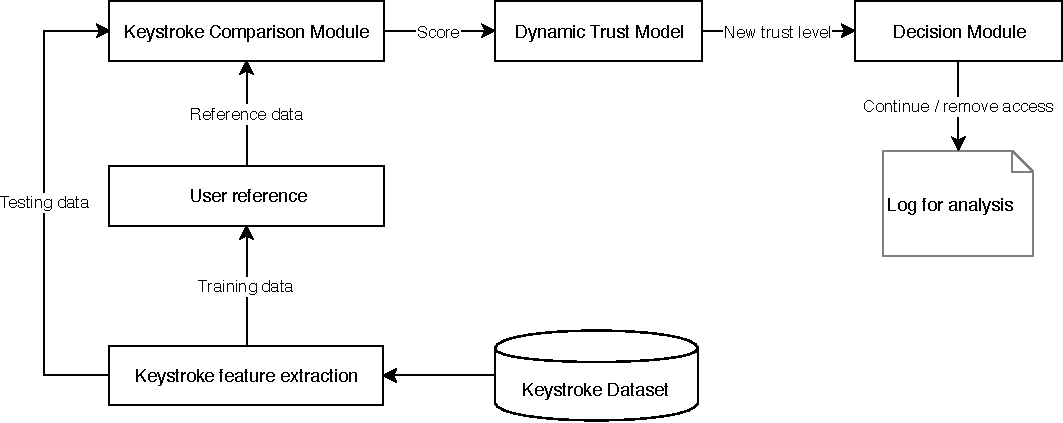
\includegraphics[width=0.9\textwidth]{figures/CA-diagram.pdf}
    \caption{Generalized diagram of the CA system's structure.}
    \label{fig:CA-diagram}
\end{figure}


\subsection{Feature extraction and references}
\label{sec:system-design-CA-ref}
Six features are utilized in the CA system, namely keycodes, monograph durations as well as PP, PR, RP and RR latencies from digraphs.
While certain systems in literature exclude monographs in their analysis, we found it necessary to consider them in our system.
If monographs were ignored, an attacker could wait for 1500 ms between keystrokes in order to avoid typing digraphs.
This would result in the system having little to no features available for matching, even if the user typed a full block of monographs.
Including monographs features helps mitigate this security issue.

\begin{table}[h]
\centering
\begin{tabular}{|l|l|}
\hline
Monograph & Digraph\\ \hline
- Keycode & - Keycode\\
- $\text{Duration}_{\text{Mean}, \sigma} $& - $\text{PP}_{\text{Mean}, \sigma}$\\
& - $\text{PR}_{\text{Mean}, \sigma}$  \\
& - $\text{RP}_{\text{Mean}, \sigma}$ \\
& - $\text{RR}_{\text{Mean}, \sigma}$
\\ \hline
\end{tabular}

\caption{The structure of the references used in our system. $\sigma$ is the standard deviation of recorded durations/latencies.}
\label{tab:reference-structure}
\end{table}
\Cref{tab:reference-structure} shows how these features are used in the reference.
For every feature occurring during enrollment, the system only stores the \textit{mean} and \textit{standard deviation} of the feature's recorded timing values.
All features are extracted as described in \Cref{sec:system-design-dataset}.
%Keycodes can also be considered a feature, but since all comparisons rely on identical keycodes, we will consider the durations and latencies.


As human behavior is prone to inconsistencies, removing outlier values can give more accurate representations of how a user typically behaves.
In PA systems, it is possible to remove outlier timing values from probe blocks, as each n-graph can have multiple recorded occurrences.
This is generally not the case for CA systems, as the trust level must be adjusted after every recorded keystroke.
However, it is possible to remove outliers from the CA reference.
We chose to so since our classifier relies on standard deviation, which causes it to be negatively affected by outliers.
For every feature in the reference, we removed outliers using Interquartile Range.
This was done within the scope of one feature. 
In other words, if a key were pressed only once and its duration were an outlier compared to other keys in the reference, it would still not be removed.
However, if the key had several occurrences, and therefore several durations, outlier durations would be removed if present.


\subsection{Matching}
\label{sec:system-design-CA-matching}
When processing a keystroke, its extracted features are handled by the Keystroke Matching Module which compares them to the genuine user's reference using a distance measure.
The comparison is performed by computing the dissimilarity score $sc$ between the probe timing features $p$ and the mean duration $\mu$ of the corresponding features from the same keycode in the reference.
This is calculated using the following formula:
$$ sc=\frac{1}{n}\sum_{i=1}^{n}\frac{|p_i-\mu_i|}{\sigma_i} $$
where $i$ is a specific feature, $n$ is the amount of available \textit{timing features} and $\sigma$ is the \textit{standard deviation} of the reference features.
Our implementation makes a distinction between monographs and digraphs in the sense that they produce two separate scores.
In practice, this causes $n$ to either be 1 (monograph duration) or 4 (digraph latencies).
For digraphs, this means that the score is the mean of the distances computed for the PP, PR, RP and RR latencies.

The formula is a variant of the Scaled Manhattan Distance, as described by Killourhy and Maxion \cite{Killourhy}.
They compared the performance of 14 different classifiers on static text keystroke dynamics, where Scaled Manhattan Distance achieved the best Equal Error Rate.
%Their variant uses mean absolute deviation for scaling the scores, while we have chosen standard deviation, 
This distance metric shows the dissimilarity between the probe and reference, and is used directly as the score input to the trust model.


\subsection{Trust model and decision module}
The trust model used in our system is a variant of the one presented by Mondal \cite{mondal}.
We have made certain changes to make it fit our system, and eliminated one parameter which was not used in our analysis.
\Cref{alg:trust-model} shows our implementation of the trust model.
Perhaps the most notable change is the fact that the function is inverted horizontally, as seen in \Cref{fig:sigmoids}.
This was a necessary feature due to having a dissimilarity score as input.

\begin{algorithm}[htbp]
 \KwData{\\
 $sc_i\gets$ Dissimilarity score for $i^{th}$ action\\
 $A\gets$ Threshold for reward or penalty\\
 $B\gets$ Width of sigmoid function\\
 $C\gets$ Maximum reward and penalty\\
 $Trust_{i-1}\gets$ Trust level after $(i-1)^{th}$ action\\
 }
 \KwResult{\\$Trust_i\to$ Trust level after $i^{th}$ action}
 \Begin{
 \begin{equation}
 \Delta_T(sc_i) = \text{min}\{-C + (\frac{C*2}{1 + \text{exp}(\frac{sc_i-A}{B})}), C\}
 \label{eq:delta-trust}
 \end{equation}
 \begin{equation}
 Trust_i = \text{min}\{\text{max}\{Trust_{i-1} + \Delta_T(sc_i), 0\}, 100\}
 \end{equation}
 }
 \caption{Algorithm for Trust Model}
\label{alg:trust-model}
\end{algorithm}

\begin{figure}[!htbp]
  \begin{subfigure}[b]{0.5\textwidth}
    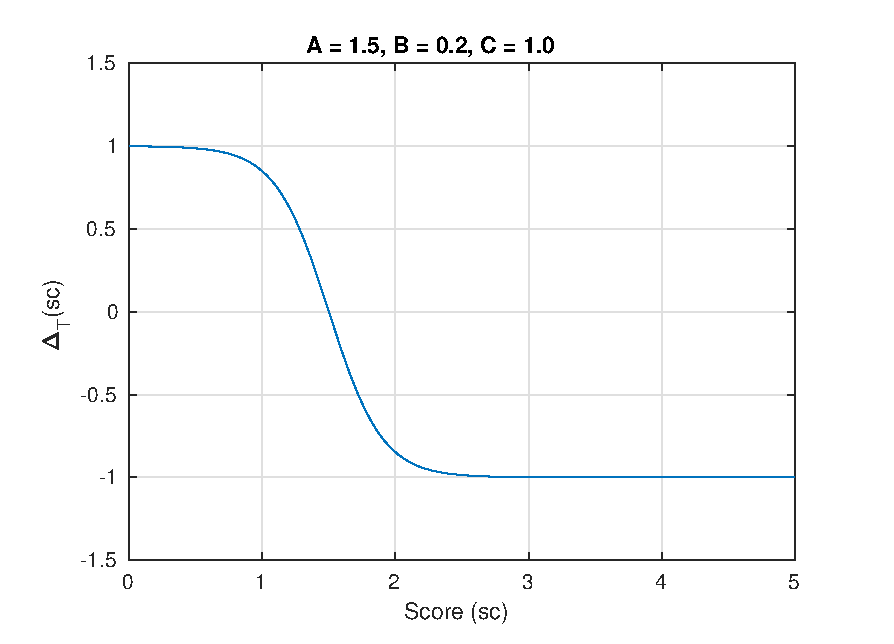
\includegraphics[width=\textwidth, height= 0.3\textheight]{figures/sigmoid1.eps}
    \label{fig:sigmoid1}
  \end{subfigure}
  \hfill
  \begin{subfigure}[b]{0.5\textwidth}
    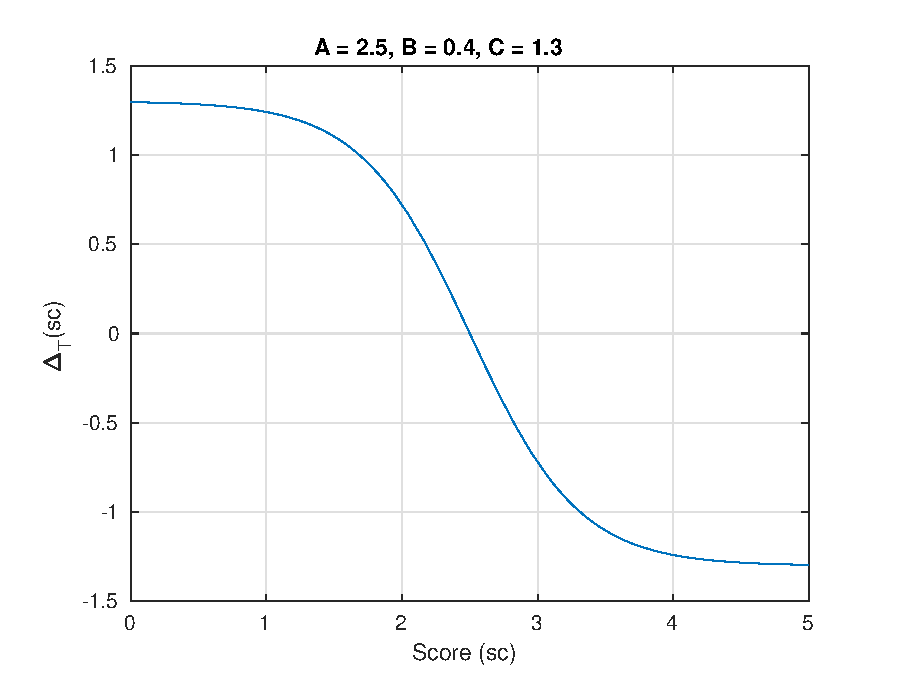
\includegraphics[width=\textwidth, height=0.3\textheight]{figures/sigmoid3.eps}
    \label{fig:sigmoid2}
  \end{subfigure}
  \caption{Examples of how the score would affect the trust level using different parameters for \Cref{eq:delta-trust}.}
  \label{fig:sigmoids}
\end{figure}

As mentioned in \Cref{sec:system-design-CA-matching}, monograph scores and digraph scores are separated.
In practice, this means that the $2^{\text{nd}}$ monograph of a valid digraph produces \textit{two} scores.
One score represents the monograph, while the other represents the digraph.
Therefore, a digraph produces \textit{three} scores in total: 2 monograph scores + 1 digraph score. 
This brought in the question of how to handle digraph actions at the lockout threshold.
For example, let the current trust level $Trust_{i-1} = 90.3$ and lockout threshold $T_{\text{lockout}} = 90$.
It is then possible that the next monograph score causes $Trust_i = 89.6$.
However, if the system locks the user out at that point, it disregards the fact that the monograph may be the $2^{\text{nd}}$ component of a digraph.
This issue is highlighted when the digraph score would have raised the trust level back to a value above $T_{\text{lockout}}$, for example $Trust_i = 90.2$.
Therefore, when observing digraph actions, the Decision Module locks the user out only if $Trust_i < T_{\text{lockout}}$ after considering both the monograph \textit{and} digraph scores of the keystroke.

\section{PA system}
The foundation of our PA system is based on that of Ferreira and Santos \cite{superResults}.
Some of their features, such as "progressive learning" has been excluded from our implementation.
When three consecutive probe blocks were accepted, their system would update the user's reference, infusing said probes into it in order to keep the reference up to date with the genuine user's most recent behavior.
The reason for not including this feature is threefold:
\begin{itemize}
    \item The dataset we used for analysis was collected over the course of about one week per user. The user's typical behavior is not expected to be significantly changed that quickly, eliminating the need for an adaptive reference.
    \item Even if this would slightly improve performance, our goal is not to necessarily create high performing CA or PA systems. 
    Instead, it is to observe the effect of combining them regardless of what their individual performances are.
    \item Updating the user's reference several times when testing system performance would severely impact processing time for full test runs. 
    This would in turn impact the amount of different parameter sets we would be able to test in the project's analysis phase.
    Therefore, we chose to prioritize testing as many sets of parameters as possible over including this feature.
    In a real-time system, the extra computational overhead would be trivial due to larger time periods between each update.
\end{itemize}
The following subsections further describe our implementation of the PA system.

\subsections{Feature extraction and references}
We have used the same reference for our PA system as described in \Cref{sec:system-design-CA-ref}, however, a different set of features is considered.
Ferreira and Santos \cite{superResults} consider monograph durations, digraph PP and RP, trigraph PP and 4-graph PP latencies.
In order to lessen computational effort, as well as 

\section{Combined system}


%\subsection{Outliers}
%----
%In PA systems, it is possible to remove outlier timing values from probes, as each n-graph can have multiple recorded durations or latencies.
%This is generally not the case for CA systems, as a the trust level is adjusted after every recorded keystroke.
%However, it is possible to remove outliers from the CA reference.
%When testing the CA system with the Scaled Manhattan Distance, its ANGA and ANIA values dropped significantly, down to 1116 and 173, respectively.
%While detecting imposters after only 173 keystrokes on average is a very good result seen in isolation, locking out the genuine users after 1116 keystrokes on average is far too often to be seen as a practically viable system.
%We were able to adjust parameters so that the ANGA was raised to approximately 4157, though the ANIA was also raised to 638.
%We were unable to separate or raise the values much further beyond this point.
%
%A plausible explanation for this is that Scaled Manhattan Distance already takes outliers into account by using standard deviations.
%When outliers were removed from the reference, the standard deviations for several n-graphs were drastically lowered, causing the classifier to be too strict. 
%In essence, it was demanding much less deviation from the mean than what can be realistically expected from the genuine user's natural behavior.
%Therefore, we decided to keep outliers in the reference for this version of the system.




%Our goal was to investigate the impact of combining periodic and continuous authentication.
%
%
%
%As our goal is not to achieve the best performing system, but rather to s % could be results
\chapter{Analysis}
\label{chap:analysis}
We have tested the performance of both individual systems as well as the combined system with several different parameters and settings.
This chapter describes these tests, their results and how they affected further analysis.
The results are discussed continuously throughout the sections.
During testing, we set up every user as a genuine user and ran all other users' test sets against the genuine user's reference, simulating \textit{zero-effort attacks}.
In zero-effort attacks, imposters are not actively trying to spoof or imitate the behavior of the genuine user, but rather type in their own speed and rhythm.
This describes a scenario where for instance the imposter is unaware of the CA/PA system running in the background of the genuine user's computer.

For every user in our dataset, there is one genuine user (them self) and 45 imposters.
As our dataset contains 46 genuine users, this gives us $46 \times 45 = 2070$ imposter runs every time we test the system's performance.
We have chosen to categorize and present certain test results similarly to Mondal's \cite{mondal} result presentations.
Using \Cref{tab:adjusting-SO-NO} as an example, users are then separated into the following four groups.
\begin{description}
    \item [+/+]: The genuine user was never locked out, and all imposters were locked out at some point, which is the best case scenario.
    \item [+/-]: The genuine user was never locked out, however at least one imposter was never locked out.
    \item [-/+]: The genuine user was locked out at least once, but so were all imposters.
    \item [-/-]: This is the worst case scenario. The genuine user was locked out at least once, and at least one imposter was never locked out.
\end{description}

We chose to do full test runs for every system configuration, meaning that all 46 users were included, and the full test sets of all imposters were used.
If the intention of this project was to propose biometric systems with certain performances using given sets of parameters, doing full test runs like this would lead to \textit{overfitting}.
However, our aim was to observe how different ways of combining CA and PA systems affected performance.
To observe this, full test runs were needed per configuration.
Replicating our systems with the exact same parameters is therefore likely to give different results, though one can expect to see similar \textit{effects} on base performances when adjusting parameters in the same way as we have done.

\Cref{sec:analysis-CA} describes how we tested the CA system and found the configuration to be used in the combined system. 
The testing of the PA system is described in \Cref{sec:analysis-PA}.
The results for the decision level fusion are discussed in \text{sec:analysis-decision-lvl}, while score level fusion results are presented in \Cref{sec:analysis-score-lvl}.
This chapter is concluded with a discussion on computational impact in \Cref{sec:analysis-computational-impact}.


\section{CA system}
\label{sec:analysis-CA}
The performance analysis of our stand-alone CA system is presented in this section.
This includes certain edge-case issues we had to account for, as well as the general performance using various parameters.

\subsection{Single and no occurrences}
\label{sec:analysis-CA-SONO}
Adjusting the fixed score for n-graph features having only a single occurrence (SO) in the reference had minimal impact on detection performance.
This was expected, as these are relatively rare.
For that reason, it is natural that features from probe actions either have none or several occurrences in the reference more often than only a single occurrence.
We observed that adjusting the fixed score for n-graphs missing in the reference had significant impact on the ANIA and ANGA ratings.

For example, when using the sigmoid function seen in \Cref{fig:sig185}, we tested adjusting the fixed score for single and no occurrences (NO).
The results of these tests can be found in \Cref{tab:adjusting-SO-NO}.
The CA system becomes more strict as the SO and NO scores are increased, as this means that the trust levels are affected more negatively.
However, it has a larger impact on ANIA than ANGA.
Furthermore, we also tested the impact of lowering the SO score while keeping the NO score near maximum.
The result of this test can be seen in the last section of \Cref{tab:adjusting-SO-NO}.
Compared to the section above, it seems that the NO score has a much larger impact.
We can also see that the performance was negatively affected by using a low SO score, as 4 more imposters went undetected, and one user was moved from the -/+ category to the -/- category.
Therefore, it seems that having harsh punishments for n-graphs not present or with only a single occurrence in the reference leads to better overall detection performance.
We continued testing the system using such harsh punishments.

\begin{figure}[h]
    \centering
    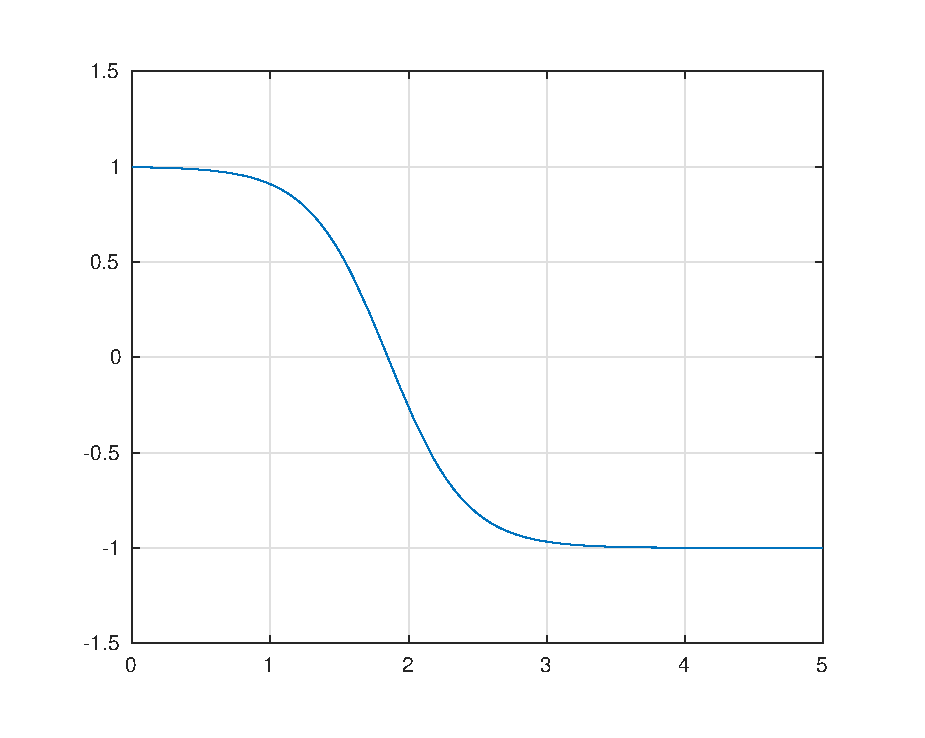
\includegraphics[width=0.5\textwidth]{figures/sig185.eps}
    \caption{Plot of the sigmoid function used to achieve the results in \Cref{tab:adjusting-SO-NO}.}
    \label{fig:sig185}
\end{figure}

\begin{table}[h]
\centering
\begin{tabular}{rlrrrr}
\hline
\textit{} & Category & \#Users & ANGA & ANIA & \#Imp. ND \\ \hline
\multirow{4}{*}{\textit{\begin{tabular}[c]{@{}r@{}}SO 2.0\\ NO 2.3\end{tabular}}} & +/+ & 6 & 139010 & 529 & 0 \\
 & +/- & 2 & 759945 & 4749 & 12 \\
 & -/+ & 24 & 4408 & 932 & 0 \\
 & -/- & 14 & 5110 & 3107 & 33 \\ \cline{2-6} 
 & Summary & 46 & 8973 & 1707 & 45 \\ \hline
\multirow{4}{*}{\textit{\begin{tabular}[c]{@{}r@{}}SO 2.3\\ NO 2.6\end{tabular}}} & +/+ & 5 & 13475 & 283 & 0 \\
 & +/- & 1 & 139525 & 5252 & 7 \\
 & -/+ & 35 & 3022 & 712 & 0 \\
 & -/- & 5 & 4071 & 2090 & 7 \\ \cline{2-6} 
 & Summary & 46 & 7240 & 914 & 14 \\ \hline
\multirow{4}{*}{\textit{\begin{tabular}[c]{@{}r@{}}SO 2.6\\ NO 2.9\end{tabular}}} & +/+ & 3 & 9372 & 251 & 0 \\
 & +/- & 1 & 139525 & 4335 & 5 \\
 & -/+ & 38 & 3041 & 596 & 0 \\
 & -/- & 4 & 3400 & 1499 & 6 \\ \cline{2-6} 
 & Summary & 46 & 6452 & 734 & 11 \\ \hline
\multirow{4}{*}{\textit{\begin{tabular}[c]{@{}r@{}}SO 3.0\\ NO 3.3\end{tabular}}} & +/+ & 3 & 9372 & 234 & 0 \\
 & +/- & 1 & 139525 & 4014 & 4 \\
 & -/+ & 38 & 2671 & 548 & 0 \\
 & -/- & 4 & 3396 & 1389 & 6 \\ \cline{2-6} 
 & Summary & 46 & 6146 & 676 & 10 \\ \hline
\multirow{4}{*}{\textit{\begin{tabular}[c]{@{}r@{}}SO 2.3\\ NO 3.3\end{tabular}}} & +/+ & 3 & 9372 & 249 & 0 \\
 & +/- & 1 & 139525 & 4747 & 7 \\
 & -/+ & 37 & 3064 & 556 & 0 \\
 & -/- & 5 & 3577 & 1646 & 7 \\ \cline{2-6} 
 & Summary & 46 & 6497 & 746 & 14 \\ \hline
\end{tabular}
\caption{CA results achieved by adjusting Single Occurrence (SO) and No Occurrences (NO) parameters. DTM parameters were $A = 1.85$, $B = 0.28$, $C = 1$ and $T_{\text{lockout}} = 90$.}
\label{tab:adjusting-SO-NO}
\end{table}

\subsection{Outlier removal}
\label{sec:analysis-CA-outliers}
In \Cref{sec:system-design-CA-ref}, we mentioned that we tested the CA system with and without outlier values in the reference.
When testing the system with these outliers removed, we observed a severe drop in both ANGA and ANIA ratings.
This essentially means that the system became more \textit{strict}, rapidly locking out both imposters and genuine users.
The reason for this lies in how our classifier (SMD) is scales Manhattan distances using standard deviation, which accounts for the dispersion of timing values.
The dispersion decreases when removing outliers, and a consequence is that the system expects keystroke features with less distance to the reference than before outlier removal.
Therefore, we had to make adjustments to the DTM's system level parameters to account for this change in expected user behavior.

The results in \Cref{tab:adjusting-SO-NO} were achieved \textit{without} outlier removal.
The parameters which gave an ANGA of 6146 and ANIA of 676 gave an ANGA of 1255 and ANIA of 218 when outliers were removed during reference construction.
We attempted to lower $T_{\text{lockout}}$ from 90 to 80 to make the system less strict, though this resulted in the ANIA rating increasing rapidly compared to the ANGA rating.
In other words, imposters gained too much of an advantage compared to the genuine user to justify this method for making the system more liberal.
%Lowering $T_{\text{lockout}}$ from 90 to 80 resulted in an ANGA of 4429 and ANIA of 787, which showed rapid growth of the ANIA rating compared to the ANGA rating's growth.

Lowering the DTM's "A" parameter to $1.3$ gave better results, which can be found in \Cref{tab:CA-outliers-removed-without-cutoff}.
These are comparable to the best result from \Cref{tab:adjusting-SO-NO}, being the 6146 ANGA and 676 ANIA.
Specifically the fourth row in \Cref{tab:CA-outliers-removed-without-cutoff} shows a result with 694 ANIA, only 18 actions more than the 676 ANIA without outlier removal.
Despite the small difference in ANIA ratings, the result \textit{with} outlier removal gave a significantly higher ANGA rating, as the genuine user could on average perform $8436-6146 = 2290$ more keypresses before being locked out.
With such positive results, we kept the outlier removal mechanism when combining the CA system with the PA system.
%The ANIA value of 676 \textit{without} outlier removal is comparable to the ANIA value of

\begin{table}[h]
\centering
\begin{subtable}[h]{0.45\textwidth}
\begin{tabular}{rrrr}
\hline
 $T_{\text{lockout}}$ & ANGA  & ANIA & \#Imp. ND  \\ \hline
 80                   & 1615  & 174  & 2          \\
 70                   & 3437  & 335  & 6          \\
 60                   & 5385  & 504  & 12         \\
 50                   & 8436  & 694  & 26         \\
 40                   & 10846 & 882  & 31         \\
 30                   & 12208 & 1103 & 50         \\
 20                   & 12981 & 1325 & 62         \\
 10                   & 13183 & 1503 & 69         
 \end{tabular}
 \caption{Without reference cutoff.}
 \label{tab:CA-outliers-removed-without-cutoff}
\end{subtable}
\hfill
\begin{subtable}[h]{0.45\textwidth}
\centering
\begin{tabular}{rrrr}
\hline
 $T_{\text{lockout}}$ & ANGA  & ANIA & \#Imp. ND \\ \hline
 80                   & 1569  & 159  & 2         \\
 70                   & 3283  & 299  & 5         \\
 60                   & 5297  & 450  & 10        \\
 50                   & 8362  & 625  & 21        \\
 40                   & 10622 & 798  & 25        \\
 30                   & 11871 & 1009 & 44        \\
 20                   & 12422 & 1180 & 52        \\
 10                   & 12727 & 1350 & 61       
\end{tabular}
\caption{With reference cutoff.}
\label{tab:CA-outliers-removed-with-cutoff}
\end{subtable}
\caption{CA results achieved with outlier removal using the following DTM parameters: $A= 1.3, B = 0.28 \text{ and } C=1$.}
\label{tab:CA-outliers-removed}
\end{table}

%\todo{Check all references to this chapter from System level chapter, and see if they need to be removed.}

\subsection{Reference cutoff}
\label{sec:analysis-cutoff}
When the individual CA and PA systems were implemented, a decision had to be made regarding the amount of keystroke data to be used in reference building.
As mentioned in \Cref{sec:system-design-dataset}, we use 35\% of the user's keystrokes recorded during data collection.
We tested the impact of limiting this amount to a maximum of 20000 keystrokes for users with exceptionally large datasets, so that the remaining training data could be used for testing instead.
Another motivating factor is that it leads to slightly less variance in reference quality between users.

The results in \Cref{tab:CA-outliers-removed} shows the impact of applying the reference cutoff.
We observed that both the ANGA and ANIA ratings as well as the number of undetected imposters generally were lowered as a consequence.
The difference was still minimal, and we concluded that it was reasonable to continue further analysis \textit{with} the reference cutoff.

\subsection{Personal and system level parameters}
\label{sec:CA-personal-parameters}
As our PA system has an element of \textit{personalization} in its lockout threshold, we faced the issue of personalizing the CA system as well before combining the systems.
The incentive to do so was that incorporating a personalized PA system into a CA system which only uses global parameters might be viewed as an unfair method for improving performance.
Therefore, we also built a version of our CA system which uses customized thresholds for rewards/penalties for each user.
\Cref{sec:CA-trust-and-decision} describes how the thresholds are calculated by using mean scores and tolerance levels.

Adjusting the tolerance level led to the results presented in \Cref{tab:CA-persRwrdThresh}, where using a tolerance level of 0.5 led to the most reasonable performance.
It was achieved with $T_{\text{lockout}}=50$, and can be compared to the result in \Cref{tab:CA-outliers-removed-with-cutoff} where also $T_{\text{lockout}} = 50$.
Whereas the ANIA dropped by an insignificant amount, the ANGA dropped from 8362 to 8087.
Though this was a negative change, the number of undetected imposters also dropped from 21 to 18, which slightly weighs up for the loss of ANGA rating.
Overall, these settings gave a satisfying performance and were used as the base when incorporating the PA system.

\begin{table}[h]
\centering
\begin{tabular}{rrrr}
\hline
Tolerance & ANGA  & ANIA & \#Imp. ND  \\ \hline
0   & 268   & 69  & 0  \\
0.1 & 770   & 93  & 0  \\
0.2 & 2107  & 143 & 3  \\
0.3 & 3951  & 218 & 3  \\
0.4 & 5671  & 381 & 5  \\
0.5 & 8087  & 623 & 18 \\
0.6 & 10461 & 986 & 36
\end{tabular}
\caption{CA results achieved with personal thresholds for reward/penalty. DTM parameters: \\$A=\text{ personal}, B = 0.28, C=1\text{, and } T_{\text{lockout}} = 50$.}
\label{tab:CA-persRwrdThresh}
\end{table}

\section{PA system}
\label{sec:analysis-PA}
\subsection{Reference cutoff}
The PA system's performance was tested with and without the reference cutoff, similarly to the CA tests discussed in \Cref{sec:analysis-cutoff}.
\Cref{tab:PA-cutoff} shows the cutoff's impact on performance. 
As in the case of the CA system, the impact is negligible.
Adjusting the tolerance level allowed us to balance the relation between FNMR and FMR, as mentioned in \Cref{sec:system-design-PA-decision}.
In other words, this parameter decided the system's strictness.
%The goal was to find a reasonable balance which had a high chance of detecting imposters 
%thereby controlling the tradeoff of catching imposters more quickly and locking out the genuine user more often.

When combining the CA and PA systems, the same sets of keystrokes had to be used to build the references and test sets.
This was needed due to the combined system using the exact same keystroke data for both the CA and PA subsystems during testing.
If the reference cutoff was used in only one of the subsystems, the test sets would contain different keystrokes, as the cutoff causes data from the reference portion of the dataset to be moved into the test portion.
The advantages given by the cutoff described in \Cref{sec:analysis-cutoff} also hold for the PA system.
Seeing as the impact of the cutoff was small for both systems, the cutoff was used in further analysis. This included testing of the combined system.

\begin{table}[h]
\centering
\begin{subtable}[h]{0.45\textwidth}
\begin{tabular}{rrrl}
\hline
Toler. & FNMR & FMR & \#Imp. ND  \\ \hline
0.02 & 47.51 & 4.68  & 2   \\
0.06 & 37.75 & 5.93  & 4   \\
0.10  & 30.25 & 7.47  & 4   \\
0.14 & 22.97 & 9.23  & 7   \\
0.18 & 17.77 & 11.48 & 9   \\
0.22 & 13.40 & 14.07 & 13  \\
0.26 & 9.44  & 17.11 & 17  \\
0.30 & 6.91  & 20.52 & 22  \\
0.35 & 4.70  & 25.37 & 37  \\
0.40 & 2.85  & 30.80 & 54  \\
0.45 & 1.80  & 36.67 & 87  \\
0.50 & 1.29  & 42.61 & 121
 \end{tabular}
 \caption{Without reference cutoff.}
 \label{tab:PA-without-cutoff}
\end{subtable}
\hfill
\begin{subtable}[h]{0.45\textwidth}
\centering
\begin{tabular}{rrrl}
\hline
Toler. & FNMR  & FMR & \#Imp. ND \\ \hline
0.02 & 48.08 & 4.68  & 2   \\
0.06 & 38.54 & 5.94  & 4   \\
0.10 & 30.04 & 7.50  & 4   \\
0.14 & 22.59 & 9.37  & 7   \\
0.18 & 17.36 & 11.70 & 9   \\
0.22 & 12.89 & 14.28 & 12  \\
0.26 & 9.29  & 17.42 & 18  \\
0.30 & 6.44  & 20.91 & 21  \\
0.35 & 3.85  & 25.88 & 36  \\
0.40 & 2.26  & 31.47 & 53  \\
0.45 & 1.51  & 37.45 & 88  \\
0.50 & 1.13  & 43.55 & 126
\end{tabular}
\caption{With reference cutoff.}
\label{tab:PA-with-cutoff}
\end{subtable}
\caption{Excerpt of PA results showing the performance impact of using a reference cutoff. A block size of 500 keystrokes was used.}
\label{tab:PA-cutoff}
\end{table}

\subsection{R- and A-distance weights}
Pinto et al. \cite{Pinto2014} studied how adjusting the weights of the R-and A-distances when combining them affected detection performance.
They found that 20\%-80\% weights for R- and A-distances was the best configuration for increasing the gap between average genuine and imposter scores while still considering the R-measure.
We tested our PA system using the same configuration to see how it affected its performance.
The result is illustrated as Detection error tradeoff (DET) curves in \Cref{fig:RAweights}.
The curves show that summing the R-and A-distances with equal weights outperforms the 80-20 weighting scheme for our PA system, as all FNMRs give lower tradeoffs for FMR with the equal weights scheme.

While we did not analyze the underlying reasons, it is worth pointing out that Pinto et al. used five different timing features where our system only uses three.
We also used a smaller block size of 500 keystrokes compared to their 750 keystrokes, and as mentioned in \Cref{sec:system-design-PA-comparison}, their dataset was limited.
All of these factors could play a role in why we had less success with their weighting scheme.
Equal weights were chosen for further analysis due to the superior performance.

\begin{figure}[ht]
    \centering
    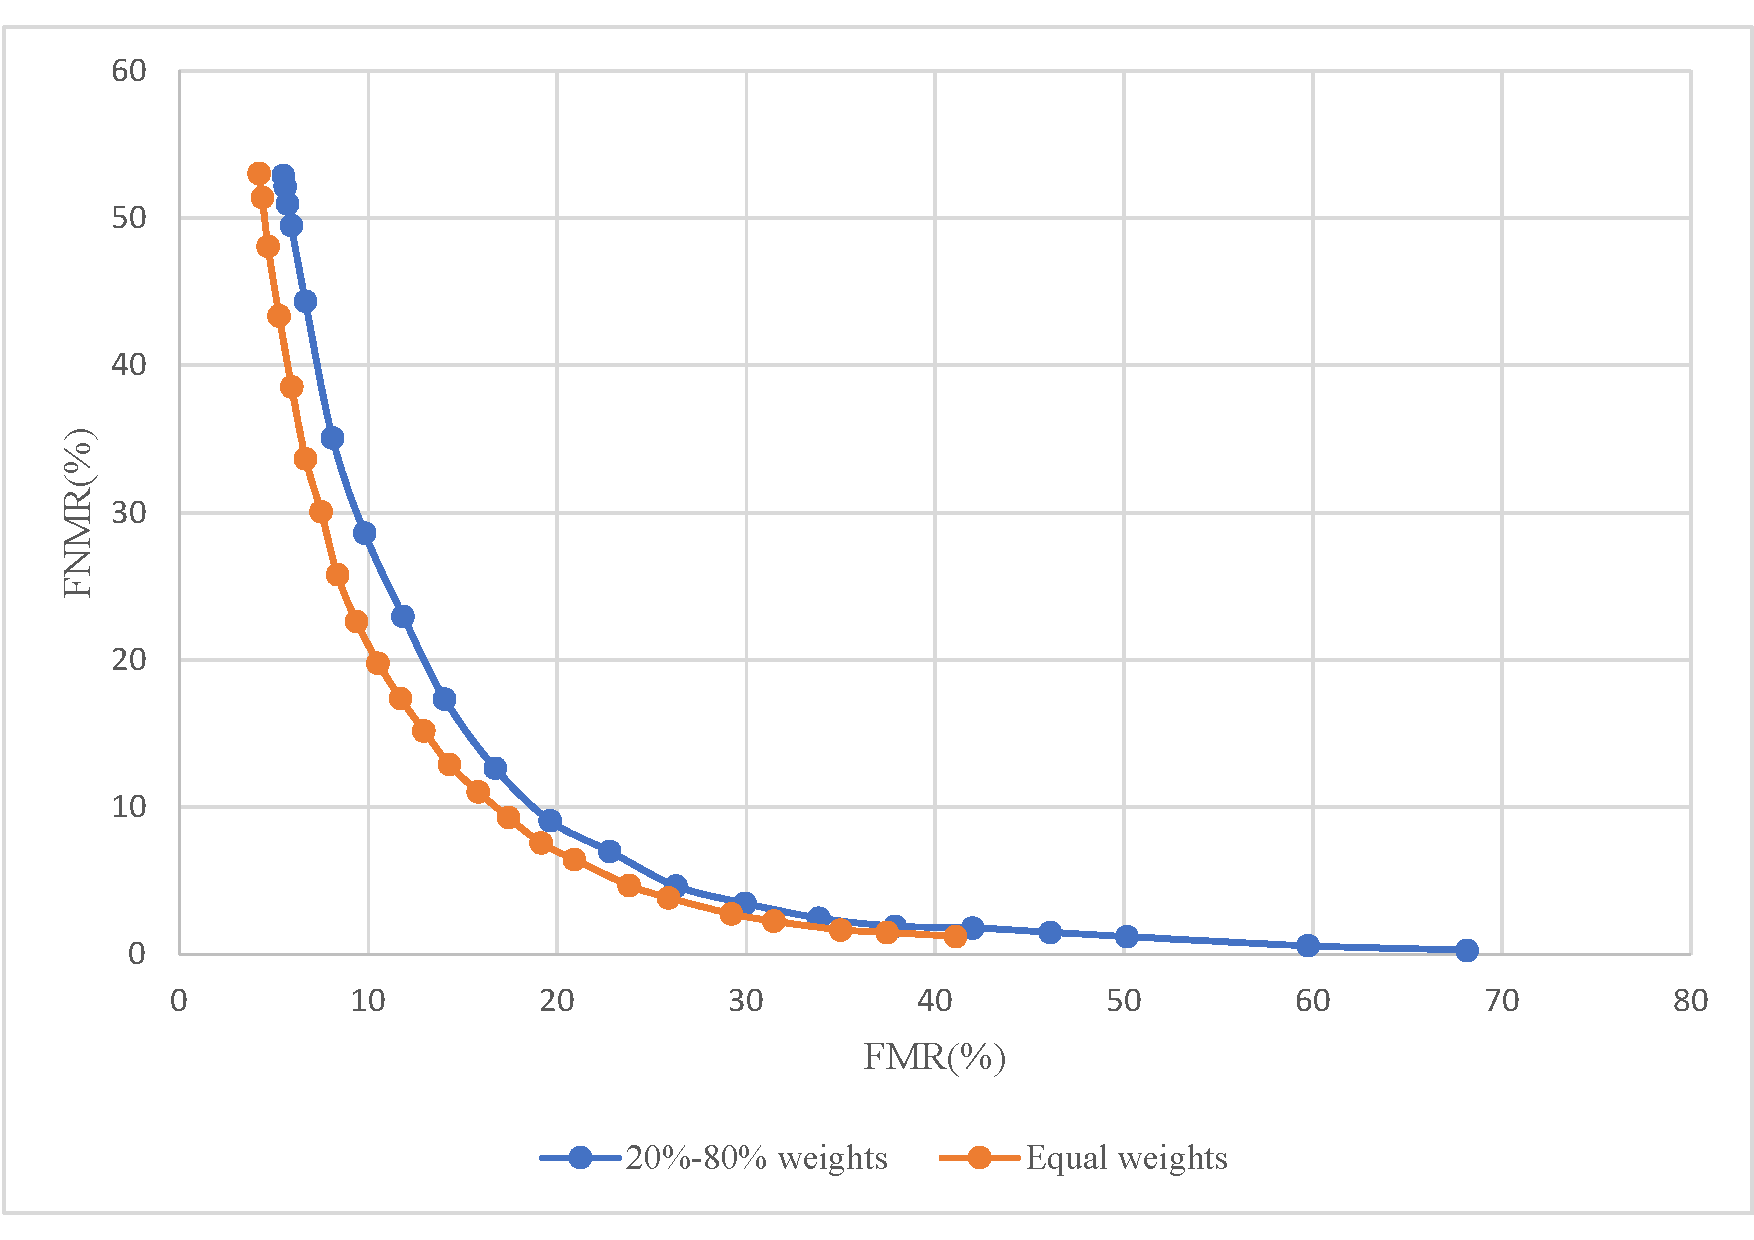
\includegraphics[width=1\textwidth]{figures/RAweights.pdf}
    \caption{Detection error tradeoff curves showing the detection performance of weighing R- and A-distances by 20-80\% respectively as well as using equal weights. }
    \label{fig:RAweights}
\end{figure}


\subsection{Block size}
\label{sec:analysis-PA-block-size}
Different block sizes were tested for the PA system.
These were 500, 250 and 100 keystrokes.
As a dissimilarity score is produced per block, the system has more information to base every dissimilarity score on when the block size is large.
This generally leads to more accurate decisions per block, and is reflected in the DET curves in \Cref{fig:block-lengths-ROC}.
There is a clear difference in detection accuracy between the block lengths that were tested, with 500 outperforming both of the other block sizes, and size 100 achieving the worst performance in terms of detection accuracy.

This does not necessarily imply that using a block size of 500 gives a \textit{better} PA system.
When the PA system waits for 500 keystrokes to be collected before processing probes, the imposter has a large window of access to the computer before they are locked out.
An example of an unfortunate scenario could be an imposter taking control over an unattended computer after the genuine user had either logged in or been successfully authenticated by the PA system without pressing any keys thereafter.
In both of these cases, the imposter would have free reign over the computer until they had typed 500 keystrokes, or until the genuine user returned to the workstation.

At first glance, this may seem like the worst-case scenario.
However, the imposter could also take control over the computer in the middle of a block, for example after 300 genuine keystrokes.
Ideally, they would be detected and locked out when the block was filled up, i.e. after only $500-300 = 200$ imposter keystrokes.
However, their window of opportunity could also become larger than 500.
The reason for this is that the genuine keystrokes making up the first 300 keystrokes of the block may outweigh the 200 imposter keystrokes, causing the probe to be accepted as \textit{genuine}, i.e. a match.
The PA system would then continue collecting keystrokes for the next block without locking the imposter out.
Their effective window of opportunity would then be $200+500 = 700$, giving them increased time to perform potentially harmful actions.

Situations like these highlight fundamental issues with PA systems and why such large block sizes can be problematic.
There is a tradeoff between higher detection performance and lower block sizes, which is why we tested the system with several block sizes.
All of these block sizes could then be used for testing the combined system later on.

\begin{table}[h]
\centering
\begin{subtable}[h]{0.45\textwidth}
\begin{tabular}{rrrr}
\hline
Toler. & ANGA  & ANIA & \#Imp. ND  \\ \hline
0.35 & 12989 & 675 & 36 \\
0.33 & 10670 & 656 & 31 \\
0.3  & 7760  & 632 & 21 \\
0.26 & 5383  & 605 & 18 \\
0.22 & 3880  & 583 & 12 \\
0.18 & 2880  & 566 & 9  \\
0.14 & 2213  & 552 & 7  \\
0.1  & 1664  & 541 & 4  \\
0.06 & 1298  & 532 & 4
 \end{tabular}
 \caption{Block size 500.}
 \label{tab:PA-block-size-500}
\end{subtable}
\hfill
\begin{subtable}[h]{0.45\textwidth}
\centering
\begin{tabular}{rrrr}
\hline
Toler. & ANGA  & ANIA & \#Imp. ND \\ \hline
0.5  & 12634 & 476 & 52 \\
0.45 & 8957  & 426 & 31 \\
0.43 & 7845	 & 409 & 27 \\
0.4  & 6124  & 386 & 19 \\
0.35 & 4302  & 354 & 16 \\
0.3  & 2920  & 329 & 11 \\
0.26 & 2198  & 313 & 8  \\
0.22 & 1665  & 300 & 6  \\
0.18 & 1252  & 290 & 2  
\end{tabular}
\caption{Block size 250.}
\label{tab:PA-block-size-250}
\end{subtable}

\begin{subtable}[h]{0.45\textwidth}
\centering
\begin{tabular}{rrrr}
\hline
Toler. & ANGA  & ANIA & \#Imp. ND \\ \hline
0.7  & 8288 & 395 & 98 \\
0.65 & 6531 & 335 & 66 \\
0.6  & 5028 & 286 & 38 \\
0.55 & 3779 & 247 & 30 \\
0.45 & 2112 & 192 & 12 \\
0.35 & 1136 & 157 & 3  \\
0.26 & 672  & 137 & 1  \\
0.18 & 433  & 125 & 0  \\
0.1  & 289  & 117 & 0  
\end{tabular}
\caption{Block size 100.}
\label{tab:PA-block-size-100}
\end{subtable}

\caption{PA results achieved with different block sizes and tolerance levels.}
\label{tab:PA-block-sizes}
\end{table}

The ANGA and ANIA rates of the PA system are calculated based on their FNMR and FMR rates and are presented in \Cref{tab:PA-block-sizes}, where the performance of the block sizes can be further compared.
An immediate observation is that small blocks sizes give lower ANIA rates than larger block sizes when similar ANGA rates are compared.
For example, when comparing results with approximately 2000 ANGA, the respective ANIA rates for block sizes 500, 250 and 100 are around 552, 313 and 192.
If were were to judge the performance solely based on ANGA and ANIA rates, it would seem that small block sizes are better.
However, the smaller block sizes tend to have significantly more undetected imposters.
Also, with higher ANGA rates, the smaller block sizes cause the system to often need more than one block to catch imposters.
While this is not necessarily a large issue in a stand-alone PA system with such small block sizes, problems can arise when combined with the CA system.
If the PA system can influence the trust level to be \textit{increased}, then the blocks that produce a false match before the imposter is detected will boost the trust level.
This can negate the CA system's own progress in detecting the imposter.
For instance, if the imposter's current trust level is 60, and $T_{\text{lockout}}=50$, a falsely matched block could increase the current trust level back to for example 90.
This would give the imposter a larger window of opportunity than if the PA system was not involved in the first place, as the CA system probably would have brought the trust level below $T_{\text{lockout}}$ a few moments later.
Smaller block sizes are therefore not necessarily the better option for the combined system.

\begin{figure}[h]
    \centering
    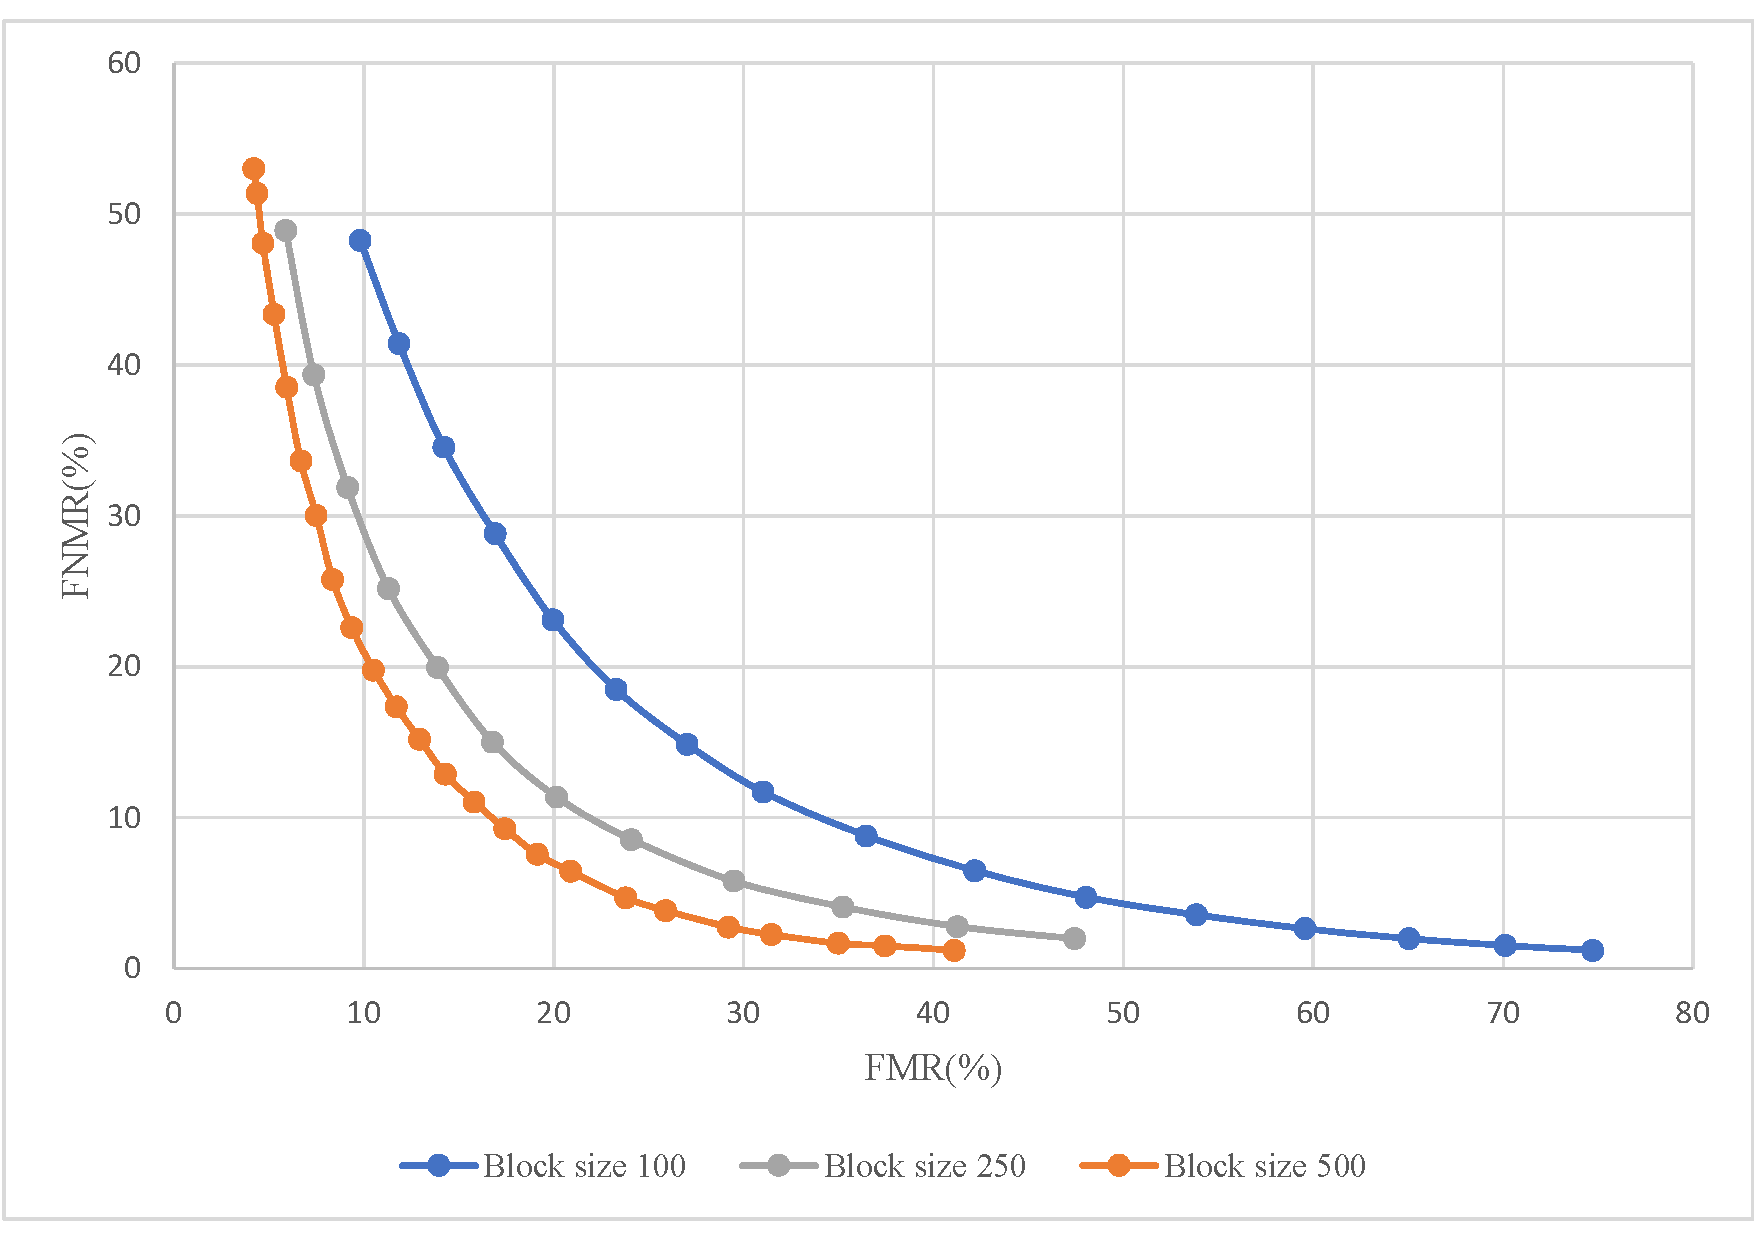
\includegraphics[width=1\textwidth]{figures/block-lengths-ROC.pdf}
    \caption{DET curves showing the performance for different block sizes.}
    \label{fig:block-lengths-ROC}
\end{figure}

\section{Decision level fusion}
\label{sec:analysis-decision-lvl}
This section presents results achieved by combining continuous and periodic authentication at the decision level.
The fusion scheme is based on the allowed range of trust $T_\text{range}$ as described in \Cref{sec:system-design-combined-score}.
As the CA configuration chosen for the combined system had $T_{\text{lockout}} = 50$, the allowed range of trust was $T_{\text{range}} = 100-50 = 50$.
When testing the decision level fusion, the binary decision of the PA subsystem would therefore increase or decrease the trust level by a specific amount between 0-50.
%Results from the decision level fusion are shown in \Cref{sec:analysis-decision-lvl}, while score level fusion results can be found in \Cref{sec:analysis-score-lvl}.
%The section is concluded with a discussion in \Cref{sec:analysis-discussion}.




%\subsection{}
%As described in \Cref{sec:system-design-combined-decision}, the decision level fusion scheme has the PA subsystem processing a probe block and sending a Match or Non-Match result to the CA system's DTM.
%The DTM then adjusts the current trust level according to the received result, by lowering or increasing it by specific amounts.

In order to control how much to increase or decrease the trust level, two parameters were used.
They were \textit{'UP'} and \textit{'DOWN'}, 
each representing how large a portion of $T_{\text{range}}$ to increase or decrease the current trust level by, respectively.
For instance, with $\textit{UP}=0.3$ and $\textit{DOWN}=0.6$, probe blocks producing a match would increase the trust level by $0.3 \times 50 = 15$.
Probes producing a non-match would decrease the trust level by $0.6 \times 50 = 30$.
Such a configuration would punish punish imposters more than it would reward the genuine user.

The \textit{UP} and \textit{DOWN} values were set as system level parameters, i.e. they were the same for all users per test.
Optimizing these values for each user using genetic algorithms or other optimization techniques is another option.
Such algorithms are however computationally expensive and time consuming, and were not used for this project.

Another example setting that we tested was $\textit{UP}=1$ and $\textit{DOWN}=0.6$.
\Cref{fig:decision-lvl-genuine-250BL} shows an except of testing this setting with User 1 as a genuine user, meaning that their test set was used against their own reference.
In the beginning, the user seemed to be typing in an unusual manner compared to their reference causing the CA subsystem to rapidly decrease the trust level.
After 108 keystrokes, the trust level went below $T_{\text{lockout}}$, marking the undesired event of locking out the genuine user.
The block size was 250 in this case, and since the CA subsystem locked out the user before the block was filled up, the PA subsystem did not get a chance to prevent the lockout.

The trust level was brought back up to 100 after the lockout, which simulated the user logging back in and continuing typing.
The PA subsystem started collecting keystroke data for a new block from that point onward.
After keystroke number 300, the trust level started sinking again, down to 75 at keystroke number 358.
At that point, a block of 250 keystrokes had been filled up since the lockout at keystroke number 108.
This triggered the PA system to process the block probe, which resulted in a match.
Here we can observe the advantage of combining the systems, as the PA match caused the trust level to be increased by $1 \times 50 = 50$, capped at the maximum value of 100.
Such positive adjustments have the potential to give the genuine more time before potentially being wrongfully locked out.
In this specific example, we can see that another block was filled up, processed and matched after the following 250 keystrokes, however the trust level was at that point already at 100.

\Cref{fig:decision-lvl-user2-vs-user1-BL250} shows a portion of a test run where an imposter was locked out four times over the course of around 1250 keystrokes.
At keystroke number 231, the trust level dipped to 50.2 before increasing slightly again, barely keeping the imposter logged in.
However, at keystroke number 250, the PA subsystem kicked in and reduced the trust level by $0.6 \times 50 = 30$, bringing it far below $T_{\text{lockout}}$.
As this meant that the imposter was locked out, the trust level was then brought back to 100, and the test run continued.

Keystroke number 500 shows another example of the cooperation between the two subsystems.
The PA subsystem brought the trust level down by 30, which was not quite enough to bring it below the threshold.
The CA subsystem was however able lock the user out a few keystrokes later due to the assistance it received just before.
Later on, the CA subsystem locked the imposter out at keystroke number 749, just one keystroke before the PA subsystem would have kicked in.
After that, the CA subsystem was unable to cause another lockout on its own.
However, at keystroke number 999, the PA subsystem brought the trust level down to 70, and later on brought it below the threshold at keystroke 1249.
Especially the last two PA influences show how using the statistical information available in block probes can be beneficial to utilize in a combined CA/PA system.

\begin{figure}[htbp]
\centering
\begin{subfigure}[b]{0.8\textwidth}
   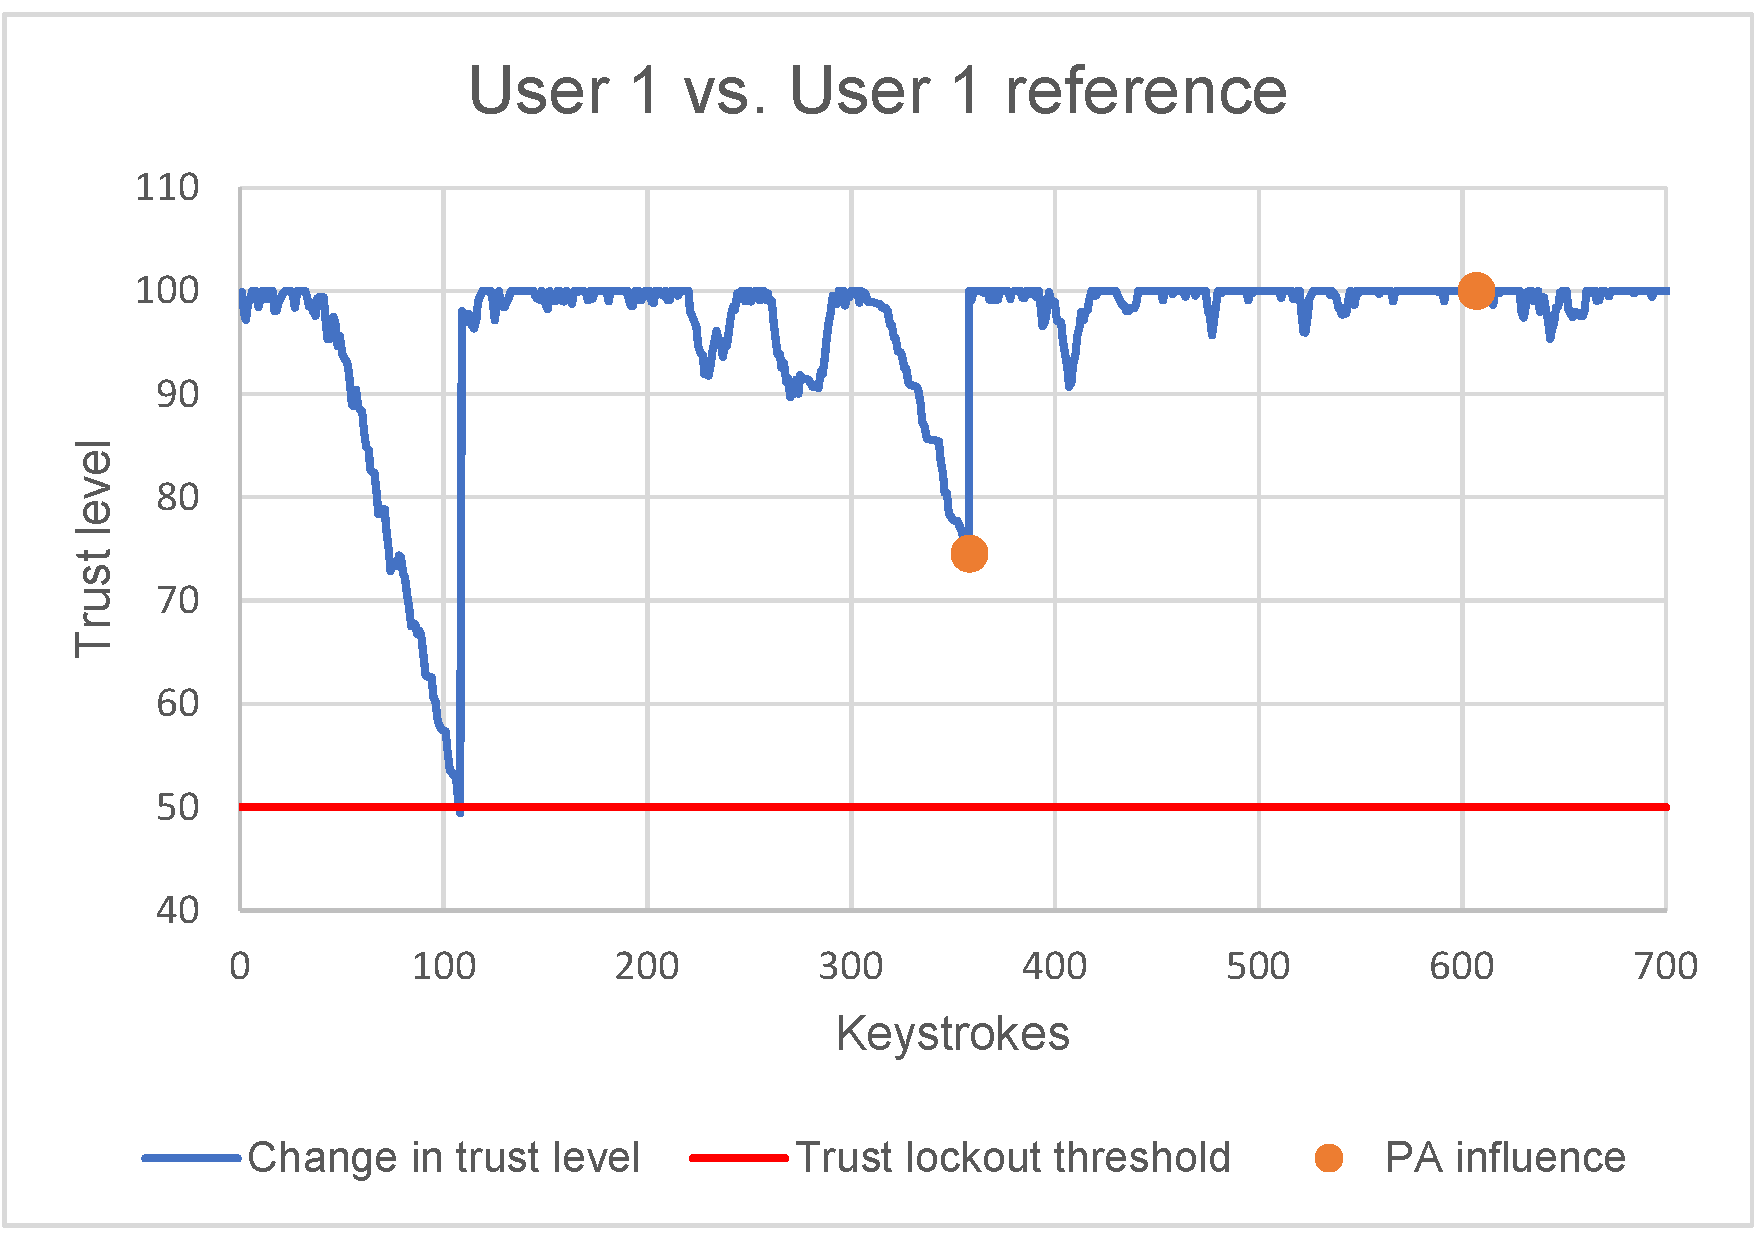
\includegraphics[width=1\linewidth]{figures/decision-lvl-genuine-250BL.pdf}
   \caption{User 1 as genuine user.}
   \label{fig:decision-lvl-genuine-250BL} 
\end{subfigure}

\begin{subfigure}[b]{0.8\textwidth}
   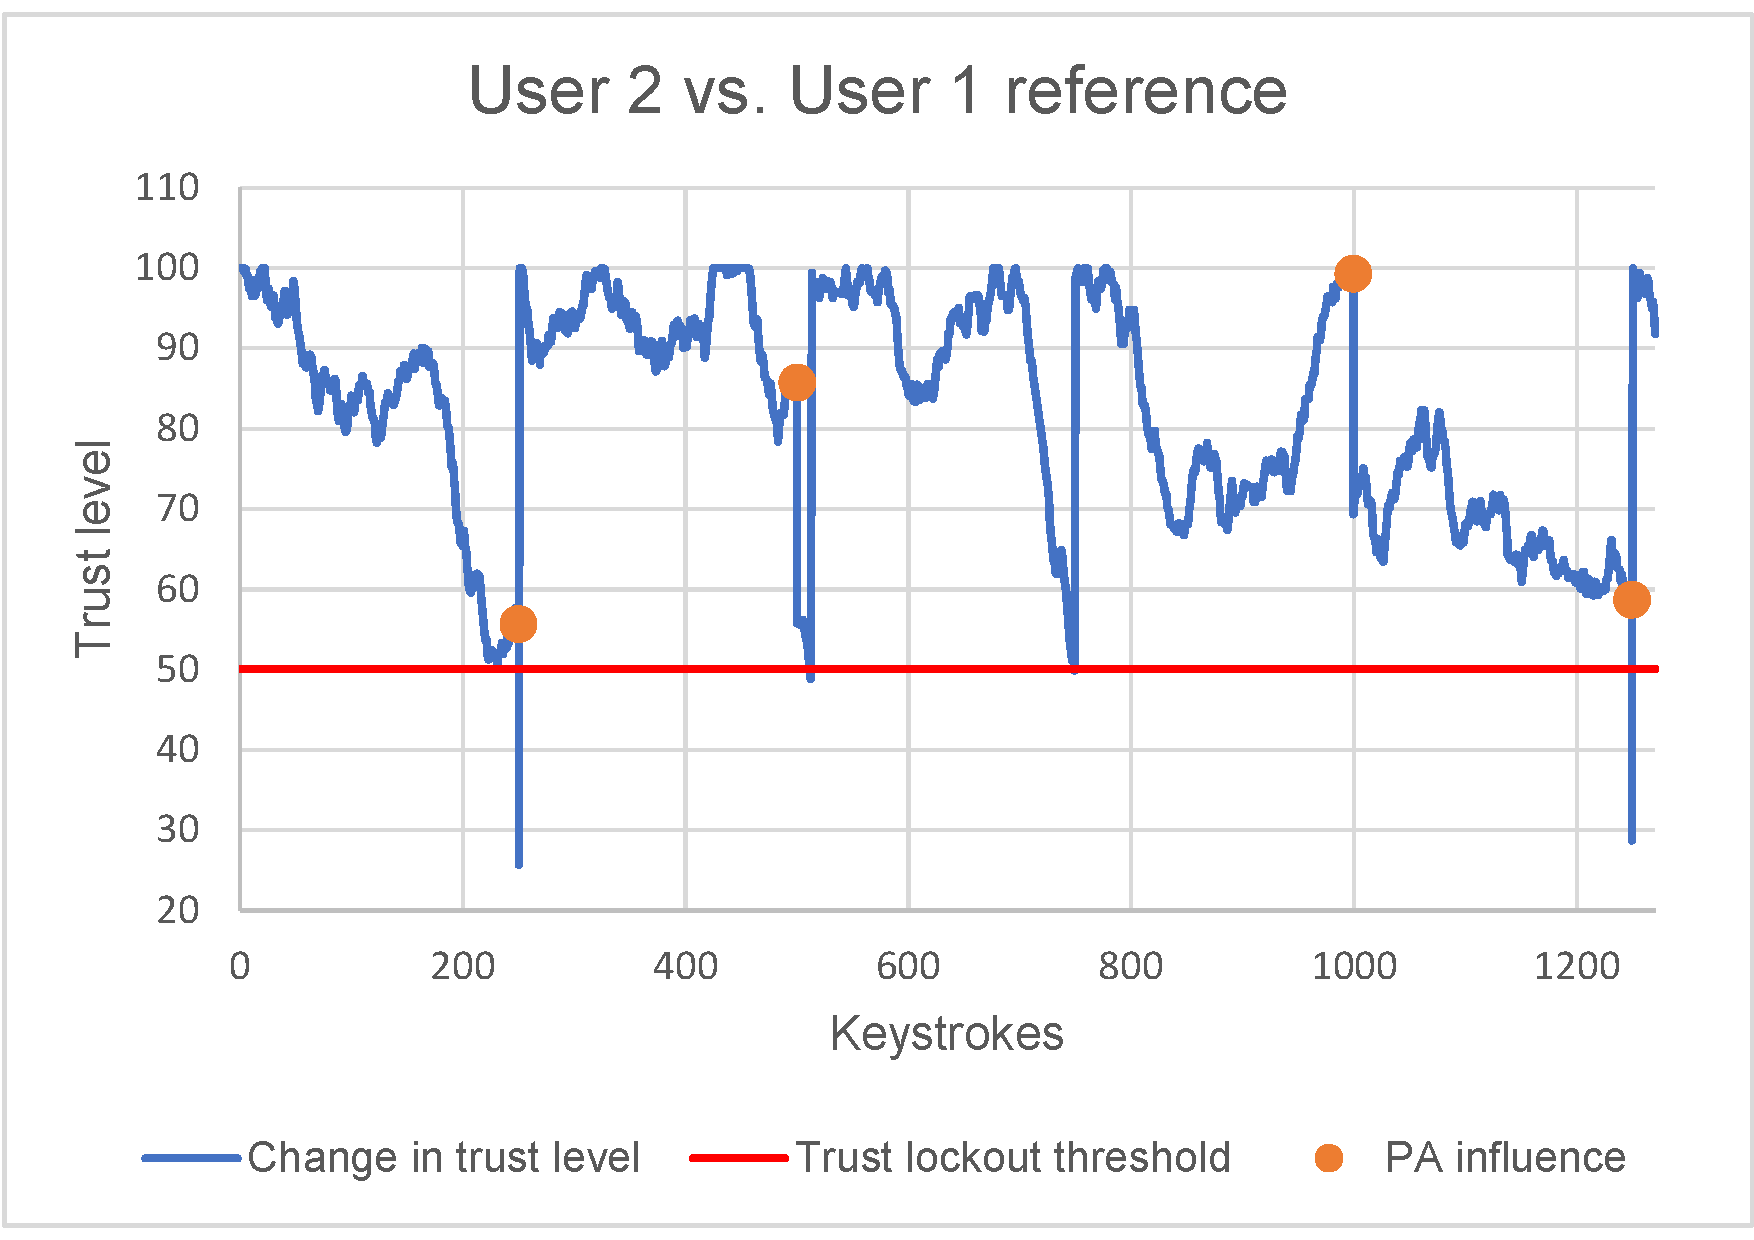
\includegraphics[width=1\linewidth]{figures/decision-lvl-user2-vs-user1-250BL.pdf}
   \caption{User 2 as imposter vs User 1's reference.}
   \label{fig:decision-lvl-user2-vs-user1-BL250}
\end{subfigure}

\caption{Examples of decision level fusion with $\text{block size} = 250$. $\textit{UP} = 1, \textit{DOWN} = 0.6$.}
\label{fig:decision-lvl-user1-example}
\end{figure}

\subsection{Results}

Before looking at how the incorporation of the PA system had on the original CA system's performance, we will discuss some observations regarding the impact of the decision level fusion's parameters.
The first observation to mention is that adjusting the \textit{DOWN} parameter generally had a larger impact on detection performance than the \textit{UP} parameter.
An example of this can be seen in \Cref{tab:UD-difference-1.001,tab:UD-difference-0.4}, as the performance difference between them was negligible even with a considerable difference in \textit{UP} values.
However, adjusting the \textit{DOWN} parameter from 0 to 1.001 caused a difference of almost 4000 ANGA and over 400 ANIA.
The reason for testing $\textit{DOWN}=\text{1.001}$ was the same as explained in \Cref{sec:system-design-combined-score}; it allowed the PA subsystem's influence to cause a direct lockout even when the current trust level was at its maximum.
As seen in the tables, the extra 0.001 in \textit{DOWN} value showed its effect by causing a drop in both ANGA and ANIA. 
However, the ANGA showed a drop of $6366-6018 = 348$ in \Cref{tab:UD-difference-1.001}, while the ANIA only dropped by $306-298 = 8$.
%In the same table we can see similar drops in ANGA where the corresponding ANIA drop is around 50.
%What this means is that the benefit of being able to lock out imposters who are currently at trust level 100 is small compared tcatching imposters 8 keystrokes earlier on average has a large negative consequence
This indicates that letting the PA subsystem lock out users who are currently at trust level 100 has large consequences for genuine users compared to the benefit of locking out imposters faster.
This makes sense, as a user at trust level 100 is more likely to be the genuine user than an imposter.
When these genuine users are wrongfully brought from trust level 100 to below $T_{\text{lockout}}$, the CA subsystem is given no chance to correct the PA subsystem's mistake.
Since imposters spend more time below trust level 100, reducing their trust level by $1\times T_{\text{range}}$ will often bring them far below $T_{\text{lockout}}$ which could be considered an "overkill".
Therefore, the extra 0.001 punishment is less likely to make a difference for them than for genuine users.
This ties into our \textit{research sub-question 3}, as it seems that having the PA subsystem adjust the trust level is generally better than guaranteeing that a non-match results in an instant lockout.
In spite of this, we continued testing $\textit{DOWN} = \text{1.001}$ to see if similar behavior was shown for other settings as well.

The reason for testing $\textit{UP} = \text{1.001}$ instead of 1 is simply that we originally tested the system using equal values for \textit{UP} and \textit{DOWN}, and $\textit{DOWN} = \text{1.001}$ was needed for the reason mentioned above.
The extra 0.001 for the \textit{UP} parameter makes no difference in practice, and was only used for convenience.
What does however make a difference for the \textit{UP} parameter is giving it a low value, usually below 0.4.
At such low values, the tests showed an exception to the general behavior being that adjustment of \textit{UP} makes little to no difference.
This can be seen in \Cref{tab:UD-difference-0.2}, where $\textit{UP} = \textit{0.2}$.
When comparing these results to the other two tables, we can see that it gave lower ANGA ratings for similar ANIA ratings.
In other words, using such a low \textit{UP} gave a worse performance across the board.

A likely explanation is that some genuine users have benefited largely by being ‘saved’ by the PA system at certain times, when their trust level was low.
With smaller \textit{UP} values, the PA subsystem had less power in preventing the CA subsystem from wrongfully locking them out, and so the small boost in trust level may not have been enough to keep them logged in for much longer.
Therefore, most of the following results presented in this section were achieved using a high \textit{UP} value.
%While we have tested various \textit{UP/DOWN} combinations, most of the results in this section will be summarized and presented with equal values for the two parameters due to the low impact of the UP value.
%In other words, they will represent the performance of equally rewarding genuine users and punishing imposters.
%We will also show certain exceptions, i.e. where adjusting the \textit{UP} parameter caused interesting and positive results. 


\begin{table}[ht]
\centering
\begin{subtable}[h]{0.45\textwidth}
\begin{tabular}{lrrr}
\hline
\textit{DOWN} & ANGA  & ANIA & \#Imp. ND \\ \hline
%0     & 8944 & 706 & 25(1.2\%) \\
%0.2   & 8602 & 630 & 20(1\%)   \\
%0.4   & 8025 & 569 & 16(0.8\%) \\
%0.6   & 7380 & 499 & 12(0.6\%) \\
%0.8   & 7062 & 432 & 12(0.6\%) \\
%1     & 5604 & 284 & 3(0.1\%)  \\
%1.001 & 5239 & 273 & 2(0.1\%) THIS IS BL250 WITH 1.001 UP.
0     & 8547 & 644 & 19(0.9\%) \\
0.2   & 8545 & 605 & 18(0.9\%) \\
0.4   & 8263 & 564 & 15(0.7\%) \\
0.6   & 8089 & 508 & 11(0.5\%) \\
0.8   & 7676 & 445 & 8(0.4\%)  \\
1     & 6278 & 307 & 3(0.1\%)  \\
1.001 & 6019 & 299 & 3(0.1\%)  
\end{tabular}
 \caption{\text{$\textit{UP}=1.001$}}
 \label{tab:UD-difference-1.001}
\end{subtable}
\hfill
\begin{subtable}[h]{0.45\textwidth}
\centering
\begin{tabular}{lrrr}
\hline
\textit{DOWN} & ANGA  & ANIA & \#Imp. ND  \\ \hline
%0     & 8936 & 690 & 25(1.2\%) \\
%0.2   & 8594 & 620 & 20(1\%)   \\
%0.4   & 8017 & 557 & 16(0.8\%) \\
%0.6   & 7352 & 493 & 12(0.6\%) \\
%0.8   & 7068 & 426 & 12(0.6\%) \\
%1     & 5607 & 282 & 3(0.1\%)  \\
%1.001 & 5223 & 270 & 2(0.1\%) THIS IS BL250 WITH 0.4 UP
0     & 8543 & 642 & 19(0.9\%) \\
0.2   & 8541 & 603 & 18(0.9\%) \\
0.4   & 8261 & 563 & 15(0.7\%) \\
0.6   & 8088 & 507 & 11(0.5\%) \\
0.8   & 7676 & 444 & 8(0.4\%)  \\
1     & 6366 & 306 & 3(0.1\%)  \\
1.001 & 6018 & 298 & 3(0.1\%)  
 \end{tabular}
\caption{$\textit{UP} = 0.4$}
\label{tab:UD-difference-0.4}
\end{subtable}
\begin{subtable}[h]{0.45\textwidth}
\centering
\begin{tabular}{lrrr}
\hline
\textit{DOWN} & ANGA  & ANIA & \#Imp. ND  \\ \hline
0     & 8134 & 638 & 19(0.9\%) \\
0.2   & 8132 & 599 & 18(0.9\%) \\
0.4   & 7850 & 558 & 15(0.7\%) \\
0.6   & 7676 & 503 & 11(0.5\%) \\
0.8   & 7264 & 441 & 8(0.4\%)  \\
1     & 5869 & 304 & 3(0.1\%)  \\
1.001 & 5612 & 296 & 3(0.1\%)  
 \end{tabular}
\caption{$\textit{UP} = 0.2$}
\label{tab:UD-difference-0.2}
\end{subtable}

\caption{Differences in performance when adjusting \textit{DOWN} parameter for different \textit{UP} values. Block size was 500 and PA tolerance was 0.33.}
\label{tab:UD-difference}
\end{table}

In this analysis, we will mainly focus on two types of performance improvement introduced by the combination, both regarding ANGA and ANIA ratings.
Recall that the specific settings used for the CA subsystem resulted in 8087 ANGA and 623 ANIA.
Our focus areas are then as follows:

\begin{description}
    \item [ANGA improvements:] For settings giving around 623 ANIA, we are interested in ANGA ratings above 8087.
    \item [ANIA improvements:] Where the ANGA ratings are around 8087, we are looking for ANIA ratings below 623.
\end{description}
Some other results of interest will also be discussed, such as how far up the combination was able to boost the ANGA beyond the original system while accepting the compromise of a higher ANIA.

\subsubsection{Block size 500}
After having described the general effects of the \textit{UP} and \textit{DOWN} parameters, we can discuss how the original CA system's performance was affected by incorporating the PA system, which was the main goal of the analysis phase.
The first block size tested was 500 keystrokes.
From the PA results in \Cref{tab:PA-block-size-500}, we chose to use a tolerance level of 0.33, as it gave an ANGA of 10670 and ANIA of 656.
Having such a high ANGA while still having an ANIA comparable to the CA system's ANIA of 623 seemed beneficial for the combined system, and was the reason for choosing this PA setting.
The underlying FNMR and FMR rates which were used for calculating the ANGA and ANIA were 4.69\% and 23.8\%, respectively.
The original CA system's performance is presented with more detail in \Cref{tab:CA-detailed-performance}.

Looking back at \Cref{tab:UD-difference-1.001}, we can see that the mentioned PA configuration was indeed able to positively affect the CA system's performance.
With $\textit{DOWN} = \text{0.2}$, the results were a higher ANGA for a slightly lower ANIA.
Specifically, the genuine users were able to type $8545-8087 = 458$ more keystrokes on average before being locked out, which is an increase of 5.66\%.
The ANIA was impacted more heavily, as seen where $\text{DOWN} = \text{0.6}$.
With an almost identical ANGA to that of the original CA system, the ANIA was lowered by $\text{623}-\text{508} = \text{115}$ which is an improvement of 18.46\%.
This means that imposters were caught significantly quicker on average with the combined system, confirming our main research question.
Also, the number of imposters that were never detected was reduced from 18 to 11.

Lastly, we can point out that for this block size, the ANGA saturated around 8545.
Increasing it any further beyond that point only resulted in a worse ANIA.
However, by sacrificing $\text{8087} - \text{6278} = \text{1809}$ ANGA, the ANIA dropped by 50.72\% down to 307, as seen where $\textit{DOWN} = \text{1}$.
With that setting, only 3 out of 2070 imposters were undetected.
%The general observed behavior of the decision level fusion is that increasing the \textit{U/D} values causes a decrease of both ANGA and ANIA.
%IS THIS DESCRIBED EARLIER?

\begin{table}[ht]
\centering
\begin{tabular}{lrrrr}
\hline
\textit{} Category & \#Users & ANGA & ANIA & \#Imp. ND \\ \hline
+/+ & 6  & 17409 & 269  & 0  \\
+/- & 1  & 12256 & 485  & 1  \\
-/+ & 30 & 6682  & 390  & 0  \\
-/- & 9  & 6091  & 1650 & 17 \\ \hline
Summary & 46 & 8087  & 623  & 18 \\ \hline
\end{tabular}
\caption{Detailed performance results of the CA configuration used in the combined system. \todo{Is this needed? Should it only be included later?}}
\label{tab:CA-detailed-performance}
\end{table}

%As \Cref{tab:UD-difference-BL500} shows an excerpt of the results achieved for the mentioned configuration, we refer to it for the discussion of this specific setting.
%Our first observation was that the ANGA rating peaked when \textit{UP and DOWN} (\textit{U/D}) was 0.3.
%The general observed behavior of the decision level fusion is that increasing the \textit{U/D} values causes a decrease of both ANGA and ANIA.
%However, these specific results show that only the ANIA increases when \textit{U/D} goes below 0.3, while the ANGA decreases.
%Strictly speaking, this is the opposite of what is wanted from a system like ours, as the optimal development would be an increasing ANGA coupled with a decreasing ANIA.
%A likely explanation is that one or more genuine users have benefited largely by being ‘saved’ by the PA system at certain times. 
%The less impact the \textit{UP} parameter is given, the less impact the boost of trust level has, and so the boost may not have been enough to keep them logged in.
%This is however a special behavior that was not seen in other block sizes, and is probably specific to our dataset.


%\begin{table}[ht]
%\centering
%\begin{tabular}{lrrr}
%\hline
%\textit{U/D} & ANGA  & ANIA & \#Imp. ND \\ \hline
%0.1   & 8087 & 608 & 17(0.8\%) \\
%0.2   & 8132 & 599 & 18(0.9\%) \\
%0.3   & 8332 & 580 & 15(0.7\%) \\
%0.4   & 8261 & 563 & 15(0.7\%) \\
%0.5   & 8130 & 542 & 14(0.7\%) \\
%0.6   & 8086 & 508 & 11(0.5\%) \\
%0.7   & 7819 & 475 & 8(0.4\%)  \\
%0.8   & 7676 & 445 & 8(0.4\%)  \\
%0.9   & 7361 & 388 & 5(0.2\%)  \\
%1     & 6278 & 307 & 3(0.1\%)  \\
%1.001 & 6019 & 299 & 3(0.1\%)  
%\end{tabular}
%\caption{Performance results for block size 500, with equal \textit{UP} (U) and \textit{DOWN} (D) values.}
%\label{tab:decision-level-BL500-equal}
%\end{table}

\subsubsection{Block size 250}
We were interested in seeing if smaller block sizes also could improve performance, as it would allow the PA system to engage more often, possibly detecting imposters more effectively.
\Cref{tab:decision-level-BL250} shows test results using 250 keystrokes as block size.
The PA tolerance used was 0.4, and as seen in \Cref{tab:PA-block-size-250}, it gave 6124 ANGA and 386 ANIA, calculated from an FNMR of 4.08\% and FMR of 35.24\%.
As mentioned in \Cref{sec:analysis-PA-block-size}, using a PA configuration with an ANIA rating too far from the block size could end up falsely matching imposter blocks too regularly, boosting their trust level and essentially preventing them from being detected by the CA system.
This was the reason for not choosing a more liberal setting for this block size.

\begin{table}[ht]
\centering
\begin{tabular}{lrrr}
\hline
\textit{DOWN} & ANGA  & ANIA & \#Imp. ND \\ \hline
0     & 8944 & 706 & 25(1.2\%) \\
0.1   & 8944 & 663 & 22(1.1\%) \\
0.2   & 8602 & 630 & 20(1\%)   \\
0.4   & 8025 & 569 & 16(0.8\%) \\
0.6   & 7380 & 499 & 12(0.6\%) \\
0.8   & 7062 & 432 & 12(0.6\%) \\
1     & 5604 & 284 & 3(0.1\%)  \\
1.001 & 5239 & 273 & 2(0.1\%) 
\end{tabular}
\caption{Performance results for $\text{block size} = \text{250}$, $\text{PA tolerance} = \text{0.4}$ and $\textit{UP} = \text{1.001}$.}
\label{tab:decision-level-BL250}
\end{table}

Block size 250 seems to be less successful in improving the CA system's ANIA rating compared to block size 500. 
In the fourth row of \Cref{tab:decision-level-BL250}, we see that even though the ANGA was lower than the 8089 ANGA in \Cref{tab:UD-difference-1.001}, it had a higher ANIA.
Still, an interesting observation is that the lower block size was able to boost the ANGA to 8602 with only $\text{630}-\text{623} = \text{7}$ higher ANIA than the original CA system, which is also slightly higher than what was achieved with block size 500.
Furthermore, it was able to bring the ANGA up to 8944 when accepting an ANIA increase of $\text{663}-\text{623}=\text{40}$.

\subsubsection{Block size 100}
For the smallest block size, we used a PA tolerance of 0.26.
This had quite low performance ratings, namely 672 ANGA and 137 ANIA, as seen in \Cref{tab:PA-block-size-100}.
Again, we saw this as necessary in in order to avoid boosting imposter trust levels too often.
The results can be found in \Cref{tab:decision-level-BL100}, where we see some similar effects as with block size 250.
For reducing ANIA without sacrificing ANGA, this block length was the worst performer of the three block sizes.
This is evident by looking at the result where $\textit{DOWN} = \text{25}$.
By comparing this result to block size 250 in \Cref{tab:decision-level-BL250} where $\text{DOWN} = \text{0.4}$, we see a lower ANGA together with a higher ANIA with block size 100.

\begin{table}[ht]
\centering
\begin{tabular}{lrrr}
\hline
\textit{DOWN} & ANGA  & ANIA & \#Imp. ND \\ \hline
0.1   & 8992 & 748 & 31(1.5\%) \\
0.2   & 8737 & 636 & 23(1.1\%) \\
0.25  & 7919 & 581 & 18(0.9\%) \\
0.4   & 6815 & 438 & 9(0.4\%)  \\
0.6   & 5135 & 301 & 5(0.2\%)  \\
0.8   & 3686 & 224 & 3(0.1\%)  \\
1     & 973  & 134 & 0(0\%)    \\
1.001 & 769  & 126 & 0(0\%)  
\end{tabular}
\caption{Performance results for $\text{block size} = \text{100}$, $\text{PA tolerance} = \text{0.26}$ and $\textit{UP} = \text{1.001}$.}
\label{tab:decision-level-BL100}
\end{table}

Similarly to block size 250, we also see an ability to boost ANGA for the compromise of higher ANIA.
We also see that it was able to bring both ANGA and ANIA ratings far down.
This is however likely due to the low PA tolerance of 0.26, which is a fairly strict setting causing probe blocks from both imposters and genuine users to be relatively likely to result in a non-match. 
Specifically, the underlying FNMR was 14.87\% and FMR was 27.02\%.
The result was therefore a highly sensitive \textit{DOWN} parameter, giving a large range between the most liberal and most strict setting.

\subsubsection{Other tolerance levels}
Lastly, it should be pointed out that different tolerance levels for each block size was tested to see what effect adjusting it up or down had.
In general, this resulted in worse performance, and the tolerance levels previously discussed produced the best results.
\todo{Refer to correct attachment when it's inserted.}

%
%\begin{figure}[ht]
%    \centering
%    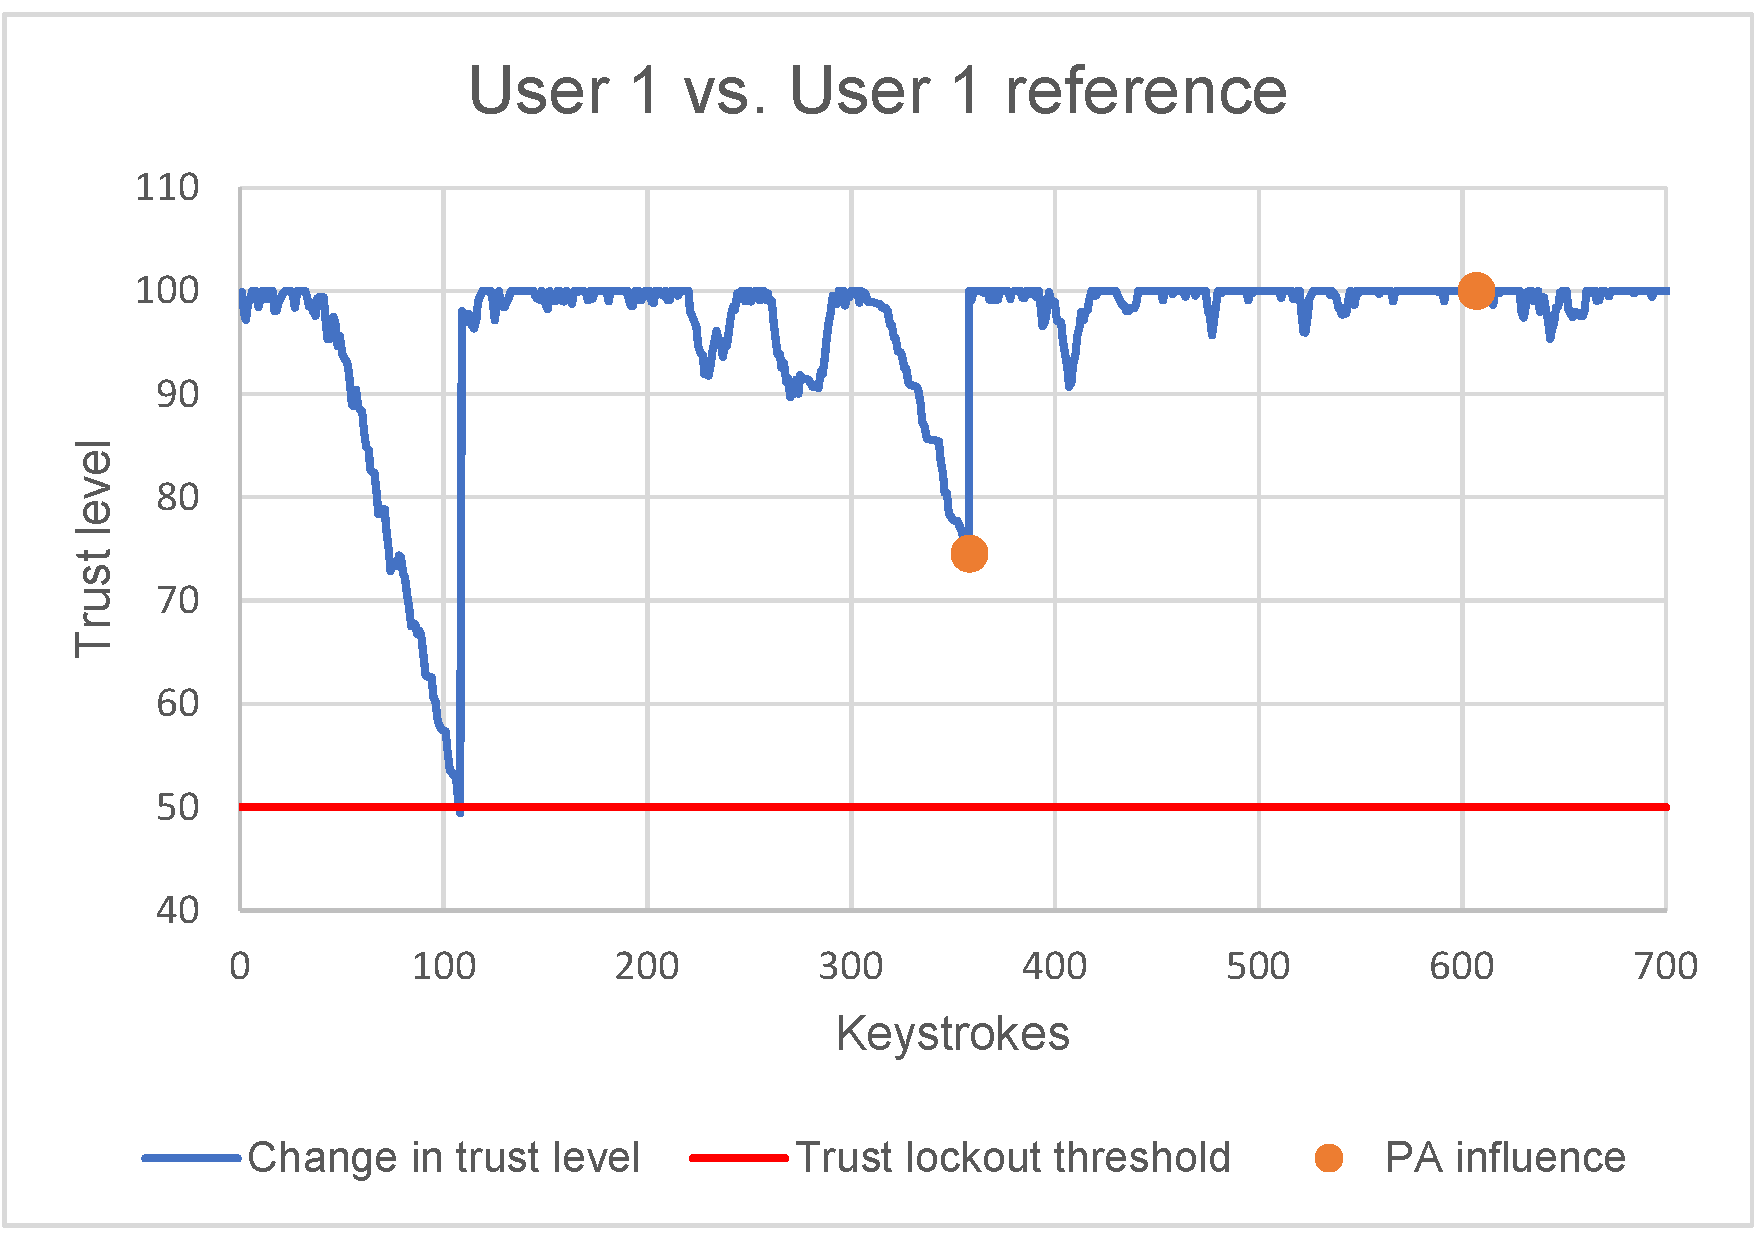
\includegraphics[width=0.8\textwidth]{figures/decision-lvl-genuine-250BL.pdf}
%    \caption{Decision level fusion with User 1 as genuine user. $\text{Up} = 100.1\%, \text{Down} = 60\%$. $BL = 250$.}
%    \label{fig:decision-lvl-genuine-250BL}
%\end{figure}
%
%\begin{figure}[ht]
%    \centering
%    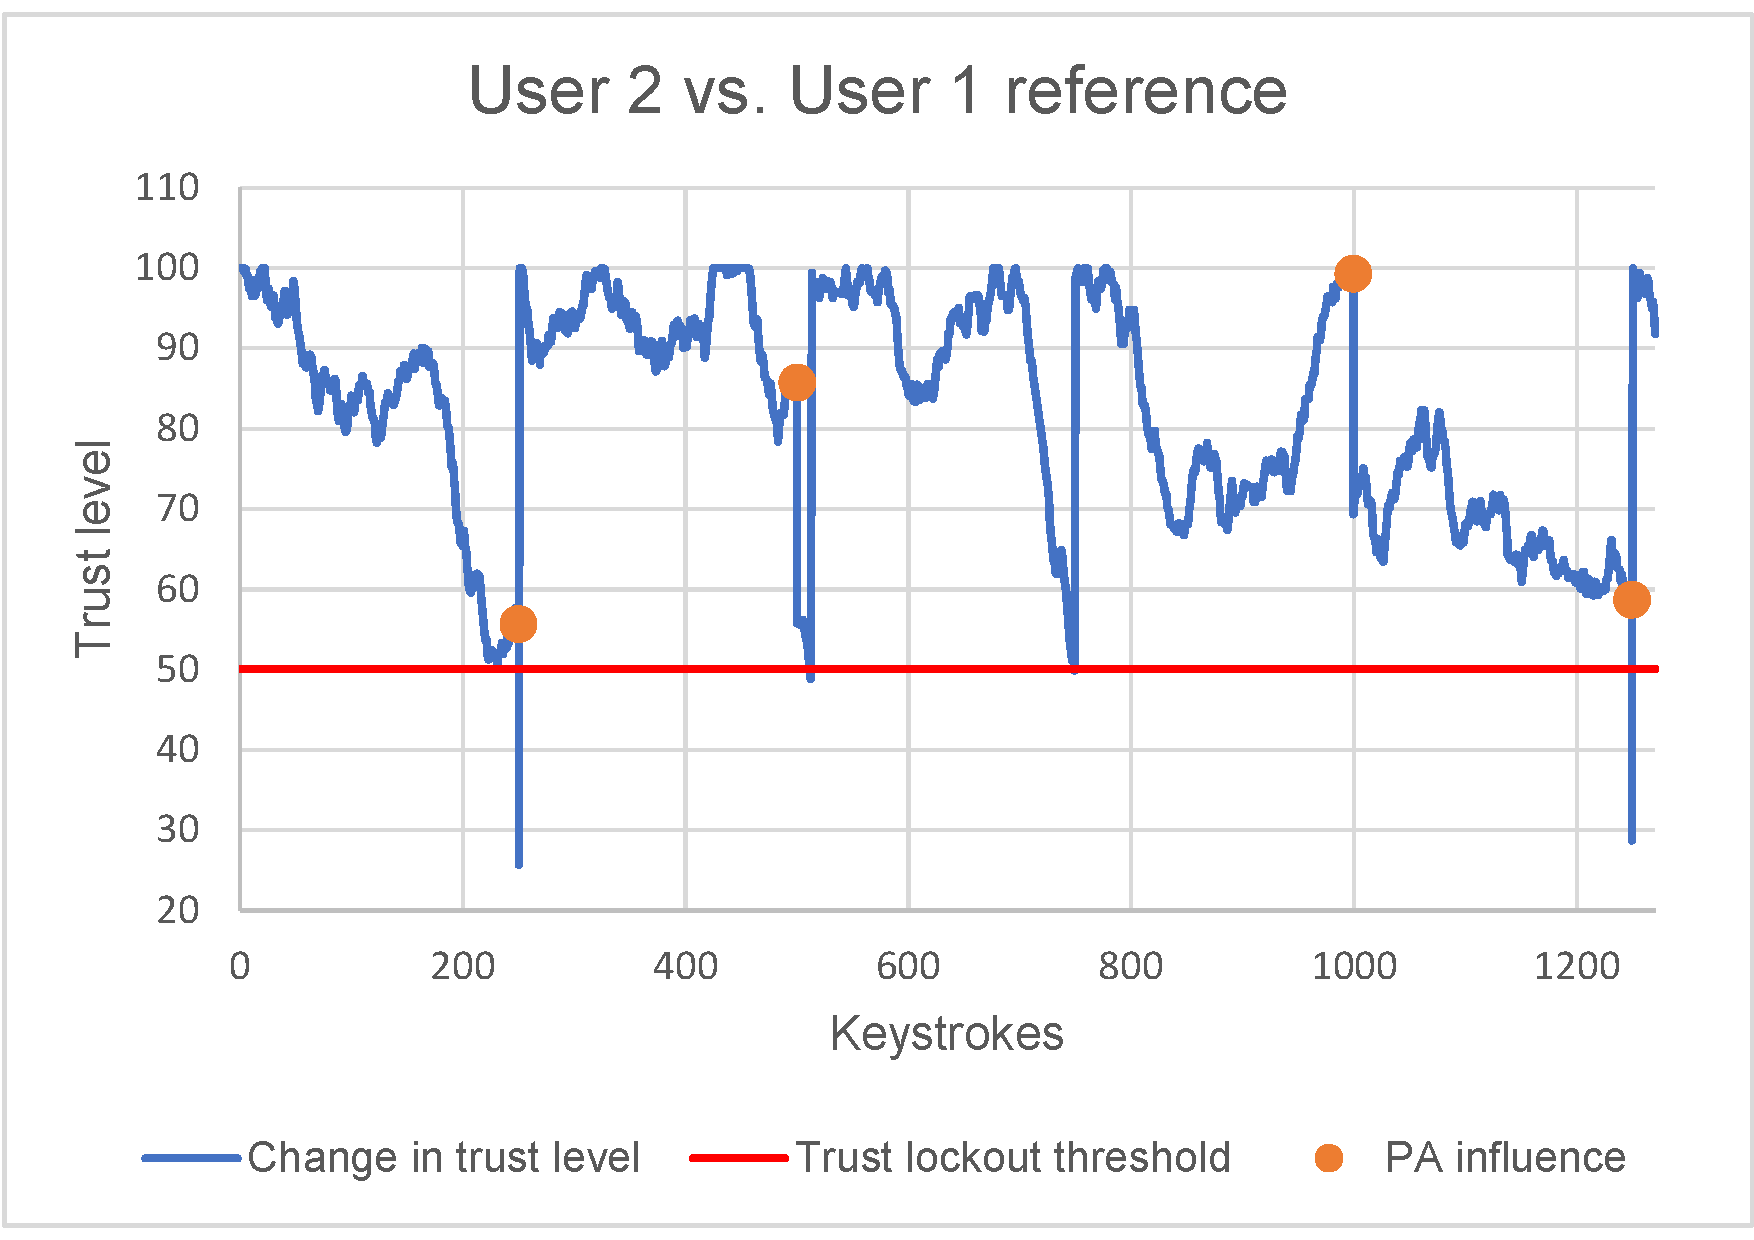
\includegraphics[width=0.8\textwidth]{figures/decision-lvl-user2-vs-user1-250BL.pdf}
%    \caption{Decision level fusion with User 2 as imposter. $\text{Up} = 100.1\%, \text{Down} = 60\%$. $BL = 250$.}
%    \label{fig:decision-lvl-user2-vs-user1-BL100}
%\end{figure}

\section{Score level fusion}
\label{sec:analysis-score-lvl}
As with the decision level fusion, the score level fusion is also based on $T_{\text{range}}$.
During testing, we gave the DTM's sigmoid function for PA influence, $\textit{Sig}_{\text{PA}}$, a height that allowed a change of trust between 0 and 50.001.
\Cref{fig:trustProgressScoreLevel} shows how the score level fusion allows the PA influence to have varying degrees of impact depending on the dissimilarity scores calculated from probe blocks.
The first of the three times the PA system kicked in, it caused a lockout by lowering the trust by 39 levels.
It kicked in again at keystroke number 333, lowering the trust by 35, meaning that block was slightly more similar to the reference than the first.
While it did not cause a direct lockout, it assisted the CA system enough for it to lock the user out at at keystroke number 535.
Lastly, we see the PA system being less decisive in its dissimilarity score, causing a drop of only 7 levels.
Because the trust level was already close to $T_{\text{lockout}}$, it still managed to nudge the trust level down just enough to cause a lockout slightly before the CA subsystem would have done so itself.

\begin{figure}[ht]
    \centering
    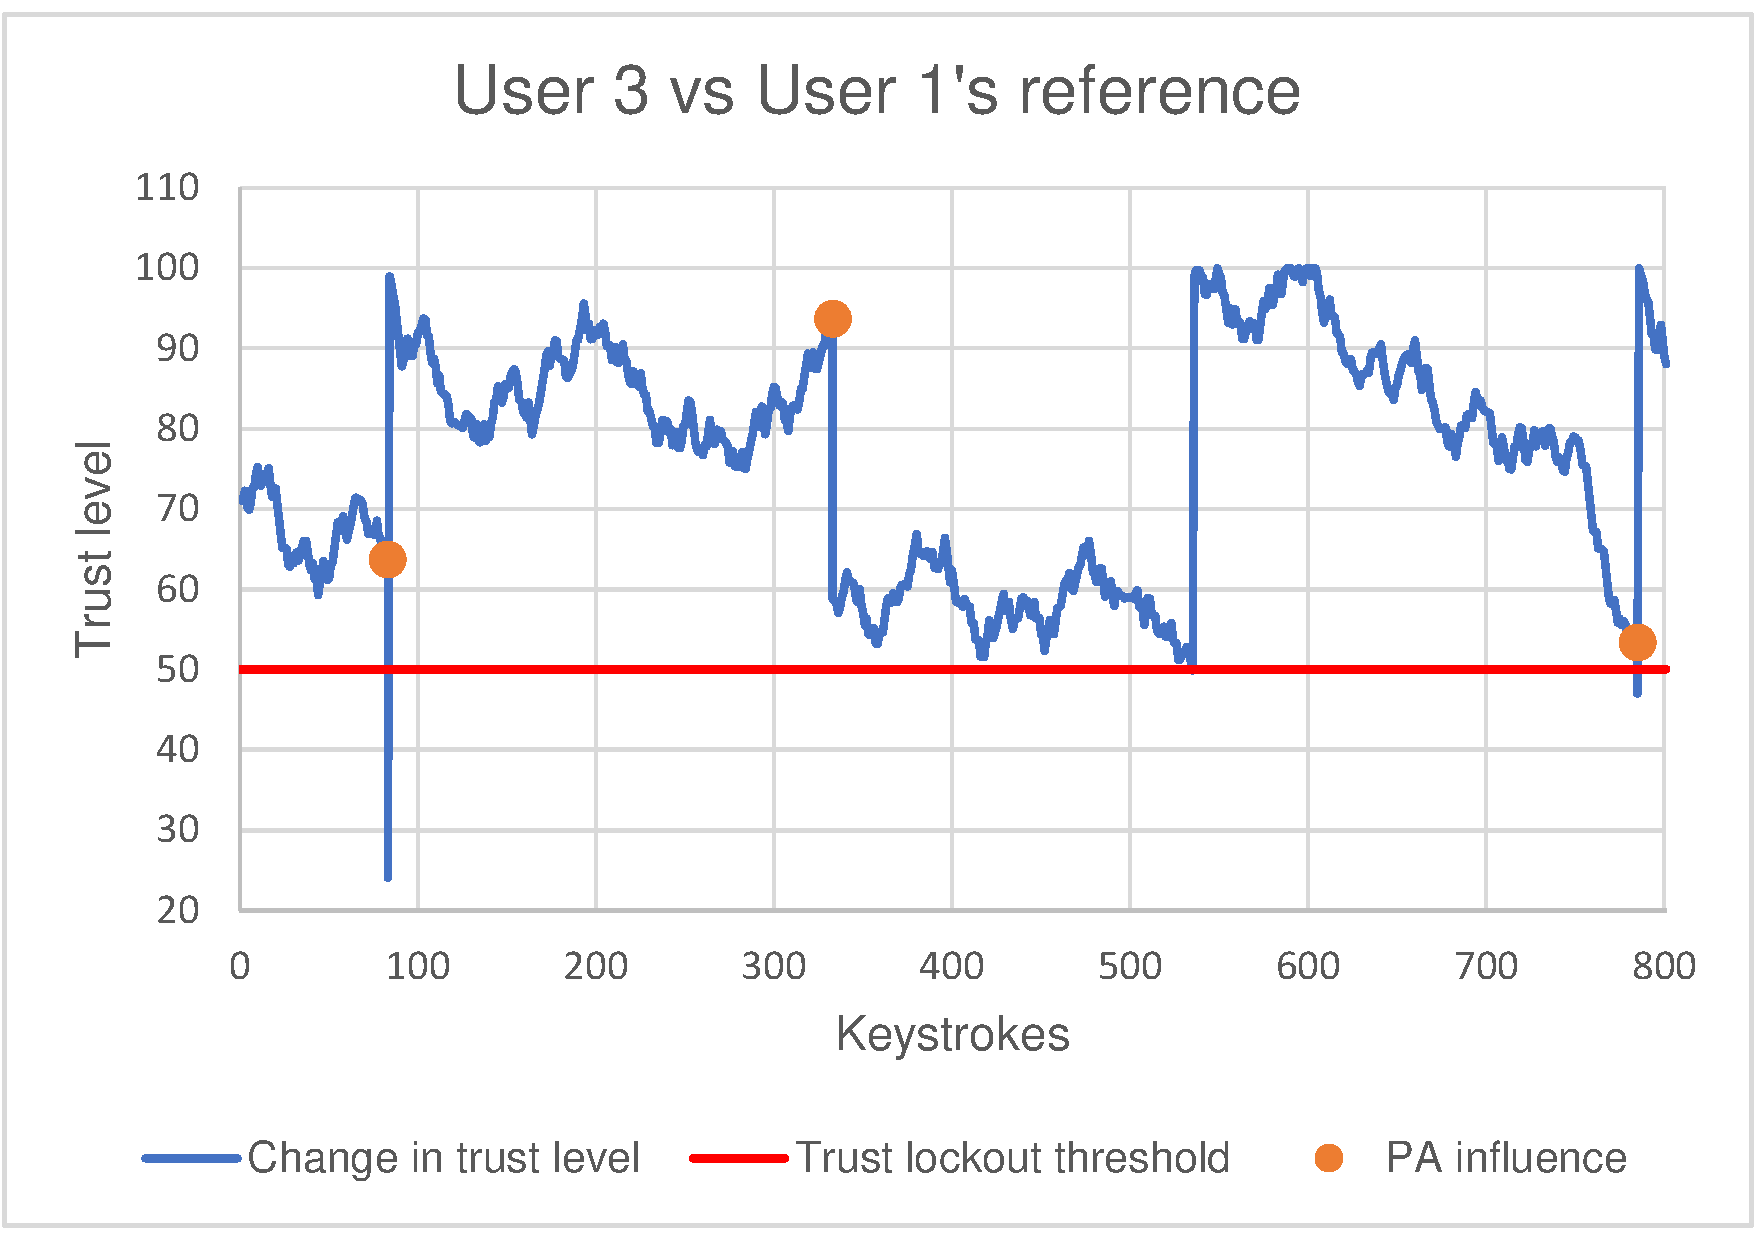
\includegraphics[width=0.8\textwidth]{figures/trustProgressScoreLevel.pdf}
    \caption{Example of score level fusion with $\text{block size} = 250$, where User 3 was tested as an imposter vs User 1's reference. DTM parameters for $\textit{Sig}_{\text{PA}}$ were as follows: $A = \text{personal} + 0.5 \text{ tolerance}$, $B = 0.1$, $C = 50.001$.}
    \label{fig:trustProgressScoreLevel}
\end{figure}

\subsection{Results}
The performance was tested by adjusting the width of $\textit{Sig}_{\text{PA}}$, as well as the PA tolerance.
The tolerance was added to the user's mean score from the validation set, similarly to the decision level fusion, however in this case it controlled the threshold for reward and penalty.
Increasing the tolerance essentially shifted $\textit{Sig}_{\text{PA}}$ towards the right.
Following are the results achieved by adjusting these parameters for different block sizes.

\subsubsection{Block size 500}
We were able to find settings improving the ANIA rating of the original CA system also with this fusion scheme. %albeit less successfully than with decision level fusion.
\Cref{tab:analysis-score-level-BL500} shows the performance using different $\textit{Sig}_{\textit{PA}}$ widths with blocks size 500.
There are more results available in the attachments, however this table is focused on results where either the ANGA or ANIA is comparable to the original CA system.
\todo{Refer directly to attachments.}
Similarly to decision level fusion, the ANGA was boosted to around 8500 when the ANIA was around the same as the CA system, being 623.
The best widths for boosting the ANGA seemed to be 0.25 and 0.3 for our specific combination and dataset, giving 8520 and 8540 ANGA while having a lower ANIA than the CA system, as well as one less undetected imposter.



\begin{table}[htbp]
\centering
\begin{tabular}{llrrr}
\hline
\textbf{Width}        & \textbf{Tolerance} & \textbf{ANGA} & \textbf{ANIA} & \textbf{\#Imp. ND} \\ \hline
\multirow{2}{*}{0.05} & 0.55               & 8097          & 539           & 13(0.6\%)          \\
                      & 0.7                & 8550          & 631           & 18(0.9\%)          \\ \hline
\multirow{2}{*}{0.1}  & 0.5                & 8094          & 560           & 13(0.6\%)          \\
                      & 0.6                & 8497          & 611           & 15(0.7\%)          \\ \hline
\multirow{2}{*}{0.25} & 0.3                & 7892          & 527           & 11(0.5\%)          \\
                      & 0.5                & 8540          & 614           & 17(0.8\%)          \\ \hline
\multirow{2}{*}{0.3}  & 0.262               & 8158          & 533          & 11(0.5\%)          \\
                      & 0.5                & 8520          & 613           & 17(0.8\%)          \\ \hline
\multirow{2}{*}{0.45} & 0.2                & 7914          & 552           & 14(0.7\%)          \\
                      & 0.5                & 8500          & 621           & 18(0.9\%)          \\ \hline
\multirow{2}{*}{0.65} & 0.3                & 8085          & 587           & 16(0.8\%)          \\
                      & 0.5                & 8432          & 629           & 18(0.9\%)          \\ \hline
\end{tabular}
\caption{Selected portions of score level fusion results with block size 500, sorted by the width of $\textit{Sig}_{\text{PA}}$.}
\label{tab:analysis-score-level-BL500}
\end{table}

Width 0.3 also seems to be the best performer for decreasing ANIA, as it was lowered to 533 while having a higher ANGA than the CA system's 8087.
The number of undetected imposters was also seven less.
In order to be able to compare the result to the decision level fusion with block size 500, we attempted to lower the tolerance in hopes of bringing the ANGA down to a rating closer to 8087.
This resulted in a 7943 ANGA and 530 ANIA, which was worse than the decision level fusion.

%This fusion scheme was also able to improve the ANIA rating of the original CA system, albeit less so than decision level fusion.


\subsubsection{Block size 250}
We observed that a larger width for $\textit{Sig}_{\text{PA}}$ was needed with block size 250.
This was clear, as widths 0.05 and 0.3 decreased the original CA system's performance apart from having one less undetected imposter, as seen in \Cref{tab:analysis-score-level-BL250}.
Both of these widths had lower ANGAs and higher ANIAs, meaning genuine users were locked out faster, while imposters had larger windows of opportunity.
At larger widths, we saw more reasonable results.
A possible cause could be the fact that smaller block sizes result in less accurate PA comparisons, as was shown in \Cref{fig:block-lengths-ROC}.
With larger sigmoid widths, comparison scores will on average cause smaller changes to the trust level. 
In other words, comparison scores are given more "wiggle room" before the influence on the trust level becomes very large, which prevents inaccurate scores to cause too much damage.
While less accurate, the smaller block sizes also cause PA comparison scores to be produced more rapidly.
Therefore, reducing the impact that each of these scores have on the trust level by increasing the width seems logical, and we believe this to be a likely explanation.

\begin{table}[htbp]
\centering
\begin{tabular}{llrrr}
\hline
\textbf{Width}        & \textbf{Tolerance} & \textbf{ANGA} & \textbf{ANIA} & \textbf{\#Imp. ND} \\ \hline
0.05                 & 0.7                & 8047          & 652           & 17(0.8\%)          \\ \hline
0.3                  & 0.7                & 7912          & 629           & 17(0.8\%)          \\ \hline
\multirow{2}{*}{0.5} & 0.35               & 7906          & 572           & 15(0.7\%)          \\
                     & 0.45               & 8745          & 623           & 21(1\%)            \\ \hline
\multirow{2}{*}{0.7} & 0.2                & 7946          & 538           & 14(0.7\%)          \\
                     & 0.5                & 8705          & 640           & 22(1.1\%)          \\ \hline
\end{tabular}
\caption{Selected excepts of score level fusion results with block size 250, sorted by the width of $\textit{Sig}_{\text{PA}}$.}
\label{tab:analysis-score-level-BL250}
\end{table}

\Cref{tab:analysis-score-level-BL250} shows that the best result for decreasing ANIA using this block size was achieved with $\text{width} = \text{0.7}$, and $\text{tolerance} = \text{0.2}$.
It gave an ANGA of 7946 and ANIA of 538, which was not as effective as the best ANIA decreasing result with block size 500.
%However, the ANIA was higher than what was achieved with block size 500, and the ANGA was also lower.
On the other hand, we saw positive results for increasing ANGA using block size 250.
With $\text{width} = \text{0.5}$, and $\text{tolerance} = \text{0.45}$, it gave an ANGA of 8745 while having the same ANIA as the original system.
This was the best ANGA improvement observed in the project's analysis phase, being an 18.4\% increase.

%Just as with decision level fusion, we see that smaller block sizes are better at improving ANGA, while larger block sizes are better at decreasing ANIA.
%Seeing this in both fusion schemes is probably no coincidence, and it raises the question of what causes such behavior.
%Looking back at \Cref{tab:PA-block-lengths}, we can see that for smaller block sizes, the tolerance levels need to be significantly higher in order to achieve high ANGA ratings.
%A possible reason is that the PA settings we have used have had lower FNMR than FMR in order to achieve reasonably high ANGA ratings.
%Therefore, when smaller block sizes are used, the PA system kicks in more often, and therefore makes



\subsubsection{Block size 100}
We performed limited testing of block size 100 with score level fusion.
However, we did test a number of different sigmoid widths, and the results in \Cref{tab:analysis-score-level-BL100} show that for ANGA values close to that of the CA system, it showed worse ANIA ratings for all widths.
We were unable to find a setting with this block size which improved the CA system's performance.
It is possible that increasing the width of $\textit{Sig}_{\text{PA}}$ is not enough to reduce the impact of inaccurate comparisons.
More research is needed to investigate this issue. 
Reducing the \text{height} of the sigmoid function to forcibly restrict the PA system from causing too large changes to the trust level could yield different results.
%It is possible that due to inaccurate comparisons, the \text{height} of the sigmoid needs to be reduced, forcibly restricting the PA system from causing too large changes to the trust level.
%More research is needed to investigate this issue.

\begin{table}[htbp]
\centering
\begin{tabular}{llrrr}
\hline
\textbf{Width} & \textbf{Tolerance} & \textbf{ANGA} & \textbf{ANIA} & \textbf{\#Imp. ND} \\ \hline
0.05           & 0.8                & 8043          & 935           & 35(1.7\%)          \\ %\hline
0.15           & 0.6                & 8010          & 771           & 30(1.4\%)          \\ %\hline
0.25           & 0.4                & 6990          & 576           & 22(1.1\%)          \\ %\hline
0.3            & 0.5                & 7927          & 715           & 29(1.4\%)          \\ %\hline
0.5            & 0.4                & 7866          & 649           & 25(1.2\%)          \\ %\hline
0.7            & 0.4                & 8015          & 652           & 23(1.1\%)          \\ %\hline
0.9            & 0.4                & 8063          & 656           & 21(1\%)            \\ %\hline
1.2            & 0.4                & 7981          & 656           & 22(1.1\%)          \\ %\hline
\end{tabular}
\caption{Selected excepts of score level fusion results with block size 100, sorted by the width of $\textit{Sig}_{\text{PA}}$.}
\label{tab:analysis-score-level-BL100}
\end{table}
%With smaller block size, more width is needed.



\todo{Get the laptop loop results from DB into schemas.}
\section{Computational impact}
\label{sec:analysis-computational-impact}
Regarding \textit{research sub-question 2}, we realize that computation speeds are highly dependent on a number of factors such as processing power, programming language, choice of classifier and number of considered features.
Still, we can mention that our CA system performs a comparison of a single keystroke in 0.2 milliseconds on average.
For our PA system, the average computing time for processing blocks of 500, 250 and 100 keystrokes was 75.2, 46 and 25.7 milliseconds, respectively.
These times were collected by finding the user with the largest reference in terms of unique mono- and digraphs, and running their validation set against their own reference.
The systems were developed in MATLAB 2017, and were run on an Intel Core i7, on a single thread at 2.4 GHz frequency.
While the speeds were reasonable, they could be further improved by for example using more a low-level programming language, not to mention as mention multi-threading.

What is most interesting to discuss is the computational impact of combining the systems.
The most important factor here is the PA subsystem's block size.
In an example where the combined system has to process 100,000 keystrokes and the block size is 100, a crude way to calculate the number of times the PA system could kick in is simply $100,000/100 = 1000$, which is the maximum.
For block size 250 and 500, it could kick in at most 400 and 200 times, respectively.
However, what must also be considered is the fact that the likelihood of the CA subsystem locking out the user before a block is filled up increases with larger block sizes.
When that happens, the PA subsystem resets and waits until enough keystrokes are recorded to fill a new block.
This further reduces computational costs when using large block sizes.

It is also important to discuss the difference between the tests we have performed and a real-time system.
During testing, we ran both the CA and PA subsystems on the same thread.
This was to avoid having the CA subsystem continuing to adjust the trust level while the PA subsystem was still processing a block probe.
If that were to happen, our results could have been less accurate.
An example could be the CA subsystem increasing an imposter's trust level before the PA subsystem had finished processing a block, and that increase of trust preventing the PA subsystem's influence from locking the user out.
Situations like these could therefore alter the performance readings.
This would not matter in a deployed real-time system as the objective would simply be to lock out imposters, and not to measure performance.
Therefore, the PA subsystem could process a block parallel to the CA system processing keystrokes with multithreading, further reducing computational impact.




\include{inc/discussion}
\chapter{Conclusion}
\label{chap:conclusion}
\todo{Future work: whenever the CA system locks out the user, let the PA system kick in earlier than usual to see if it agrees with the PA system.}
\todo{Score level fusion is less predictable than decision level fusion when it comes to adjusting parameters. More research is needed to find more predictable ways to adjust score level parameters.}
This is where you provide an overview of the thesis now that it is finished.  What are the critical things that can be learnt from the thesis for the reader.

This is additional text.

\section{Future Work}
\label{sec:future}
Maybe n-graph prediction would make smaller block sizes more viable?
Genetic algorithm for finding optimal U/D values.


\ifthenelse{\boolean{HarvardCitations}}{%
	\bibliographystyle{agsm} % used for Harvard style references. Names - Humanities & Interaction Design
}{%
	\bibliographystyle{ntnuthesis/ntnuthesis} %used for Vancover style references. Numbers - Computer Science & Physics
}

\bibliography{MastersExample}

\appendix
\chapter{PA testing data}
\label{chap:app-PA}
Following are results from testing the PA system which were not represented in the main thesis.
\section{Reference cutoff impact}
\label{sec:app-PA-reference-cutoff}
In \Cref{tab:PA-cutoff}, we only showed a excerpt of the results from testing the impact of using a reference cutoff with block size 500. Here we present the complete version of said table.
%To save space, only an excerpt of the results from testing the performance impact of using a reference cutoff was shown in \Cref{tab:PA-cutoff}. Here we present the complete version of said table.

%\subsection*{Objective}
%The Objective of this testing session was to test Hypothesis ....
%
%\subsection*{Participants}
%The participants were a convenience sample of students from NTNU. Age range $19-55$ Median age $23$ ...

%\subsection{Raw Data}
\begin{table}[htbp]
\centering
\begin{subtable}[h]{0.45\textwidth}
\begin{tabular}{lrrr}
\hline
Toler. & FNMR & FMR & \#Imp. ND  \\ \hline
0.001 & 51.98 & 4.20  & 2(0.1\%)    \\
0.003 & 51.43 & 4.24  & 2(0.1\%)    \\
0.005 & 51.15 & 4.30  & 2(0.1\%)    \\
0.008 & 50.32 & 4.36  & 2(0.1\%)    \\
0.02  & 47.51 & 4.68  & 2(0.1\%)    \\
0.04  & 43.05 & 5.29  & 3(0.1\%)    \\
0.06  & 37.75 & 5.93  & 4(0.2\%)    \\
0.08  & 33.47 & 6.66  & 4(0.2\%)    \\
0.1   & 30.25 & 7.47  & 4(0.2\%)    \\
0.12  & 26.47 & 8.30  & 5(0.2\%)    \\
0.14  & 22.97 & 9.23  & 7(0.3\%)    \\
0.16  & 19.66 & 10.31 & 8(0.4\%)    \\
0.18  & 17.77 & 11.48 & 9(0.4\%)    \\
0.2   & 15.65 & 12.71 & 11(0.5\%)   \\
0.22  & 13.40 & 14.07 & 13(0.6\%)   \\
0.24  & 11.46 & 15.53 & 14(0.7\%)   \\
0.26  & 9.44  & 17.11 & 17(0.8\%)   \\
0.28  & 8.06  & 18.77 & 20(1\%)     \\
0.3   & 6.91  & 20.52 & 22(1.1\%)   \\
0.33  & 5.48  & 23.34 & 32(1.5\%)   \\
0.35  & 4.70  & 25.37 & 37(1.8\%)   \\
0.38  & 3.64  & 28.60 & 45(2.2\%)   \\
0.4   & 2.85  & 30.80 & 54(2.6\%)   \\
0.43  & 2.07  & 34.24 & 76(3.7\%)   \\
0.45  & 1.80  & 36.67 & 87(4.2\%)   \\
0.48  & 1.34  & 40.23 & 108(5.2\%)  \\
0.5   & 1.29  & 42.61 & 121(5.8\%)  \\
%0.9   & 0.09  & 84.67 & 925(44.7\%)
 \end{tabular}
 \caption{Without reference cutoff.}
 \label{tab:app-PA-without-cutoff}
\end{subtable}
\hfill
\begin{subtable}[h]{0.45\textwidth}
\centering
\begin{tabular}{lrrr}
\hline
Toler. & FNMR  & FMR & \#Imp. ND \\ \hline
0.001 & 53.01 & 4.21  & 2(0.1\%)   \\
0.003 & 52.38 & 4.26  & 2(0.1\%)   \\
0.005 & 52.18 & 4.31  & 2(0.1\%)   \\
0.008 & 51.38 & 4.38  & 2(0.1\%)   \\
0.02  & 48.08 & 4.68  & 2(0.1\%)   \\
0.04  & 43.35 & 5.28  & 3(0.1\%)   \\
0.06  & 38.54 & 5.94  & 4(0.2\%)   \\
0.08  & 33.64 & 6.68  & 4(0.2\%)   \\
0.1   & 30.04 & 7.50  & 4(0.2\%)   \\
0.12  & 25.77 & 8.36  & 5(0.2\%)   \\
0.14  & 22.59 & 9.37  & 7(0.3\%)   \\
0.16  & 19.79 & 10.51 & 8(0.4\%)   \\
0.18  & 17.36 & 11.70 & 9(0.4\%)   \\
0.2   & 15.19 & 12.94 & 10(0.5\%)  \\
0.22  & 12.89 & 14.28 & 12(0.6\%)  \\
0.24  & 11.05 & 15.81 & 14(0.7\%)  \\
0.26  & 9.29  & 17.42 & 18(0.9\%)  \\
0.28  & 7.57  & 19.13 & 20(1\%)    \\
0.3   & 6.44  & 20.91 & 21(1\%)    \\
0.33  & 4.69  & 23.80 & 31(1.5\%)  \\
0.35  & 3.85  & 25.88 & 36(1.7\%)  \\
0.38  & 2.76  & 29.20 & 45(2.2\%)  \\
0.4   & 2.26  & 31.47 & 53(2.6\%)  \\
0.43  & 1.67  & 34.98 & 73(3.5\%)  \\
0.45  & 1.51  & 37.45 & 88(4.3\%)  \\
0.48  & 1.21  & 41.09 & 111(5.4\%) \\
0.5   & 1.13  & 43.55 & 126(6.1\%)
\end{tabular}
\caption{With reference cutoff.}
\label{tab:app-PA-with-cutoff}
\end{subtable}
\caption{Complete version of \Cref{tab:PA-cutoff}.}
\label{tab:app-PA-cutoff}
\end{table}






\chapter{Testing data from decision level fusion}
\label{chap:app-decision}
%Testing a reference to \Cref{chap:app-PA}.
%\section{Different UP values}
%\label{sec:app-decision-UP-values}
%
%\begin{table}[ht]
%\centering
%\begin{subtable}[h]{0.45\textwidth}
%\begin{tabular}{lrrr}
%\hline
%\textit{DOWN} & ANGA  & ANIA & \#Imp. ND \\ \hline
%%0     & 8944 & 706 & 25(1.2\%) \\
%%0.2   & 8602 & 630 & 20(1\%)   \\
%%0.4   & 8025 & 569 & 16(0.8\%) \\
%%0.6   & 7380 & 499 & 12(0.6\%) \\
%%0.8   & 7062 & 432 & 12(0.6\%) \\
%%1     & 5604 & 284 & 3(0.1\%)  \\
%%1.001 & 5239 & 273 & 2(0.1\%) THIS IS BL250 WITH 1.001 UP.
%0     & 8547 & 644 & 19(0.9\%) \\
%0.2   & 8545 & 605 & 18(0.9\%) \\
%0.4   & 8263 & 564 & 15(0.7\%) \\
%0.6   & 8089 & 508 & 11(0.5\%) \\
%0.8   & 7676 & 445 & 8(0.4\%)  \\
%1     & 6278 & 307 & 3(0.1\%)  \\
%1.001 & 6019 & 299 & 3(0.1\%)  
%\end{tabular}
% \caption{\text{$\textit{UP}=1.001$}}
% \label{tab:app-UD-difference-1.001}
%\end{subtable}
%\hfill
%
%\begin{subtable}[h]{0.45\textwidth}
%\begin{tabular}{lrrr}
%\hline
%\textit{DOWN} & ANGA  & ANIA & \#Imp. ND \\ \hline
%0     & 8547 & 644 & 19(0.9\%) \\
%0.2   & 8545 & 605 & 18(0.9\%) \\
%0.4   & 8263 & 564 & 15(0.7\%) \\
%0.6   & 8089 & 508 & 11(0.5\%) \\
%0.8   & 7676 & 445 & 8(0.4\%)  \\
%1     & 6278 & 307 & 3(0.1\%)  \\
%1.001 & 6019 & 299 & 3(0.1\%)
%\end{tabular}
% \caption{\text{$\textit{UP}=1$}}
% \label{tab:app-UD-difference-1}
%\end{subtable}
%
%
%\begin{subtable}[h]{0.45\textwidth}
%\begin{tabular}{lrrr}
%\hline
%\textit{DOWN} & ANGA  & ANIA & \#Imp. ND \\ \hline
%0     & 8547 & 644 & 19(0.9\%) \\
%0.2   & 8545 & 605 & 18(0.9\%) \\
%0.4   & 8263 & 564 & 15(0.7\%) \\
%0.6   & 8089 & 508 & 11(0.5\%) \\
%0.8   & 7676 & 445 & 8(0.4\%)  \\
%1     & 6278 & 307 & 3(0.1\%)  \\
%1.001 & 6019 & 299 & 3(0.1\%)  
%\end{tabular}
% \caption{\text{$\textit{UP}=0.8$}}
% \label{tab:app-UD-difference-0.8}
%\end{subtable}
%\hfill
%
%\begin{subtable}[h]{0.45\textwidth}
%\begin{tabular}{lrrr}
%\hline
%\textit{DOWN} & ANGA  & ANIA & \#Imp. ND \\ \hline
%0     & 8543 & 643 & 19(0.9\%) \\
%0.2   & 8541 & 604 & 18(0.9\%) \\
%0.4   & 8259 & 564 & 15(0.7\%) \\
%0.6   & 8086 & 508 & 11(0.5\%) \\
%0.8   & 7674 & 445 & 8(0.4\%)  \\
%1     & 6335 & 307 & 3(0.1\%)  \\
%1.001 & 6017 & 299 & 3(0.1\%) 
%
%\end{tabular}
% \caption{\text{$\textit{UP}=0.6$}}
% \label{tab:app-UD-difference-0.6}
%\end{subtable}
%
%
%\begin{subtable}[h]{0.45\textwidth}
%\centering
%\begin{tabular}{lrrr}
%\hline
%\textit{DOWN} & ANGA  & ANIA & \#Imp. ND  \\ \hline
%%0     & 8936 & 690 & 25(1.2\%) \\
%%0.2   & 8594 & 620 & 20(1\%)   \\
%%0.4   & 8017 & 557 & 16(0.8\%) \\
%%0.6   & 7352 & 493 & 12(0.6\%) \\
%%0.8   & 7068 & 426 & 12(0.6\%) \\
%%1     & 5607 & 282 & 3(0.1\%)  \\
%%1.001 & 5223 & 270 & 2(0.1\%) THIS IS BL250 WITH 0.4 UP
%0     & 8543 & 642 & 19(0.9\%) \\
%0.2   & 8541 & 603 & 18(0.9\%) \\
%0.4   & 8261 & 563 & 15(0.7\%) \\
%0.6   & 8088 & 507 & 11(0.5\%) \\
%0.8   & 7676 & 444 & 8(0.4\%)  \\
%1     & 6366 & 306 & 3(0.1\%)  \\
%1.001 & 6018 & 298 & 3(0.1\%)  
% \end{tabular}
%\caption{$\textit{UP} = 0.4$}
%\label{tab:app-UD-difference-0.4}
%\end{subtable}
%
%\hfill
%
%\begin{subtable}[h]{0.45\textwidth}
%\centering
%\begin{tabular}{lrrr}
%\hline
%\textit{DOWN} & ANGA  & ANIA & \#Imp. ND  \\ \hline
%0     & 8134 & 638 & 19(0.9\%) \\
%0.2   & 8132 & 599 & 18(0.9\%) \\
%0.4   & 7850 & 558 & 15(0.7\%) \\
%0.6   & 7676 & 503 & 11(0.5\%) \\
%0.8   & 7264 & 441 & 8(0.4\%)  \\
%1     & 5869 & 304 & 3(0.1\%)  \\
%1.001 & 5612 & 296 & 3(0.1\%)  
% \end{tabular}
%\caption{$\textit{UP} = 0.2$}
%\label{tab:app-UD-difference-0.2}
%\end{subtable}
%
%\caption{Differences in performance when adjusting \textit{DOWN} parameter for different \textit{UP} values. Block size was 500 and PA tolerance was 0.33.}
%\label{tab:app-UD-difference}
%\end{table}

\section{Other PA tolerance levels}
\label{sec:app-other-ANGAs}
Different PA tolerance levels were tested for the different block lengths when testing the decision level fusion.
Below are the resulting performance ratings when using tolerance levels other than those covered in \Cref{sec:analysis-decision-lvl-results}.

\begin{table}[ht]
\centering
\begin{subtable}[h]{0.45\textwidth}
\begin{tabular}{lrrr}
\hline
\textit{DOWN} & ANGA  & ANIA & \#Imp. ND \\ \hline
0.1   & 8550 & 648 & 20(1\%)   \\
0.2   & 8550 & 628 & 20(1\%)   \\
0.4   & 8436 & 590 & 17(0.8\%) \\
0.6   & 8325 & 535 & 13(0.6\%) \\
0.7   & 8057 & 510 & 10(0.5\%) \\
%0.75  & 8002 & 500 & 10(0.5\%) \\
0.8   & 7976 & 481 & 10(0.5\%) \\
1     & 7690 & 354 & 3(0.1\%)  \\
1.001 & 7543 & 345 & 3(0.1\%)

\end{tabular}
 \caption{$\text{PA tolerance} = 0.4$, \text{$\textit{UP}=1.001$}. PA subsystem's ANGA was 22130 and ANIA was 730.}
 \label{tab:app-BL500-tol-0.4}
\end{subtable}
\hfill
\begin{subtable}[h]{0.45\textwidth}
\centering
\begin{tabular}{lrrr}
\hline
\textit{DOWN} & ANGA  & ANIA & \#Imp. ND  \\ \hline
0.1   & 8460 & 611 & 18(0.9\%) \\
0.2   & 8458 & 591 & 18(0.9\%) \\
0.4   & 7932 & 543 & 14(0.7\%) \\
0.6   & 7432 & 474 & 8(0.4\%)  \\
0.8   & 7009 & 392 & 5(0.2\%)  \\
1     & 4211 & 265 & 2(0.1\%)  \\
1.001 & 2936 & 256 & 2(0.1\%) 

 \end{tabular}
 \caption{$\text{PA tolerance} = 0.22$, \text{$\textit{UP}=1.001$}. PA subsystem's ANGA was 3880 and ANIA was 583.}
\label{tab:app-BL500-tol-0.22}
\end{subtable}

\caption{Other PA tolerance levels with block size 500}
\label{tab:app-BL500-diffANGAs}
\end{table}



\begin{table}[ht]
\centering
\begin{subtable}[h]{0.45\textwidth}
\begin{tabular}{lrrr}
\hline
\textit{DOWN} & ANGA  & ANIA & \#Imp. ND \\ \hline
0.2   & 8812 & 655 & 22(1.1\%) \\
0.4   & 8293 & 606 & 18(0.9\%) \\
0.6   & 7544 & 555 & 15(0.7\%) \\
0.8   & 7263 & 486 & 13(0.6\%) \\
1.001 & 6560 & 348 & 4(0.2\%) 

\end{tabular}
 \caption{$\text{PA tolerance} = 0.5$, \text{$\textit{UP}=0.4$}. PA subsystem's ANGA was 12634 and ANIA was 476.}
 \label{tab:app-BL250-tol-0.5}
\end{subtable}
\hfill
\begin{subtable}[h]{0.45\textwidth}
\centering
\begin{tabular}{lrrr}
\hline
\textit{DOWN} & ANGA  & ANIA & \#Imp. ND  \\ \hline
0.1   & 8388 & 594 & 18(0.9\%) \\
0.2   & 7963 & 548 & 15(0.7\%) \\
0.4   & 6859 & 459 & 8(0.4\%)  \\
0.6   & 6385 & 369 & 5(0.2\%)  \\
0.8   & 4933 & 291 & 4(0.2\%)  \\
1     & 1152 & 173 & 1(0\%)    \\
1.001 & 872  & 167 & 1(0\%) 
 \end{tabular}
 \caption{$\text{PA tolerance} = 0.14$, \text{$\textit{UP}=1.001$}. PA subsystem's ANGA was 993 and ANIA was 282.}
\label{tab:app-BL250-tol-0.14}
\end{subtable}

\caption{Other PA tolerance levels with block size 250}
\label{tab:app-BL250-diffANGAs}
\end{table}



\begin{table}[ht]
\centering
\begin{tabular}{lrrr}
\hline
\textit{DOWN} & ANGA  & ANIA & \#Imp. ND \\ \hline
0.1   & 9554 & 886 & 41(2\%)   \\
0.2   & 9128 & 782 & 33(1.6\%) \\
0.4   & 7568 & 609 & 23(1.1\%) \\
0.6   & 7174 & 447 & 13(0.6\%) \\
0.8   & 5335 & 320 & 6(0.3\%)  \\
1     & 3030 & 197 & 1(0\%)    \\
1.001 & 2151 & 189 & 0(0\%)  
\end{tabular}
\caption{PA tolerance level 0.4 with block size 100. PA subsystem's ANGA was 1539 and ANIA was 173.}
\label{tab:app-BL100-diffANGAs}
\end{table}

\chapter{Testing data from score level fusion}
\label{chap:app-score}
Here, we show all results from testing the score level fusion. 
The results are categorized by block sizes, and the following tables are extensions of the tables displayed in \Cref{sec:analysis-score-lvl-results}.

\section{Block size 500}
\label{sec:app-score-BL500}

\begin{center}
\begin{longtable}{llrrr}
\caption[Complete version of \Cref{tab:analysis-score-level-BL500}.]{Complete version of \Cref{tab:analysis-score-level-BL500}.} \label{tab:app-score-BL500} \\

\hline \multicolumn{1}{l}{\textbf{Width}} & \multicolumn{1}{l}{\textbf{Toler.}} & \multicolumn{1}{r}{\textbf{ANGA}} & \multicolumn{1}{r}{\textbf{ANIA}} & \multicolumn{1}{r}{\textbf{\#Imp. ND}} \\ \hline 
%\hline
%\textbf{Width} & \textbf{Toler.} & \textbf{ANGA} & \textbf{ANIA} & \textbf{\#Imp. ND}
%\hline
\endfirsthead

\multicolumn{5}{c}%
{{\bfseries \tablename\ \thetable{} -- continued from previous page}} \\
%\hline \multicolumn{1}{|c|}{\textbf{Time (s)}} &
%\multicolumn{1}{c|}{\textbf{Triple chosen}} &
%\multicolumn{1}{c|}{\textbf{Other feasible triples}} \\ \hline 
\hline \multicolumn{1}{l}{\textbf{Width}} & \multicolumn{1}{l}{\textbf{Toler.}} & \multicolumn{1}{r}{\textbf{ANGA}} & \multicolumn{1}{r}{\textbf{ANIA}} & \multicolumn{1}{r}{\textbf{\#Imp. ND}} \\ \hline
\endhead

\hline \multicolumn{5}{|r|}{{Continued on next page}} \\ \hline
\endfoot

\hline \hline
\endlastfoot

%\multirow{6}{*}{0.05} 
0.05 & 0.4   & 7936 & 449 & 9(0.4\%)  \\
                      & 0.5   & 8026 & 510 & 12(0.6\%) \\
                      & 0.55  & 8097 & 539 & 13(0.6\%) \\
                      & 0.6   & 8212 & 572 & 13(0.6\%) \\
                      & 0.7   & 8550 & 631 & 18(0.9\%) \\
                      & 0.8   & 8550 & 670 & 22(1.1\%) \\ \hline
%\multirow{9}{*}{0.1}  
 0.1                       & 0     & 5424 & 285 & 3(0.1\%)  \\
                      & 0.1   & 6186 & 333 & 4(0.2\%)  \\
                      & 0.2   & 7446 & 394 & 7(0.3\%)  \\
                      & 0.3   & 7746 & 440 & 9(0.4\%)  \\
                      & 0.4   & 7996 & 494 & 11(0.5\%) \\
                      & 0.5   & 8094 & 560 & 13(0.6\%) \\
                      & 0.6   & 8497 & 611 & 15(0.7\%) \\
                      & 0.7   & 8550 & 660 & 22(1.1\%) \\
                      & 0.8   & 8550 & 678 & 22(1.1\%) \\ \hline
%\multirow{9}{*}{0.15} 
                       0.15 & 0     & 6188 & 340 & 4(0.2\%)  \\
                      & 0.1   & 6805 & 385 & 5(0.2\%)  \\
                      & 0.2   & 7558 & 434 & 8(0.4\%)  \\
                      & 0.3   & 7949 & 478 & 10(0.5\%) \\
                      & 0.4   & 8014 & 527 & 11(0.5\%) \\
                      & 0.5   & 8087 & 590 & 15(0.7\%) \\
                      & 0.6   & 8548 & 637 & 20(1\%)   \\
                      & 0.7   & 8550 & 667 & 22(1.1\%) \\
                      & 0.8   & 8550 & 683 & 22(1.1\%) \\ \hline
%\multirow{9}{*}{0.2}
                        0.2 & 0     & 6376 & 380 & 5(0.2\%)  \\
                      & 0.1   & 6963 & 421 & 6(0.3\%)  \\
                      & 0.2   & 7665 & 468 & 10(0.5\%) \\
                      & 0.3   & 7919 & 509 & 11(0.5\%) \\
                      & 0.4   & 8067 & 550 & 11(0.5\%) \\
                      & 0.5   & 8487 & 614 & 19(0.9\%) \\
                      & 0.6   & 8544 & 645 & 20(1\%)   \\
                      & 0.7   & 8550 & 670 & 22(1.1\%) \\
                      & 0.8   & 8550 & 684 & 23(1.1\%) \\ \hline
%\multirow{9}{*}{0.25} 
                    0.25 & 0     & 6667 & 419 & 6(0.3\%)  \\
                      & 0.1   & 7258 & 449 & 8(0.4\%)  \\
                      & 0.2   & 7355 & 496 & 11(0.5\%) \\
                      & 0.3   & 7892 & 527 & 11(0.5\%) \\
                      & 0.4   & 8352 & 575 & 14(0.7\%) \\
                      & 0.5   & 8540 & 614 & 17(0.8\%) \\
                      & 0.6   & 8544 & 652 & 20(1\%)   \\
                      & 0.7   & 8544 & 673 & 22(1.1\%) \\
                      & 0.8   & 8554 & 682 & 23(1.1\%) \\ \hline
%\multirow{12}{*}{0.3}
                    0.3 & 0     & 6763 & 443 & 8(0.4\%)  \\
                      & 0.1   & 7178 & 472 & 9(0.4\%)  \\
                      & 0.2   & 7410 & 512 & 11(0.5\%) \\
                      & 0.25  & 7943 & 529 & 11(0.5\%) \\
                      & 0.265 & 8158 & 534 & 11(0.5\%) \\
                      & 0.28  & 8160 & 540 & 11(0.5\%) \\
                      & 0.3   & 8160 & 546 & 12(0.6\%) \\
                      & 0.4   & 8447 & 583 & 16(0.8\%) \\
                      & 0.5   & 8520 & 613 & 17(0.8\%) \\
                      & 0.6   & 8544 & 655 & 21(1\%)   \\
                      & 0.7   & 8544 & 670 & 21(1\%)   \\
                      & 0.8   & 8548 & 682 & 23(1.1\%) \\ \hline
%\multirow{9}{*}{0.35}
                    0.35 & 0     & 7005 & 461 & 8(0.4\%)  \\
                      & 0.1   & 7279 & 498 & 10(0.5\%) \\
                      & 0.2   & 7860 & 528 & 11(0.5\%) \\
                      & 0.3   & 8214 & 558 & 14(0.7\%) \\
                      & 0.4   & 8497 & 588 & 16(0.8\%) \\
                      & 0.5   & 8520 & 618 & 17(0.8\%) \\
                      & 0.6   & 8540 & 656 & 21(1\%)   \\
                      & 0.7   & 8544 & 672 & 22(1.1\%) \\
                      & 0.8   & 8548 & 681 & 23(1.1\%) \\ \hline
%\multirow{9}{*}{0.4}  
                    0.4 & 0     & 7268 & 482 & 9(0.4\%)  \\
                      & 0.1   & 7582 & 512 & 10(0.5\%) \\
                      & 0.2   & 7882 & 544 & 13(0.6\%) \\
                      & 0.3   & 8214 & 566 & 15(0.7\%) \\
                      & 0.4   & 8429 & 596 & 16(0.8\%) \\
                      & 0.5   & 8500 & 620 & 17(0.8\%) \\
                      & 0.6   & 8520 & 655 & 21(1\%)   \\
                      & 0.7   & 8547 & 673 & 22(1.1\%) \\
                      & 0.8   & 8547 & 681 & 23(1.1\%) \\ \hline
%\multirow{9}{*}{0.45}
                        0.45 & 0     & 7273 & 500 & 10(0.5\%) \\
                      & 0.1   & 7584 & 522 & 11(0.5\%) \\
                      & 0.2   & 7914 & 552 & 14(0.7\%) \\
                      & 0.3   & 8382 & 575 & 16(0.8\%) \\
                      & 0.4   & 8428 & 597 & 16(0.8\%) \\
                      & 0.5   & 8500 & 621 & 18(0.9\%) \\
                      & 0.6   & 8520 & 646 & 19(0.9\%) \\
                      & 0.7   & 8547 & 672 & 22(1.1\%) \\
                      & 0.8   & 8547 & 680 & 23(1.1\%) \\ \hline
%\multirow{5}{*}{0.65}
                    0.65 & 0.3   & 8085 & 587 & 16(0.8\%) \\
                      & 0.4   & 8399 & 609 & 17(0.8\%) \\
                      & 0.5   & 8432 & 629 & 18(0.9\%) \\
                      & 0.7   & 8504 & 654 & 20(1\%)   \\
                      & 0.9   & 8547 & 683 & 23(1.1\%)
\end{longtable}
\end{center}

%\include{inc/timetable}

\end{document}
